% Clicker Question Bank for Numerical Analysis
% 
% [Open Access License here]
%
% If you have any comments, criticisms, or additions to this question
% bank, then please contact the authors.
%
% Authors: John M. Stockie (jstockie@sfu.ca) - JMS
%          M. Alamgir Hossain (mahossai@sfu.ca) - MAH
%          Department of Mathematics
%          Simon Fraser University
%          Burnaby, British Columbia, Canada
% 
% Website: All LaTeX source, images and Matlab code used to produce them
%          can be found at this URL.
%
% Current revision: 1.0
% Revision date:    April 7, 2020
%
% TO DO LIST:
% * more T/F and shorter questions in all sections
% * add a few more questions on the Secant Method (2c)
% * nothing yet for Fractals and Nonlinear Systems (2e)
% * nothing yet for Eigenvalue Problems (3e)
% * a few more interpolation/fitting applications (4e)
% * nothing yet for Stability and Implicit Methods (6e)

\documentclass[10pt]{article}

%%%%%%%%%%%%%%%%%%%%%%%%%%%%%%%%%%%%%%%%%%%%%%%%%%%%%%%%%%%%%%%%%%%%%%
\usepackage{amsmath,amssymb}
\usepackage{graphicx,color}
\usepackage{calc,ifthen}
\usepackage{xspace}
% \usepackage{enumitem}  % this breaks beamer
\usepackage{alphalph}
%\usepackage{url}
\usepackage{arydshln}
 
\usepackage{tikz}  % for \circnum
\usetikzlibrary{calc}
\usepackage{hyperref}
%\usepackage[hyperpageref]{backref}

% clickerdefs.tex: LaTeX definitions that are common to all 
% formats used to display clicker questions (question bank, 
% beamer, etc.)

\newcommand{\courseID}{MACM~316\xspace} % at SFU
\newcommand{\coursename}{Numerical Analysis~I\xspace}
\newcommand{\clickerVersion}{1.0}
\newcommand{\clickerDate}{May 14, 2020}

\newcommand{\CClicense}{%
  \begin{center}
    \includegraphics[height=1cm]{cc-by-nc-sa.png}
  \end{center}
  This teaching resource (including \LaTeX\ source, graphical images and
  \Matlab code) is made available under the Creative Commons
  \mbox{``CC~BY-NC-SA''} license.  This license allows anyone to reuse,
  revise, remix and redistribute the databank of clicker questions
  provided that it is not for commercial purposes and that appropriate
  credit is given to the original authors.  For more information, visit
  \url{http://creativecommons.org/licenses/by-nc-sa/4.0}.}

\newcommand{\mysmblank}{\underline{\phantom{aaa}}\xspace}
\newcommand{\myblank}{\underline{\phantom{aaaaaa}}\xspace}
\newcommand{\mybigblank}{\underline{\phantom{aaaaaaaaaaaa}}\xspace}
\newcommand{\fillblank}{\emph{Fill in the blank:}~}
\newcommand{\fillblanks}{\emph{Fill in the blanks:}~}
\newcommand{\myuline}[1]{\underline{\smash{#1}}}
\newcommand{\theblank}{{\tt [blank]}}
%\newcommand{\circnum}[1]{\raisebox{0.5pt}{\mbox{\textcircled{\raisebox{-0.9pt}{\mbox{\sffamily #1}}}}}}
%\newcommand{\circnum}[1]{\textcircled{{#1}}} % simpler version (fails)
\newcommand*\circnum[1]{\tikz[baseline=(char.base)]{
        \node[shape=circle,draw,minimum size=4mm, inner sep=0pt] (char)
        {\rule[-3pt]{0pt}{\dimexpr2ex+2pt}#1};}}
\newcommand{\epsM}{\varepsilon_{_{\!M}}} % machine epsilon
\newcommand{\fl}{f\!\ell}                % floating point
\newcommand{\Matlab}{Matlab\xspace}
\newcommand{\ds}[1]{{\displaystyle #1}}
\newcommand{\half}{\frac{1}{2}}
\newcommand{\cond}{\operatorname{cond}}
\newcommand{\jms}{JMS}% John M. Stockie
\newcommand{\mah}{MAH}% M. Alamgir Hossain

\newcommand{\fixthis}[1]{\textcolor{red}{\fbox{~FIX: #1~}}}
\newcommand{\leavethisout}[1]{}

\newcounter{ABCcounter}  % List with (A), (B), (C), ...
\newenvironment{ABClist}{%
  \begin{list}{(\Alph{ABCcounter})}{\usecounter{ABCcounter}}}{%
  \end{list}}

\newcounter{IVcounter}  % List with I, II, III, ...
\newenvironment{IVlist}{%
  \begin{list}{\Roman{IVcounter}.}{\usecounter{IVcounter}}}{%
  \end{list}}

% For the question "source", display nothing if 
% the argument is empty.
\newcommand{\ifsource}[1]{%
  \if\relax\detokenize{#1}\relax
     % SHOW NOTHING
  \else
     \mbox{}\\[0.2cm]
     \mbox{}\hfill{\sffamily\footnotesize \{\,Source: #1\,\}}%
  \fi}

  % custom definitions for clicker questions

\usepackage{vmargin}
\setpapersize{USletter}
\setmarginsrb{20mm}{15mm}{20mm}{15mm}{0mm}{0mm}{5mm}{10mm}
\usepackage{fancyheadings}
\pagestyle{fancy}
\lhead{}\chead{}\rhead{}
\cfoot{{\small\sffamily Clicker Question Bank for Numerical Analysis
    (Version~\clickerVersion)}}
\lfoot{\raisebox{-8pt}{\includegraphics[height=0.6cm]{cc-by-nc-sa}}}
\rfoot{\small\sffamily \thepage/\pageref{last-page}}
\renewcommand{\headrulewidth}{0pt}
\renewcommand{\footrulewidth}{0.5pt}

%%%%%%%%%%%%%%%%%%%%%%%%%%%%%%%%%%%%%%%%%%%%%%%%%%%%%%%%%%%%%%%%%%%%%%
% Definitions for macros, counters, environments, etc.
\newcounter{totalQ}\setcounter{totalQ}{1}
\newcounter{totalTF}\setcounter{totalTF}{0}
\newcounter{totalMC}\setcounter{totalMC}{0}
\newcounter{Acount}\setcounter{Acount}{0}
\newcounter{Bcount}\setcounter{Bcount}{0}
\newcounter{Ccount}\setcounter{Ccount}{0}
\newcounter{Dcount}\setcounter{Dcount}{0}
\newcounter{Ecount}\setcounter{Ecount}{0}

\newcommand{\mysecnum}{0} 
\newcommand{\myhead}[2]{%\newpage
  \section*{{\sffamily\bfseries #1.~#2}}\renewcommand{\mysecnum}{#1}}
\newcommand{\mysubhead}[2]{%
  \subsection*{{\sffamily\bfseries #1.~#2}}\renewcommand{\mysecnum}{#1}}

% Macro for two-column output.  The default sizing of columns is roughly
% half-half obtained with:
%     \mytwocol{column 1 text}{column 2 text}
% To change the proportions use an optional argument as follows:
%     \mytwocol[w]{column 1 text}{column 2 text}
% where 'w' is a fraction of \textwidth for column 1 (default: w=0.45).
\newlength{\mycoltwosize} % width of column 2
\newcommand{\mytwocol}[3][0.45]{%
  % Adjust columns to account for width of \qquad being ~ 0.04\textwidth
  \setlength{\mycoltwosize}{0.90\textwidth-#1\textwidth}
  \mbox{}\begin{minipage}[t]{{#1}\textwidth}
    #2
  \end{minipage}
  \qquad % column separation
  \begin{minipage}[t]{\mycoltwosize}
    \vspace*{0pt}
    #3
  \end{minipage}}

% Modified enumerate environment for clicker question lists. 
\newenvironment{clicklist}{%
  \begin{enumerate}
    \renewcommand{\labelenumi}{{\sffamily\bfseries Q{\mysecnum}--\arabic{enumi}.}}
    \renewcommand{\labelenumi}{{\sffamily\bfseries Q{\mysecnum}--\arabic{enumi}${}^\text{\arabic{totalQ}}$.}}
    \setlength{\itemindent}{\widthof{Q}+\labelsep}
    % [label={\sffamily\bfseries Q{\mysecnum}--\arabic*.},
    % leftmargin=\widthof{[Q9a-99]}+\labelsep]
  }{%
  \end{enumerate}}

%%%%%%%%%%%%%%%%%%%%%%%%%%%%%%%%%%%%%%%%%%%%%%%%%%%%%%%%%%%%%%%%%%%%%%%
% \qitem* : Multiple choice and True/False question item formats.
%           These are pretty-printed formats that can be varied 
%           as needed and so far come in two types:
% 
% Type A: Multiple choice formats, \qitemMC{two,three,four,five}
% Type B: True/False format, \qitemTF

\newboolean{@IsSolutionPrinted} 
\setboolean{@IsSolutionPrinted}{true}  % include solutions
%\setboolean{@IsSolutionPrinted}{false} % questions only

% A. \qitemMC* -- MC question type vary depending on the number of 
%   responses (n=2,3,4,5) and each takes the following arguments: 
%   1: question statement
%   2,3,...,1+n: n choices of answer, labelled A,B,C,...
%   2+n: correct answer, given by an integer in [1,n], 1=A, 2=B, etc.
%   3+n: notes or details on solution
%   4+n: question source
\newcommand{\qitemMCtwo}[6]{\item #1
  \begin{ABClist}
  \item #2
  \item #3
  \end{ABClist}
  \ifthenelse{\boolean{@IsSolutionPrinted}}{\emph{Answer:~~(\AlphAlph{#4}).~~~~#5}}{}%  
  \ifsource{#6}
  \stepcounter{totalQ}\stepcounter{totalMC}
  \ifthenelse{#4=1}{\stepcounter{Acount}}{%
    \ifthenelse{#4=2}{\stepcounter{Ccount}}{}}
}

\newcommand{\qitemMCthree}[7]{\item #1
  \begin{ABClist}
  \item #2
  \item #3
  \item #4
  \end{ABClist}
  \ifthenelse{\boolean{@IsSolutionPrinted}}{\emph{Answer:~~(\AlphAlph{#5}).~~~~#6}}{}%  
  \ifsource{#7}
  \stepcounter{totalQ}\stepcounter{totalMC}
  \ifthenelse{#5=1}{\stepcounter{Acount}}{%
    \ifthenelse{#5=2}{\stepcounter{Bcount}}{%
      \ifthenelse{#5=3}{\stepcounter{Ccount}}{}}}
}

\newcommand{\qitemMCfour}[8]{\item #1 
  \begin{ABClist}
  \item #2
  \item #3
  \item #4
  \item #5
  \end{ABClist}
  \ifthenelse{\boolean{@IsSolutionPrinted}}{\emph{Answer:~~(\AlphAlph{#6}).~~~~#7}}{}%
  \ifsource{#8}
  \stepcounter{totalQ}\stepcounter{totalMC}
  \ifthenelse{#6=1}{\stepcounter{Acount}}{%
    \ifthenelse{#6=2}{\stepcounter{Bcount}}{%
      \ifthenelse{#6=3}{\stepcounter{Ccount}}{%
        \ifthenelse{#6=4}{\stepcounter{Dcount}}{}}}}
}

\newcommand{\qitemMCfourtwoc}[8]{\item #1\\
  \begin{minipage}[t]{0.5\textwidth}
    \begin{ABClist}
    \item #2
    \item #3
    \end{ABClist}
  \end{minipage}
  \begin{minipage}[t]{0.5\textwidth}
    \begin{ABClist}
      \setcounter{ABCcounter}{2}
    \item #4
    \item #5
    \end{ABClist}
  \end{minipage}
  
  \ifthenelse{\boolean{@IsSolutionPrinted}}{\emph{Answer:~~(\AlphAlph{#6}).~~~~#7}}{}%
  \ifsource{#8}
  \stepcounter{totalQ}\stepcounter{totalMC}
  \ifthenelse{#6=1}{\stepcounter{Acount}}{%
    \ifthenelse{#6=2}{\stepcounter{Bcount}}{%
      \ifthenelse{#6=3}{\stepcounter{Ccount}}{%
        \ifthenelse{#6=4}{\stepcounter{Dcount}}{}}}}
}

\newcommand{\qitemMCfive}[9]{\item #1 
  \begin{ABClist}
  \item #2
  \item #3
  \item #4
  \item #5
  \item #6
  \end{ABClist}
  \ifthenelse{\boolean{@IsSolutionPrinted}}{\emph{Answer:~~(\AlphAlph{#7}).~~~~#8}}{}%
  \ifsource{#9}
  \stepcounter{totalQ}\stepcounter{totalMC}
  \ifthenelse{#7=1}{\stepcounter{Acount}}{%
    \ifthenelse{#7=2}{\stepcounter{Bcount}}{%
      \ifthenelse{#7=3}{\stepcounter{Ccount}}{%
        \ifthenelse{#7=4}{\stepcounter{Dcount}}{%
          \ifthenelse{#7=5}{\stepcounter{Ecount}}{}}}}}
}
  
% B. \qitemTF -- T/F question type takes the following arguments: 
%   1: question statement
%   2: correct answer (either TRUE or FALSE)
%   3: notes on the solution
%   4: question source
\newcommand{\qitemTF}[4]{\item \emph{True or False:} #1\\[0.3cm]
  \ifthenelse{\boolean{@IsSolutionPrinted}}{\emph{Answer:~~{#2}.~~~~#3}}{}%
  \ifsource{#4}
  \stepcounter{totalQ}\stepcounter{totalTF}
}

%%%%%%%%%%%%%%%%%%%%%%%%%%%%%%%%%%%%%%%%%%%%%%%%%%%%%%%%%%%%%%%%%%%%%% 
%%%%%%%%%%%%%%%%%%%%%%%%%%%%%%%%%%%%%%%%%%%%%%%%%%%%%%%%%%%%%%%%%%%%%% 
\begin{document}

% \everymath{\displaystyle}   % this avoids having to use \ds{}

\noindent
{\sffamily
SIMON FRASER UNIVERSITY   \hfill {M.\ Alamgir Hossain}\\
{FACULTY OF SCIENCE}      \hfill {John M. Stockie}\\
DEPARTMENT OF MATHEMATICS \hfill \\
}
\noindent
\rule{\textwidth}{0.5pt}

\begin{center}
  {\bfseries\sffamily\Large Clicker Question Bank for Numerical Analysis
    % (\courseID)
    \\
    (Version~\clickerVersion\ --\ \clickerDate)}
\end{center}
\CClicense

\noindent
\rule{\textwidth}{0.5pt}

%%%%%%%%%%%%%%%%%%%%%%%%%%%%%%%%%%%%%%%%%%%%%%%%%%%%%%%%%%%%%%%%%%%%%%%%%%%%% 
\myhead{1}{Introduction}

\begin{clicklist}
  
  \qitemMCfive{Select the best definition for ``numerical analysis'':}%
  {the study of round-off errors}% Trefethen #1
  {the study of algorithms for computing approximate solutions to
    problems from continuous
    mathematics}% Trefethen, modified by Stockie
  {the study of quantitative approximations to the solutions of
    mathematical problems including consideration of and bounds for the
    errors involved}% Merriam-Webster
  {the branch of mathematics that deals with the development and use of
    numerical methods for solving problems}% Lexico / Oxford
  {the branch of mathematics dealing with methods for obtaining
    approximate numerical solutions of mathematical
    problems}% Dictionary.com
  {2}{All 5 definitions are valid in some sense since they reflect some
    aspect of the field (most are pulled off the internet).  But my
    favourite definition is (B) because it contains three very important
    keywords underlined below:  
    \begin{center}
      the study of \myuline{algorithms} for computing
      \myuline{approximate} solutions to problems from
      \myuline{continuous} mathematics\\
      {\footnotesize [ algorithms $\Longleftrightarrow$ computing,
        \qquad
        approximate $\Longleftrightarrow$ floating point arithmetic, 
        \qquad
        continuous $\Longleftrightarrow$ solutions are smooth f'ns ]}
    \end{center}%
  }{JMS}
\end{clicklist}

\mysubhead{1a}{Floating Point Arithmetic and Error}

\begin{clicklist}
  
  \qitemMCfour{How many significant digits does the floating point
    number $0.03140 \times 10^3$ have?}%
  {6}%
  {5}%
  {4}%
  {3}%
  {3}{}{} 

  
  \qitemMCfour{Suppose that a hypothetical binary computer stores floating
    point numbers in 16-bit words as shown:
    \begin{center}
      \begin{tabular}{|c|c|cc|cccccccccccc|}\hline
        {\tiny 1}  & {\tiny 2}  & {\tiny 3}  & {\tiny 4}  & 
        {\tiny 5}  & {\tiny 6}  & {\tiny 7}  & {\tiny 8}  & 
        {\tiny 9}  & {\tiny 10} & {\tiny 11} & {\tiny 12} & 
        {\tiny 13} & {\tiny 14} & {\tiny 15} & {\tiny 16} \\
        s & \multicolumn{3}{c|}{exp} & 
        \multicolumn{12}{c|}{mantissa} \\\hline
      \end{tabular}
    \end{center}
    Bit 1 is used for the sign of the number, bit 2 for the sign of the
    exponent, bits 3-4 for the magnitude of the exponent, and the
    remaining twelve bits for the magnitude of the mantissa.  What is
    machine epsilon for this computer?}%
  {$2^{-16}$}%
  {$2^{-12}$}%
  {$2^{-8}$}%
  {$2^{-4}$}%
  {2}{Assume that rounding is used and recall that $\varepsilon_{_M}$ is
    essentially the same as unit round-off error $u=\half B^{1-t}$,
    where $B=2$ is the base and $t$ is the number of significant
    digits. The number of digits stored in the mantissa is $t=12$ and so
    $\varepsilon_{_M} \approx \half 2^{1-12}=2^{-12}$.}{}
  

  \qitemMCfive{You are working with a hypothetical binary computer that
    stores integers as unsigned 4-bit words.  What is the largest
    non-negative integer that can be represented on this computer?}%
  {$64$}%
  {$63$}%
  {$31$}%
  {$15$}%
  {$7$}%
  {4}{$(1111)_2 = 1 \times 2^0 + 1 \times 2^1 + 1 \times 2^2 + 1 \times
    2^3 = 15$.}{}


  \qitemMCfour{In 1958 the Russians developed a ternary (base-3)
    computer called \emph{Setun}, after the Setun River that flows near
    Moscow State University where it was built.  In contrast with
    today's binary computers, this machine used ``trits'' (ternary bits)
    whose three possible states can be represented as $\{0, 1, 2\}$.
    Its floating-point number system was based on 27-trit numbers, with
    9 trits reserved for the exponent and 18 for the mantissa.  What was
    the value of machine epsilon $\epsilon_{_M}$ for the \emph{Setun}?}%
  {$3^{-19}$}%
  {$3^{-18}$}%
  {$3^{-9}$}%
  {$\frac{1}{3} \cdot 2^{-18}$}%
  {2}{\mbox{}\\
    \mytwocol{Apply the formula $\epsilon_{_M}=B^{-t}$ from the notes,
      where $B=3$ is the base and $t=18$ is the number digits in the
      mantissa.  You may have noticed that I didn't mention a ``sign
      trit'' for the mantissa.  In actual fact, the floating-point
      representation on \emph{Setun} was more complicated than this and
      the sign of a number came from interpreting one specific trit as
      $\{-1, 0, +1\}$ instead.}%
    {\begin{center}
        {Setun} -- Moscow State University\\
        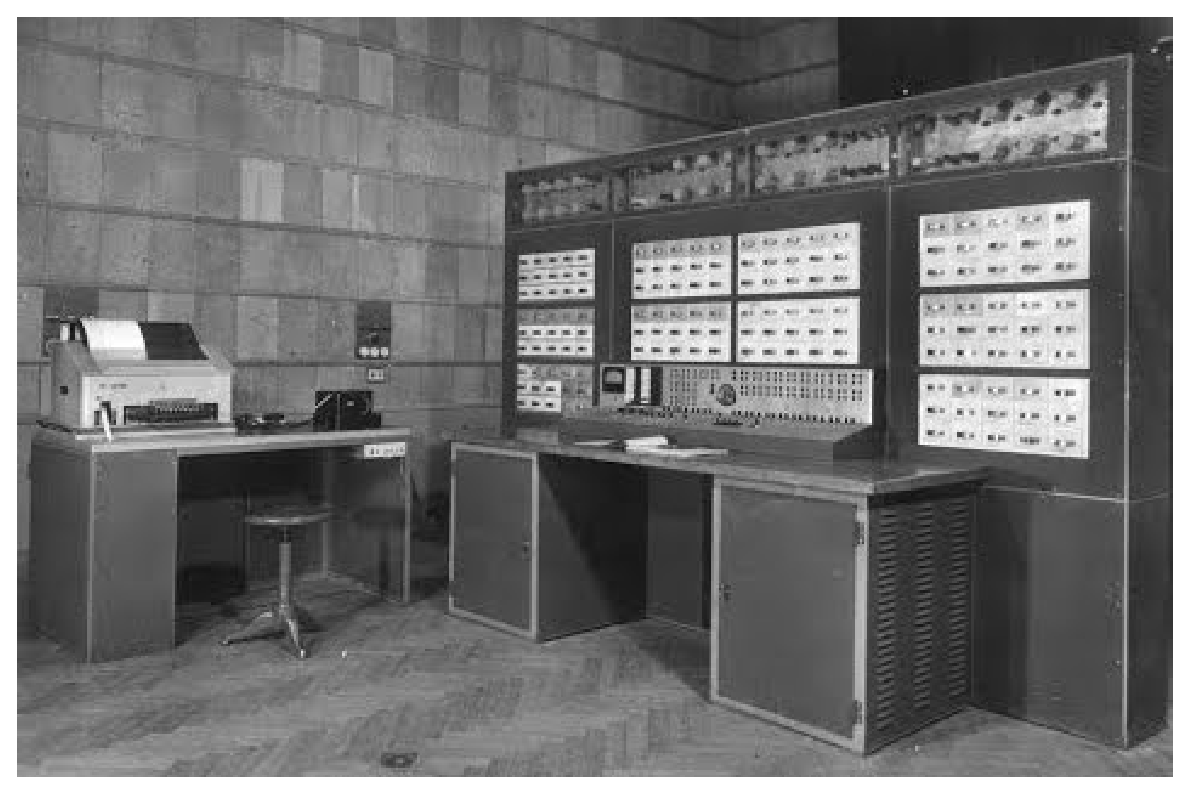
\includegraphics[width=\textwidth]{figures/setun2}
      \end{center}}}{\jms, plus info from
    \url{http://homepage.divms.uiowa.edu/~jones/ternary/numbers.shtml}}
  
  
  \qitemMCfour{In Canada, the total for any store purchase paid in cash
    is rounded to the nearest 5~cents, whereas no rounding is done if
    the payment is by credit/debit card.  Suppose that when you return
    home after purchasing your groceries with cash, you notice that your
    bill was $\$10.07$.  What is the absolute error in your actual cash
    payment?}%
  {2 cents}%
  {3 cents}%
  {4 cents}%
  {5 cents}%
  {1}{}{}
            
            
  \qitemMCfour{Let $\hat{x}$ be some approximation of
    $x$. Which of the following error definitions is correct?}%
  {absolute error = $|x - \hat{x}|$, \quad relative error =
    $\ds{\frac{|x - \hat{x}|}{|x|}}$}%
  {absolute error = $\ds{\frac{|x - \hat{x}|}{|x|}}$, \quad relative
    error = $|x - \hat{x}|$}%
  {absolute error = $\ds{\frac{|x - \hat{x}|}{|x|}, x \ne 0}$, \quad
    relative error = $|x - \hat{x}|$}%
  {absolute error = $|x - \hat{x}|$, \quad relative error =
    $\ds{\frac{|x - \hat{x}|}{|x|}, x\ne 0}$}%
  {4}{}{}
  

  \qitemMCfour{For a base-10 (decimal) floating point number $x$ having
    $t$ significant digits, the relative error satisfies
    \begin{gather*}
      R_x = \frac{|x - \fl(x)|}{|x|} \leqslant u
    \end{gather*}
    where $u$ denotes unit round-off error. Which of the following
    is true about $u$?}%
  {$u = \begin{cases}
      10^{1-t},& \text{chopping}\\
      \half 10^{1-t}, & \text{rounding}
    \end{cases}$}%
  {$u = \begin{cases}
      \half 10^{1-t},& \text{chopping}\\
      10^{1-t}, & \text{rounding}
    \end{cases}$}%
  {$u = \begin{cases}
      \half 10^{1-t},& \text{rounding}\\
      10^{1-t}, & \text{chopping}
    \end{cases}$}%
  {$u = \begin{cases}
      10^{1-t},& \text{rounding}\\
      \half 10^{1-t}, & \text{chopping}
    \end{cases}$}%
  {1}{}{}
  

  \qitemMCfour{\fillblank If $f(x)$ is a real-valued function of a real
    variable, then the \mybigblank error in the difference approximation
    for the derivative $\ds{f'(x) \approx \frac{f(x+h) - f(x)}{h}}$ goes
    to zero as $h \to 0$.}%
  {absolute}%
  {relative}%
  {cancellation}%
  {truncation}%
  {4}{Strictly, response (A) is also correct since truncation error is an
    (absolute) difference from the exact derivative.}{}
  
  
  \qitemMCfour{The two solutions of the quadratic equation $a x^2 + b x
    + c = 0$ given by
    \begin{gather*}
      x =  \frac{-b \pm \sqrt{b^2 - 4ac}}{2a}
    \end{gather*}
    are computed using floating point arithmetic.  Which of the
    statements below is TRUE?}%
  {For some values of the coefficients, this formula can generate
    cancellation errors.}%
  {If the coefficients $a$, $b$ and $c$ are very small or very large,
    then $b^2$ or $4ac$ may overflow or underflow.}%
  % {If the coefficients $a$, $b$ and $c$ are very small or very large,
  %   then $4ac$ may underflow.}%
  {The expression $\ds{x = \frac{2c}{-b \mp \sqrt{b^2 - 4ac}}}$ is an
    alternative formula for $x$ that avoids truncation error.}%
  {All of the above.}%
  {4}{}{}
  

  \qitemMCfour{In floating-point arithmetic, which of the following
    operations on two positive floating-point numbers can produce an
    overflow?}%
  {addition}%
  {subtraction}%
  {multiplication}%
  {division}%
  {1}{But (C) and (D) are also valid responses.  Let $x$ be the largest
    number that can be represented.  Then the operations $x + 1.0$, $x *
    2.0$ and $x \div 0.3$ all generate an overflow.}{Heath~\cite{heath-2018},
    Review Question 1.29, p.~40}


  \qitemMCfour{In floating-point arithmetic, which of the following
    operations on two positive floating-point numbers can produce an
    underflow?}%
  {addition}%
  {subtraction}%
  {multiplication}%
  {division}%
  {3}{But (D) is also a valid response.  Let $x$ be the smallest
    positive number that can be represented.  Then the operations $x *
    0.5$ and $x \div 2.3$ both generate an
    underflow.}{Heath~\cite{heath-2018}, Review Question 1.30, p.~40}
  

  \qitemMCfour{Let $\{x_k\}$ be a decreasing sequence of positive
    numbers with $x_{k+1}<x_k$ for $k=1,2,\dots$.  In what order
    should the sum $\ds{\sum_{k=1}^N x_k}$ be computed 
    so as to minimize round-off error?}%
  {Order the $x_k$ from largest to smallest ($1,2,\dots, N$).}%
  {Order the $x_k$ from smallest to largest ($N,\dots, 2,1$).}%
  {Sum the terms in random order.}%
  {It doesn't matter.}%
  {2}{}{Heath~\cite{heath-2018}, adapted from Review Question 1.45,
    p.~41} 


  \qitemTF{If two real numbers can be represented exactly as
    floating-point numbers, then the result of a real arithmetic
    operation on them can also be represented exactly as a
    floating-point number.}%
  {FALSE}{As a counterexample, let $x_1=\epsM$ (machine epsilon) and
    $x_2=2$, which are exact in any other binary floating point system
    (like the IEEE standard).  Then $x_1/x_2$ has no floating point
    representation.}{Heath~\cite{heath-2018}, Review Question 1.7,
    p.~39}


  \qitemMCfour{Below are four floating point approximations, each
    accompanied by its corresponding exact value.  Which approximation
    is the most accurate?}%
  {$315700$, \quad exact value $315690$}%
  {$0.0005500$, \quad exact value $0.0005510$}%
  {$8.7362\times 10^{-5}$, \quad exact value $8.7743\times 10^{-5}$}%
  {$\epsM$ (machine epsilon), \quad exact value $0$}%
  {1}{Accuracy is measured either by counting significant digits or
    computing relative error. Answer (A) has the most significant digits
    of accuracy (4 after rounding), whereas choices (B) and (C) have 2
    and 3 significant digits. The accuracy of the answer from (D) can't
    be compared because relative error formula is undefined when the
    exact answer is zero.}{\jms}


  \qitemMCfour{You are computing using a floating-point number system
    that stores a total of $t$ decimal digits in the mantissa.  If you
    perform an arithmetic computation that has a result with
    relative error $R_x$, which of the statements below is TRUE?}%
  {The number of significant digits in the answer is $t$.}%
  {The number of significant digits cannot be predicted because of
    cancellation or round-off errors.}%
  {The number of significant digits is roughly $-\log_{10}(R_x)$.}%
  {None of the above.}%
  {4}{}{\jms}


  \qitemMCfour{The relative error in an approximate solution is 0.004\%.
    The number of significant digits in the solution that we can trust
    is:}%
  {2}%
  {3}%
  {4}%
  {5}%
  {3}{This percentage corresponds to a relative error of $4\times
    10^{-5}$.  With rounding this means that the solution is accurate to
    within only 4 significant digits.}{Holistic Numerical
    Methods~\cite{kaw-2019}, {\tt quiz\_01\_02}}


  \qitemMCfour{Let $\hat{x}$ be some approximation of an exact value
    $x$.  Which of the statements below is FALSE?}%
  {The relative error is always smaller than the absolute error.}%
  {The relative error can be smaller than the absolute error provided
    $x$ is large enough.}%
  {The relative error gives a better idea of the number of correct
    significant digits.}%
  {None of the above.}%
  {1}{Because absolute error is $E_x=|x-\hat{x}|$ and relative error is
    $R_x={|x-\hat{x}|}/|x|=E_x/|x|$, the only time $R_x<E_x$ is when
    $|x|>1$.}{\jms}


  \qitemMCfour{What is the decimal equivalent of the binary number
    $110010_2$?}%
  {100}%
  {50}%
  {48}%
  {25}%
  {2}{$110010_2 = 2^5 + 2^4 + 2^1 = 32 + 16 + 2 = 50_{10}$.}{Holistic
    Numerical Methods~\cite{kaw-2019}, {\tt quiz\_01\_04}}


  \qitemMCfour{What is the binary equivalent of the decimal number
    $25.375_{10}$?}%
  {100110.011}%
  {10011.110}%
  {11001.011}%
  {10011.0011}%
  {3}{Rewrite the decimal number as a sum of powers of 2: 
    \begin{gather*}
      25.375_{10} = 16 + 8 + 1 + \frac{1}{4} + \frac{1}{8} = 2^4 + 2^3 +
      2^0 + 2^{-2} + 2^{-3} = 11001.011_2
    \end{gather*}}{Holistic Numerical Methods~\cite{kaw-2019}, {\tt
      quiz\_01\_04}}


  \qitemMCfive{Suppose that you are working with some small quantity
    $h\ll 1$.  Which of the following expressions is NOT of $O(h^4)$ as
    $h\to 0$?}% 
  {$h^5 + 7 h^4 - 0.1 h^3$}%
  {$56 h^4$}%
  {$h^{27}$}%
  {$27h^{4.3}$}%
  {All of the above}%
  {1}{Only response (A) has a term of the form $ch^p$ with $p<4$
    that goes to zero slower than $h^4$.}{\jms} 


  \qitemMCfive{Suppose that you are working with some large quantity
    $N\gg 1$.  Which of the following expressions is NOT of $O(N^4)$ as
    $N\to \infty$?}%
  {$\ds{\frac{N^6+1}{2N^2-N+1}}$}%
  {$0.0001N^4$}%
  {$N^{3.6}$}%
  {$N^4 + e^N$}%
  {All of the above}%
  {4}{Only response (D) has a term ($e^N$) that grows faster than
    $N^4$.}{\jms}

\end{clicklist}

%%%%%%%%%%%%%%%%%%%%%%%%%%%%%%%%%%%%%%%%%%%%%%%%%%%%%%%%%%%%%%%%%%%%%%%%%%%%% 
\mysubhead{1b}{Calculus Review}

\begin{clicklist}

  \qitemMCfour{When estimating $f'(2)$ for $f(x)=x$ using the
    formula $\ds{f'(x) \approx \frac{f(x+h)-f(x)}{h}}$ and $h = 0.1$,
    the truncation error is:}%
  {0}%
  {0.1}%
  {1}%
  {2}%
  {1}{This formula can be derived from the linear Taylor
    approximation, which is exact for linear functions.}{}
                                    
                                    
  \qitemMCfour{When estimating $f'(2)$ for $f(x)=x^2$ using the formula
    $\ds{f'(x) \approx \frac{f(x+h)-f(x)}{h}}$ and $h = 0.1$, the truncation
    error is:}%
  {0}%
  {0.1}%
  {1}%
  {2}%
  {2}{}{}
                                    
                                    
  \qitemMCfour{Which of the following is NOT a Taylor series for
    $f(x)$?}%
  {$\ds{f(x+h) = f(x) + f'(x) h + \frac{f''(x)}{2!} h^2 + \frac{f'''(x)}{3!}
      h^3 + \cdot\cdot\cdot}$}%
  {$\ds{f(x) = f(x_0) + f'(x_0) (x-x_0) + \frac{f''(x_0)}{2!} (x-x_0)^2 +
      \frac{f'''(x_0)}{3!} (x-x_0)^3 + \cdot\cdot\cdot}$}%
  {$\ds{f(x) = f(0) + f'(0) x + \frac{f''(0)}{2!} x^2 + \frac{f'''(0)}{3!}
      x^3 +\cdot\cdot\cdot}$}%
  {$\ds{f(x) = f(x_0) + f'(x_0) x + \frac{f''(x_0)}{2!} x^2 +
      \frac{f'''(x_0)}{3!} x^3 + \cdot\cdot\cdot}$}%
  {4}{}{} 
  
  
  \qitemMCfour{The coefficient of $x^3$ in the Taylor series for $f(x) =
    \ln(x)$ centered about $x = 1$ is:}%
  {$\ds{\frac{1}{4}}$}%
  {$\ds{\frac{1}{3}}$}%
  {$\ds{\frac{2}{3}}$}%
  {$-\ds{\frac{2}{3}}$}%
  {2}{}{}
  

  \qitemMCfive{Using the Taylor series expansion of $f(x)=\cos(x)$ near
    $x=0$, an approximation of $f(h)$ for small $h$ is:}%
  {$\ds{\frac{\sin(h)}{h}}$}%
  {$\ds{\frac{\cos(h)-1}{h}}$}%
  {$\sin(0)$}%
  {$\cos(0)$}%
  {$1 - \half \, h^2$}%
  {4}{The first term in the Taylor series is $\cos(0)=1$.  However,
    response (E) is also correct since it comes from expanding the
    Taylor series by an additional two terms:
    \begin{gather*}
      \cos(h) \approx \cos(0) - \sin(0) h - \half \cos(0) h^2 
    \end{gather*}}{}
  

  \qitemMCfive{Using the Taylor series expansion of $f(x)=\cos(x)$ near
    $x=0$, an approximation of $f'(0)$ for small $h$ is:}%
  {$\ds{\frac{\sin(h)}{h}}$}%
  {$\ds{\frac{\cos(h)-1}{h}}$}%
  {$\sin(0)$}%
  {$\cos(0)$}%
  {$1 - \frac{h^2}{2}$}%
  {2}{Expand to get $f(0+h) \approx f(0) + h f'(0)$ and then solve for
    $f'(0)$.}{}
  

  \qitemMCfour{Let $f(x)$ be a function that is differentiable on the
    interval $[-5, 5]$. If $f(-5)=10$, $f(0)=-10$, and $f(5)=10$, then
    which of the statements below must be TRUE?
    \begin{IVlist}
    \item For some $c \in (-5, 5)$, $f(c) = 0$.
    \item For some $c \in (-5, 5)$, $f'(c) = 0$.
    \end{IVlist}}%
  {I only}%
  {II only}%
  {Both I and II}%
  {Neither I nor II}%
  {3}{II follows from the Mean Value Theorem. \\[0.3cm]
    Regarding I, the Intermediate Value Theorem (IVT) doesn't apply
    directly to the interval $(-5,5)$ since $f(-5)=f(5)$.  However, $f$
    changes sign on both intervals $[-5,0]$ and $[0,5]$.  So there are 
    at least two roots in $(-5,5)$ which means that I is also true.}{\jms}
  
  
  \qitemMCfour{Let $f(x)$ be continuous and differentiable for all $x
    \in [a,b]$ as shown in the plot below. Then there exists some real
    number $c \in (a,b)$ satisfying:
    \begin{center}
      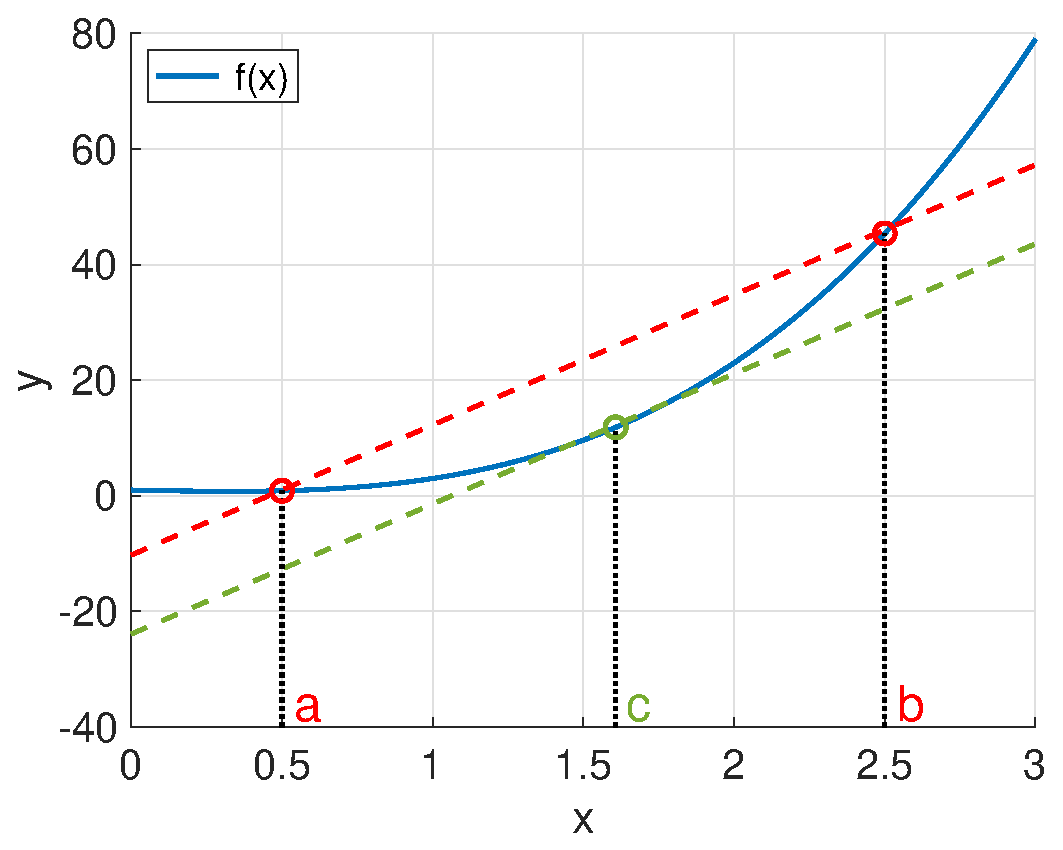
\includegraphics[width=0.45\textwidth]{figures/mvt2}
    \end{center}}%
  {$\ds{f(c) = \frac{f(b)-f(a)}{b-a}}$}%
  {$\ds{f'(c) = \frac{f(b)-b}{f(a)-a}}$}%
  {$f'(c) = 0$}%
  {$\ds{f'(c) = \frac{f(b)-f(a)}{b-a}}$}%
  {4}{This is an application of the Mean Value Theorem.}{}


  \qitemMCfour{The series $\ds{\sum_{n=0}^\infty (-4)^n
      \frac{x^{2n}}{(2n)!}}$ is the Taylor series at $x=0$ for the
    following function:}%
  {$\cos(x)$}%
  {$\cos(2x)$}%
  {$\sin(x)$}%
  {$\sin(2x)$}%
  {2}{}{Holistic Numerical Methods~\cite{kaw-2019}, {\tt quiz\_01\_07}}
  

  \qitemMCfour{Given that $f(2)=6$, $f'(2)=-\half$ and
    $f''(2)=10$, what is the most accurate Taylor polynomial
    approximation of $f(2.2)$ that you can find?}%
  {5.9}%
  {6.1}%
  {6.2}%
  {7}%
  {2}{These three point values determine the second degree Taylor
    polynomial:
    \begin{gather*}
      f(x) \approx f(2) + f'(2)(x-2) + \half f''(2)(x-2)^2 
      = 6 - \half (x-2) + \frac{10}{2}(x-2)^2 
    \end{gather*}
    and then substituting $x=2.2$ in the last expression gives
    \begin{gather*}
      f(2.2) \approx 6 - \half (0.2) + 5(0.2)^2 = 6 - 0.1 + 0.2 = 6.1
    \end{gather*}}{\jms} 
  
  
  \qitemMCfour{Which is the Taylor series for the function $\ln(x)$ at
    the point $a=1$?}%
  {$\ds{(x-1) - \half (x-1)^2 + \frac{1}{3}(x-1)^3 -
      \frac{1}{4}(x-1)^4 + \cdots}$}%
  {$\ds{(x-1) - (x-1)^2 + 2(x-1)^3 - 6(x-1)^4 + \cdots}$}%
  {$\ds{\ln(x) + \frac{1}{x}(x-1) - \frac{1}{x^2}(x-1)^2 +
      \frac{2}{x^3}(x-1)^3 - \frac{6}{x^4}(x-1)^4 + \cdots}$}%
  {$\ds{\ln(x) + \frac{1}{x}(x-1) - \frac{1}{2x^2}(x-1)^2 +
      \frac{1}{3x^3}(x-1)^3 - \frac{1}{4x^4}(x-1)^4 + \cdots}$}%
  {1}{It's easy to eliminate (C) and (D) since they are not
    polynomials.}{MathQuest~\cite{mathquest-2019}, Taylor series}
  
  
  \qitemMCfour{What function is represented by the Taylor series $\ds{1
      - \frac{x^2}{2} + \frac{x^4}{24} - \frac{x^6}{720} + \cdots}$ at
    $a=0$?}%
  {$e^x$}%
  {$\sin x$}%
  {$\cos x$}%
  {This is not a Taylor series}%
  {3}{}{MathQuest~\cite{mathquest-2019}, Taylor series}

  
  \qitemMCfour{Suppose that you determine the Taylor series for some
    function $f(x)$ centered at $a=5$.  At which point $x$ would you
    expect a finite number of terms from this series to give a better
    approximation?}%
  {$x=0$}%
  {$x=3$}%
  {$x=8$}%
  {There is no way to tell}%
  {2}{This is the closest point to $x=5$ and so the remainder term
    \myuline{suggests} that the error is smallest there.  However, the
    precise error also depends on the derivative factor $f^{(n)}(c)$ for
    some value of $c$ between $a$ and $x$, which can't be determined
    without knowing $f(x)$.  So (D) is strictly
    correct.}{MathQuest~\cite{mathquest-2019}, Taylor series}

\end{clicklist}

%%%%%%%%%%%%%%%%%%%%%%%%%%%%%%%%%%%%%%%%%%%%%%%%%%%%%%%%%%%%%%%%%%%%%%%%%%%%%%
\newpage
\myhead{2}{Nonlinear Equations}

\begin{clicklist}

  \qitemMCfour{How many zeroes does a polynomial of degree $n$ have?}%
  {$n+2$}%
  {$n+1$}%
  {$n$}%
  {$n-1$}%
  {3}{The fundamental theorem of algebra guarantees that there are
    exactly $n$ complex roots (or zeroes), some of which might be
    repeated roots.  However, if you are interested in \myuline{real}
    roots, then they could number anywhere between zero and
    $n$.}{Holistic Numerical Methods~\cite{kaw-2019}}
  

  \qitemMCfour{How many real roots does the equation $\sin(x) - x = 0$
    have?}%
  {0}%
  {1}%
  {3}%
  {Infinitely many}%
  {2}{Rewriting the equation as $\sin(x)=x$ suggests sketching the two
    functions $y = x$ and $y = \sin(x)$ on the same axes and looking for
    intersection points. Then it's easy to confirm that $x = 0$ is the
    only real root.
    \begin{flushright}
      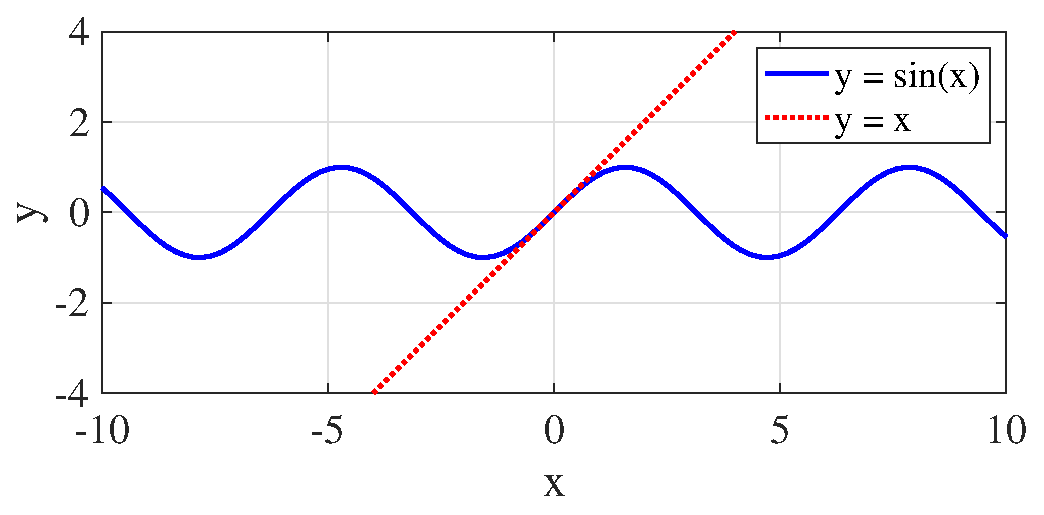
\includegraphics[width=0.45\textwidth]{figures/xsinx1}
    \end{flushright}}{\mah} 
  
  
  \qitemMCfive{How many real roots does the equation $\sin(x) - ax = 0$
    have?  ($a$ is some real constant)}%
  {0}%
  {1}%
  {3}%
  {Infinitely many}%
  {It depends on $a$}%
  {5}{By sketching the function $y=\sin(x)$ alongside various straight
    lines $y=ax$ it is easy to show that there is always at least 1 root
    ($x=0$) and that there are infinitely many roots if $a=0$.  With a
    bit more investigation, as $a$ varies there can be any odd, positive
    number of roots.  So strictly, responses (B)--(E) are all correct,
    while response (A) is not.
    \begin{flushright}
      \includegraphics[width=0.45\textwidth]{figures/xsinx}
    \end{flushright}}{\jms} 
  

  \qitemTF{When searching iteratively for a solution $x^*$ of $f(x)=0$,
    having a small value of the residual $|f(x_k)|$ guarantees that
    $x_k$ is an accurate approximation of $x^*$.}%
  {FALSE}{}{Heath~\cite{heath-2018}, Review Question 5.1, p.~245}

\end{clicklist}

%%%%%%%%%%%%%%%%%%%%%%%%%%%%%%%%%%%%%%%%%%%%%%%%%%%%%%%%%%%%%%%%%%%%%%%%%%%%%% 
\mysubhead{2a}{Bisection Method}

\begin{clicklist}

  \qitemMCfour{%
    \mytwocol{The function $f(x) = (x+1)(x-1)(x-3)$ is pictured in the
      plot.  If the bisection algorithm is applied with initial interval
      $[-4,4]$, how many roots of $f(x)$ will you be able to compute?}%
    {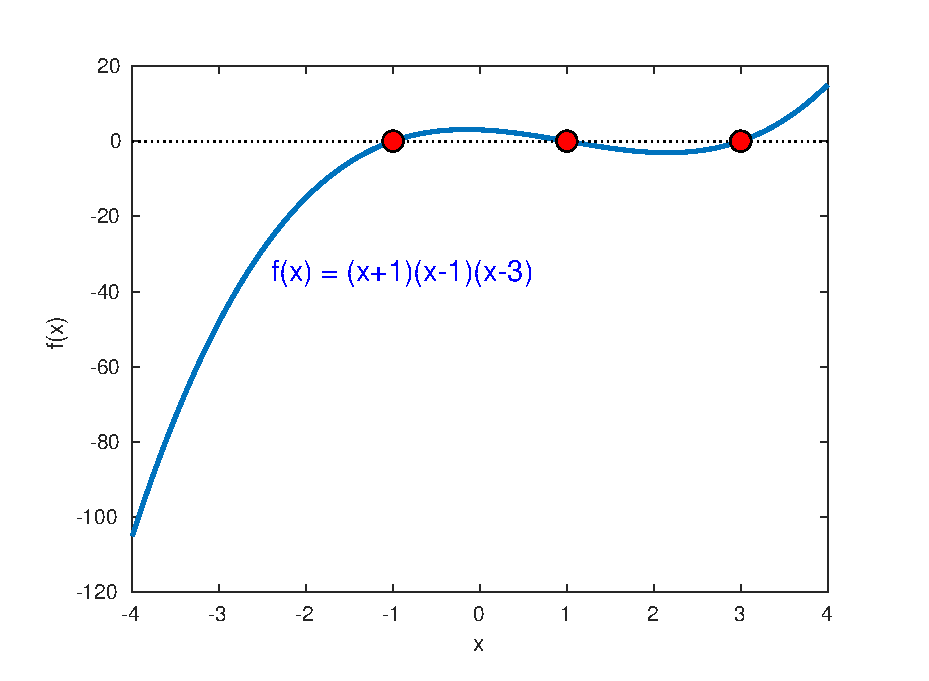
\includegraphics[width=\textwidth]{figures/bisecf}}}
    {3}%
    {2}%
  {1}%
  {none of the above}%
  {3}{All three roots $(-1$, $1$ and $3)$ lie within the interval
    $[-4,4]$, so the bisection algorithm is guaranteed to converge.
    However, the algorithm will only converge to one of those
    roots.}{\mah}

  
  \qitemTF{Let $f(x) = x^2 - 2x +1$. The bisection method can be used to
    approximate the root of the function $f(x)$ pictured.
    \begin{center}
      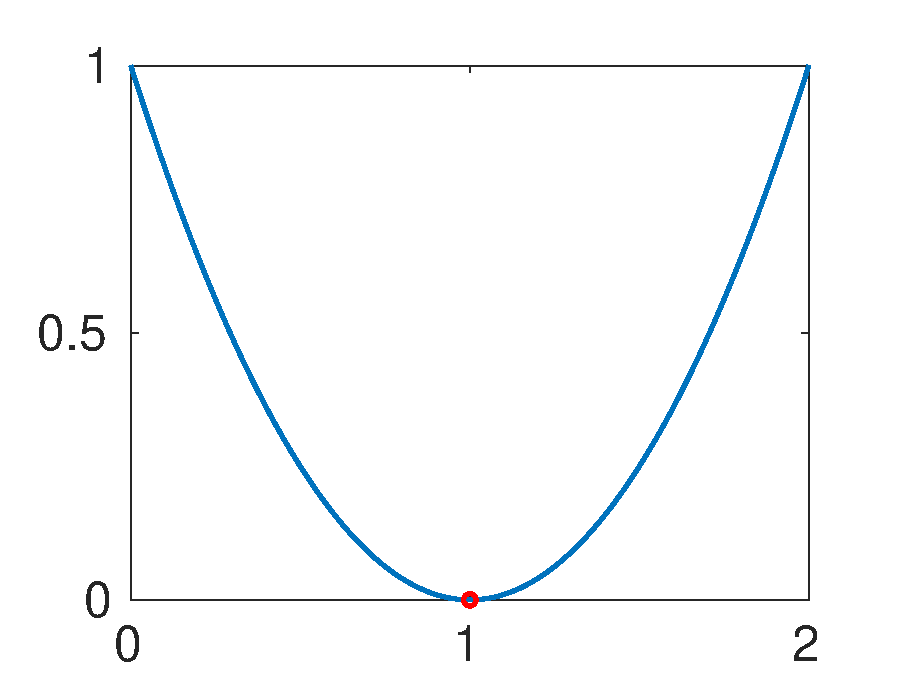
\includegraphics[width=0.45\textwidth]{figures/bisec}
    \end{center}
  \mbox{}}{FALSE}{}{\mah}

  
  \qitemMCfour{You are provided with a list of point values for the
    function $f(x) = x + 10 - e^x$: 
    \begin{center}
      \begin{tabular}{c|c|c|c|c|c}%\hline
        $x$ & 0 & 1 & 2 & 3 & 4 \\
        \hline
        $f(x)$  & 9.000  & 8.282 & 4.611 & $-$7.086 & $-$40.598 \\%\hline
      \end{tabular}
    \end{center}
    Use this data to perform two steps of the bisection method for
    solving $f(x) = 0$, assuming the initial interval $[0,4]$.  What is
    the approximation of the root?}%
  {$1$}%
  {$2$}%
  {$3$}%
  {$4$}%
  {3}{}{\courseID final exam question (Fall 2018)}
  

  \qitemMCfour{You are computing a root of $f(x)=\cos(x)-x$ on the
    interval $[0,2]$ using the bisection method.  If you require a
    result that accurate to within five significant digits, which of the
    following bounds holds for the minimum number of bisection
    iterations $k$ required?}%
  {$\ds{\frac{1}{2^{k-1}} < 10^{-5}}$}%
  {$\ds{\frac{1}{2^k} < 10^{-5}}$}%
  {$\ds{\frac{2}{2^{k+1}} < 10^{-5}}$}%
  {none of the above}%
  {1}{}{\mah}

  
  \qitemMCfour{Which of the statements below regarding the convergence
    of the bisection method is TRUE?
    \begin{IVlist}
    \item The iteration is always guaranteed to converge.
    \item The order of convergence is linear.
    \item The asymptotic rate of convergence is $\half$.
    \end{IVlist}}%
  {I and II}%
  {II and III}%
  {I and III}%
  {I, II and III}%
  {4}{All three statements are true, but only assuming that you choose
    an initial interval $[a,b]$ having $f(a)\cdot f(b) < 0$.  If that's
    not the case, then the method will not converge so none of the
    statements hold.}{\jms, \courseID lecture notes}
   

  \qitemMCfour{You are given an interval $[a,b]$ where $f(a) \cdot f(b)
    < 0$. Which of the statements below regarding the bisection method
    is TRUE?
    \begin{IVlist}
    \item There must be a root $x^*$ somewhere in the interval $(a,b)$.
    \item The absolute error in the first step of bisection is $|x_1 -
      x^*| \leqslant \ds{\frac{b-a}{2}}$.
    \item The bisection iteration is guaranteed to converge if $|f'(x)|
      < 1$.
    \end{IVlist}}%
  {I and II}%
  {II and III}%
  {I and III}%
  {I, II and III}%
  {1}{}{\jms, \courseID lecture notes}


  \qitemMCfour{Which of the following is a suitable initial interval for
    computing a positive root of the equation
    \begin{gather*}
      g(x) = 2x\cos(\pi x) - e^{x-1} = 0
    \end{gather*}
    using the bisection method?}%
  {$[-1,0]$}%
  {$[-1,1]$}%
  {$[0,1]$}%
  {$[0,2]$}%
  {4}{From the interval end-point values
    \begin{gather*}
      g(-1) = 2-e^{-2}>0, \quad
      g(0)  = -1 < 0, \quad 
      g(1)  = -2 - e^0 = -3 < 0, \quad
      g(2)  = 4 - e > 0, 
    \end{gather*}
    the only interval that is a valid bracket for a \myuline{positive}
    root is $[0,2]$, since $g(0)\cdot g(2) < 0$.  Response (A) and (B)
    are also brackets, but $[-1,0]$ can only contain negative roots,
    while $[-1,1]$ may or may not have a positive root. This plot
    displays the function, the interval end-points, and the desired
    positive root:
    \begin{center}
      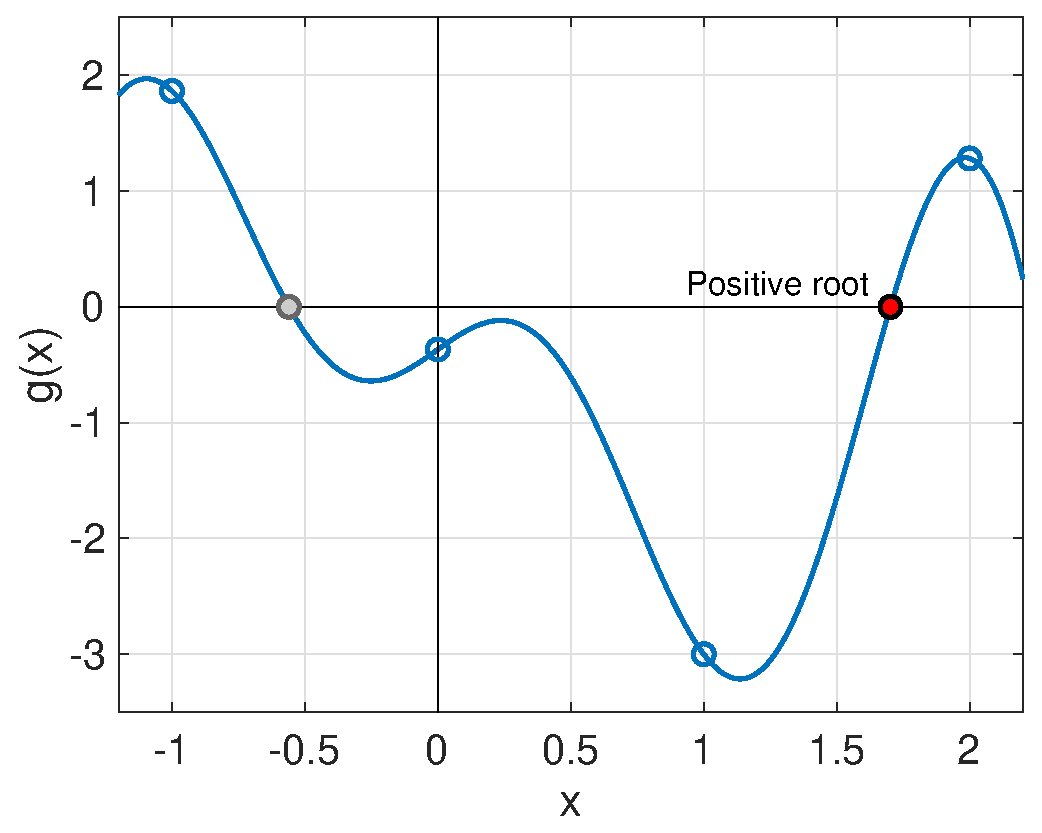
\includegraphics[width=0.4\textwidth]{figures/intbisect}
    \end{center}}{\jms}


  \qitemMCfour{%
    \mytwocol[0.4]{This partial code implements the bisection method for
      finding a root of the nonlinear equation $f(x) = 0$.  The \Matlab
      function {\tt f} computes the function values and you can assume
      that you start with an interval $[a,b]$ satisfying $f(a) \cdot
      f(b) < 0$. Select the suitable replacement code for the blanks
      marked \circnum{1} and \circnum{2} from the list below.}%
    {{\tt
        tol = 1e-6;   \% tolerance\\
        fa = f(a); fb = f(b); \\
        done = 0;\\
        while( (b-a)/2 > tol ),

        ~~~mid = (a+b)/2;
        
        ~~~fmid = f(mid);

        ~~~if fmid == 0, \% mid is a solution

        ~~~~~~break;

        ~~~end

        ~~~if sign(fmid)*sign(fa) < 0,

        ~~~~~~...\circnum{1}...

        ~~~else

        ~~~~~~...\circnum{2}...

        ~~~end

        end}
    }}%
  {{\tt ~~\circnum{1}~b=mid; fb=fmid; ~~\circnum{2}~a=mid; fa=fmid;}}%
  {{\tt ~~\circnum{1}~a=mid; fa=fmid; ~~\circnum{2}~b=mid; fb=fmid;}}%
  {{\tt ~~\circnum{1}~a=mid; fb=fmid; ~~\circnum{2}~b=mid; fa=fmid;}}%
  {{\tt ~~\circnum{1}~a=mid; ~~~~~~~~~~~\circnum{2}~b=mid;}}%
  {1}{}{\courseID midterm question (Fall 2018)} 
  
\end{clicklist} 

%%%%%%%%%%%%%%%%%%%%%%%%%%%%%%%%%%%%%%%%%%%%%%%%%%%%%%%%%%%%%%%%%%%%%%%%%%%%%%
\mysubhead{2b}{Fixed Point Method}

\begin{clicklist}

  \qitemMCfour{Consider the fixed point iteration $x_{k+1} = g(x_k)$
    with $\ds{g(x) = \frac{x}{3} + \frac{4}{3x}}$.  Which root-finding
    problem is this equivalent to?}%
  {$x^2 - 2 = 0$}%
  {$\ds{\frac{x}{3} + \frac{4}{3x}=0}$}%
  {$\ds{\frac{1}{3} - \frac{4}{3x^2} = 0}$}%
  {$\ds{x - \frac{1}{3} + \frac{4}{3x^2} = 0}$}%
  {1}{}{\mah}
  

  \qitemMCfour{Assuming that the following fixed point iteration
    converges 
    \begin{gather*}
      x_{k+1} = \half \left(x_k + \frac{3}{x_k}\right),
    \end{gather*}
    to which fixed point will it converge?}%
  {$\sqrt{3}$}%
  {$\sqrt{2}$}%
  {$\sqrt{5}$}%
  {none of the above}%
  {1}{}{\mah}

  
  \qitemMCfour{For which of the functions below is $x^*=\sqrt{5}$ a
    fixed point?}%
  {$\ds{g(x) = \frac{x}{\sqrt{5}}}$}%
  {$g(x) = \sqrt{5}\, x$}%
  {$g(x) = x^2 - 4x$}%
  {$\ds{g(x) = 1 + \frac{4}{x+1}}$}%
  {4}{}{\mah}

  
  \qitemMCfour{Which of the following is a suitable fixed point iteration
    for solving the equation $\cos(x) - x = 0$?
    \begin{IVlist}
    \item $x_{k+1} = \cos(x_k)$
    \item $x_{k+1} = \cos^{-1}(x_k)$
    \item $x_{k+1} = x_k + \tan(x_k)$
    %\item $\ds{x_{k+1} = x_k + \frac{\cos(x_k) - x_k}{\sin(x_k) + 1}}$
    \end{IVlist}}% 
  {I}%
  {I and II}%
  {I and III}%
  {I, II and III}%
  {2}{}{\mah}
  
  
  \qitemMCfour{%
    \mytwocol{The intersection points between the curves $y = x$ and $y
      = g(x)$ are $x = 0$ and $x = 4$, as shown in the plot.  Which of
      the statements below regarding the fixed point iteration $x_{k+1}
      = g(x_k)$ is TRUE?
      \begin{IVlist}
      \item If $x_0 = 2$ then $x_k$ converges to 4.
      \item If $x_0 = 1$ then $x_k$ converges to 0.
      \item If $x_0 = 6$ then $x_k$ converges to 4.
      \end{IVlist}}%
    {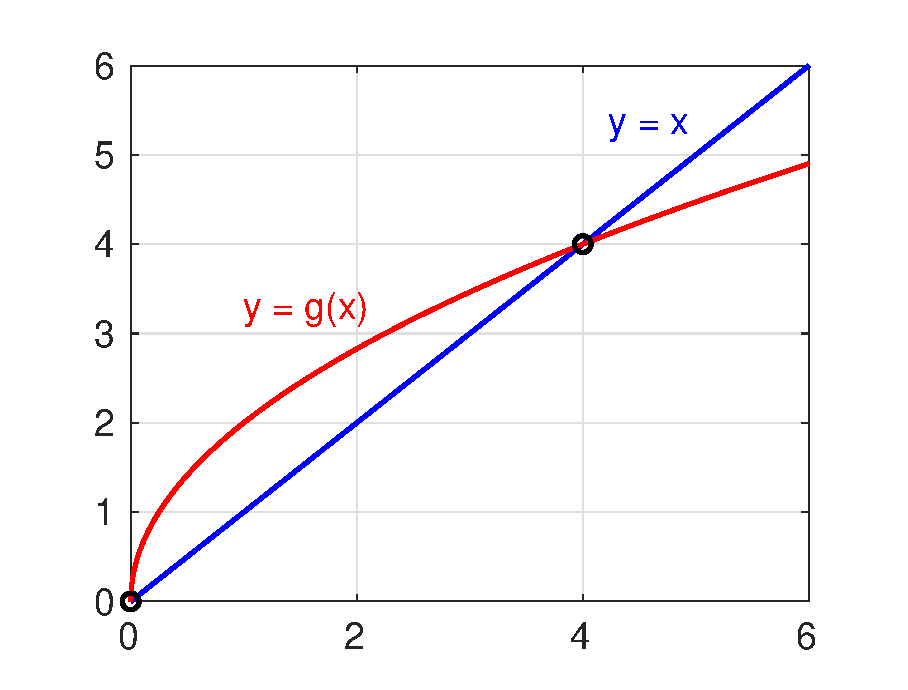
\includegraphics[width=\textwidth]{figures/fixiter}}}%
  {I and II}%
  {II and III}%
  {I and III}%
  {I, II and III}%
  {3}{}{\mah}
 

  \qitemMCfour{%
    \mytwocol{The intersection point between the curves $y = x$ and $y =
      g(x)$ is $x = x^*$, as shown in the plot.  Which of the statements
      below regarding the fixed point iteration $x_{k+1}=g(x_k)$ is
      TRUE?
      \begin{IVlist}
      \item Starting at $x_0 = 2$, the iteration converges to $x^*$.
      \item Starting at $x_0 = 1$, the iteration converges to $x^*$.
      \end{IVlist}}%
    {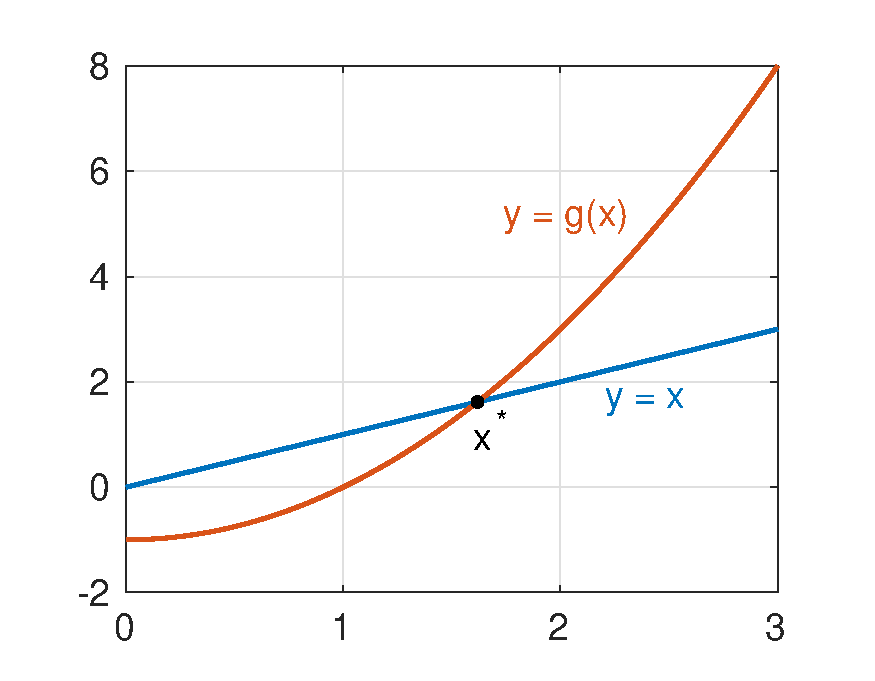
\includegraphics[width=\textwidth]{figures/fixiter2}}}%
  {I}%
  {II}%
  {I and II}%
  {Neither I nor II}%
  {4}{}{\mah}

  
  \qitemMCfour{Which of these statements is TRUE?
    \begin{IVlist}
    \item The fixed point and bisection methods have the same order of
      convergence. 
    \item If the iteration function $g(x)$ for the fixed point method
      satisfies $|g'(x)|<1$, then the fixed point algorithm converges
      faster than bisection.
    \item When it converges, the fixed point method always converges
      slower than bisection. 
    \end{IVlist}}% 
  {I and II}%
  {II and III}%
  {I and III}%
  {I, II and III}%
  {3}{Statement II is false in general, but could be true if
    $|g'(x)|<\half$ since then the asymptotic rate constant for
    the fixed point method is smaller than that of bisection.}{\jms,
    \courseID lecture notes}  


  \qitemMCfour{%
    \mytwocol[0.4]{This partial code implements the fixed point
      algorithm for finding a root of the equation $x = g(x)$, where the
      \Matlab function {\tt g} returns the value of the fixed point
      iteration function.  Select the best choice of terminating
      condition for this algorithm to fill in the missing condition in
      the {\tt if} statement.}%
    {{\tt
        tol = 1e-6;    \% tolerance\\        
        x = xguess;    \% initial guess\\
        done = 0;\\
        while( $\sim$done ),

        ~~~niter = niter + 1;

        ~~~x0 = x;

        ~~~x = g(x);

        ~~~if ...[fill in blank]...

        ~~~~~~done = 1;

        ~~~end\\
        end}}}%
  {{\tt abs(x) < tol}}%
  {{\tt abs(x - x0) < tol}}%
  {{\tt x - x0 < tol}}%
  {{\tt abs(g(x)) < tol}}%
  {2}{}{\courseID midterm question (Fall 2018)}
  
\end{clicklist} 

%%%%%%%%%%%%%%%%%%%%%%%%%%%%%%%%%%%%%%%%%%%%%%%%%%%%%%%%%%%%%%%%%%%%%%%%%%%%%% 
\mysubhead{2c}{Secant and Newton's Methods}

\begin{clicklist}

  \qitemMCfour{The irrational number $\sqrt{2}$ can be approximated by
    applying the secant method to the nonlinear equation $x^2-2=0$.
    What is the iteration formula?}%
  {$\ds{x_{k+1} = x_{k} - \frac{x_k^2 - 2}{x_k + x_{k-1}}}$}%
  {$\ds{x_{k+1} = x_{k} - \frac{(x_k^2 - 2)(x_k - x_{k-1})}{x_k +
        x_{k-1}}}$}%
  {$\ds{x_{k+1} = x_{k} - \frac{(x_k^2 - 2)(x_k - x_{k-1})}{x_k^2 +
        x_{k-1}^2}}$}%
  {$\ds{x_{k+1} = x_{k} - \frac{(x_k^2 - 2)(x_k - x_{k-1})}{x_k^2 -
        x_{k-1}^2 - 4}}$}%
  {1}{$\ds{x_{k+1} = x_{k} - \frac{f(x_k)(x_k - x_{k-1})}{f(x_k) -
        f(x_{k-1})} = x_{k} - \frac{(x_k^2 -2)(x_k - x_{k-1})}{x_k^2 -
        x_{k-1}^2} = x_{k} - \frac{x_k^2 - 2}{x_k + x_{k-1}}}$}{\mah}


  \qitemTF{The convergence of the secant method to simple roots is
    quadratic.}%
  {FALSE}{The convergence of the secant method to simple roots is
    superlinear, and lies between linear and quadratic convergence (the
    order of convergence is actually $p\approx 1.618$).}{\mah}

  
  \qitemTF{Both Newton's method and the secant method are examples of
    fixed-point iterations.}%
  {FALSE}{Newton's method is a fixed point iteration, but secant method
    is not.}{}

  
  \qitemMCfour{The irrational number $e$ can be approximated by applying
     Newton's method to solve the nonlinear equation $f(x) = \ln x - 1 =
     0$.  What is the Newton iteration formula?}%
  {$x_{k+1} = \ln x_k$}%
  {$x_{k+1} = x_{k} - \ln x_k$}%
  {$x_{k+1} = x_{k} - (\ln x_k - 1)$}%
  {$x_{k+1} = 2x_{k} - x_k \ln x_k$}%
  {4}{}{\mah}
  

  \qitemMCfive{The irrational number $\sqrt{2}$ can be approximated by
    applying Newton's method to the nonlinear equation $f(x) = x^2
    - 2 = 0$. What is the Newton iteration formula?}%
  {$\ds{x_{k+1} = x_k + \frac{x_k^2 - 2}{2x_k}}$}%
  {$\ds{x_{k+1} = x_k - \frac{x_k^2 - 2}{x_k}}$}%
  {$\ds{x_{k+1} = x_k - \frac{x_k^2 - 2}{x_k}}$}%
  {$\ds{x_{k+1} = x_k - \frac{x_k^2 - 2}{2x_k}}$}%
  {$\ds{x_{k+1} = \frac{x_k}{2} + \frac{1}{x_k}}$}%
  {4}{Response (E) is also correct, since it's just a simplified version
    of (D). \\[0.3cm]
    Indeed, (E) is a remarkably efficient formula that has been used to
    implement the square root operation on many modern floating-point
    processors!  Generalizing to the case of finding $\sqrt{c}$ as a
    root of $f(c)=x^2-c$, the Newton iteration is
    \begin{gather*}
      x_{k+1} = \frac{x_k}{2} + \frac{c}{2x_k} = \half \left(x_k + c\,
        \frac{1}{x_k} \right)
    \end{gather*}%
    Counting the flops involved, each iteration requires a reciprocal
    $(1/x_k)$, one multiplication by $c$, one addition, and one division
    by 2 (which is just a bit-shift in binary).  This is an incredibly
    cheap way to approximate $\sqrt{c}$ when the number of Newton
    iterations is small.}{\mah}
  
  
  \qitemMCfour{Apply Newton's method to the equation $f(x) = x^2 - 2 =
    0$ to estimate the root $x^* = \sqrt{2}$. Starting with the initial
    guess $x_0 = 1$, the first iteration $x_1$ is:}%
  {0.5}%
  {1.0}%
  {1.5}%
  {2.0}%
  {3}{The Newton iteration is $x_{1} = x_0 - \frac{x_0^2-2}{2x_0} =
    \frac{x_0}{2} + \frac{1}{x_0}$. Setting $x_0=1$ gives
    $x_1=\frac{3}{2}$.}{\mah} 
  
  \leavethisout{
    \qitemMCfour{The iteration formula for the method of false position,
      applied to finding a root of the equation $x^2 - 2 = 0$, is}% 
    {$x_{k+1} = x_{k} - (x_k^2 - 2)(x_k + x_{k-1})$}%
    {$x_{k+1} = x_{k} - (x_k^2 - 2)(x_k - x_{k-1})$}%
    {$x_{k+1} = x_{k} - \frac{x_k^2 - 2}{x_k + x_{k-1}}$}%
    {$x_{k+1} = x_{k} - \frac{x_k^2 - 2}{x_k - x_{k-1}}$}%
    {3}{}{\mah}
  }  
  

  \qitemMCfour{For which values of $x$ does Newton's method exhibit
    linear and quadratic order of convergence when applied to the
    function $f(x) = x(x-3)^2$\,?}%
  {linear near $x=0$ and quadratic near $x=3$}%
  {linear near $x=3$ and quadratic near $x=0$}%
  {linear convergence everywhere}%
  {quadratic convergence everywhere}%
  {2}{}{\mah}
  

  \qitemMCfour{Which of these statements is TRUE?
    \begin{IVlist}
    \item Newton's method may converge linearly
    \item Newton's method may converge quadratically
    \item Newton's method may not converge at all
    \end{IVlist}}%
  {none is true}%
  {I and II only}%
  {II and III only}%
  {I, II and III}%
  {4}{}{Heath~\cite{heath-2018}, Review Question 5.16, p.~246}
  

  \qitemMCfour{Which of these statements is TRUE?
    \begin{IVlist}
    \item Newton's method is guaranteed to converge
    \item Newton's method has a quadratic order of convergence
    \end{IVlist}}%
  {I}%
  {II}%
  {I and II}%
  {Neither I nor II}%
  {4}{}{\jms, \courseID lecture note}
  

  \qitemMCfour{The Newton iteration $\ds{x_{k+1} = x_k -
      \frac{f(x_k)}{f'(x_k)}}$ can be rewritten as a fixed point
    iteration
    \begin{gather*}
      x_{k+1} = g(x_k)~\textrm{where}~g(x) = x - \frac{f(x)}{f'(x)}.
    \end{gather*}
    Which of these statements is TRUE?
    \begin{IVlist}
    \item Newton's method fails when $f'(x_k) = 0$.
    \item The iteration converges if $|g'(x_k)|< 1$.
    \end{IVlist}}%
  {I}%
  {II}%
  {I and II}%
  {Neither I nor II}%
  {3}{}{\mah}
  

  \qitemMCfour{Which of these statements regarding the
    secant method is TRUE?
    \begin{IVlist}
    \item It is an example of a fixed-point iteration.
    \item It requires two initial guesses.
    \item No derivative calculation is needed.
    \end{IVlist}}%
  {I}%
  {I and II only}%
  {II and III only}%
  {I, II and III}%
  {3}{}{\jms, \courseID lecture notes}
  

  \qitemMCfour{%
    \mytwocol[0.4]{This partial code implements Newton's method for
      finding a root to the nonlinear equation $f(x) = 0$, where
      \Matlab functions {\tt f} and {\tt fprime} compute the function
      and its derivative. Select a suitable terminating condition (to
      replace the blank {\tt if} statement) that will best improve the
      robustness of the code.}%
    {{\tt 
        tol = 1e-6;   \% tolerance\\
        x = 2.0;      \% initial guess\\
        done = 0;\\
        while( $\sim$done ),
        
        ~~~xlast = x;
        
        ~~~fx = f(x);
        
        ~~~fpx = fprime(x);
        
        ~~~x = xlast - fx / fpx;
        
        ~~~if ...[fill in blank]...
        
        ~~~~~~done = 1;
        
        ~~~end\\        
        end}}}%
  {{\tt abs(x) < tol}}%
  {{\tt abs(x - xlast)/abs(x) < tol}}%
  {{\tt abs(fx) < tol}}%
  {{\tt abs(x - xlast)/abs(x) < tol \& abs(fx) < tol}}%
  {4}{}{\courseID midterm question (Fall 2018)} 
  

  \qitemMCfour{%
    \mytwocol[0.4]{This partial code implements the method of false
      position for finding a root of the nonlinear equation $f (x) = 0$,
      where the \Matlab function {\tt f} computes the function
      value. Provide suitable code to replace the blanks marked
      \circnum{1} and \circnum{2}.}%
    {{\tt 
        while( abs(x0-x1) > tol ),   \% absolute error tolerance 
        
        ~~~x2 = x1 - f(x1)*(x1-x0)/(f(x1)-f(x0));
        
        ~~~if f(x2)*f(x1) > 0,
        
        ~~~~~~...\circnum{1}...
        
        ~~~else
        
        ~~~~~~...\circnum{2}...
        
        ~~~end\\        
        end}}}%
  {{\tt~\circnum{1}~x1 = x2;~~\circnum{2}~x0 = x2;}}%
  {{\tt~\circnum{1}~x2 = x1;~~\circnum{2}~x2 = x0;}}%
  {{\tt~\circnum{1}~x0 = x2;~~\circnum{2}~x1 = x2;}}%
  {{\tt~\circnum{1}~x2 = x0;~~\circnum{2}~x2 = x1;}}%
  {1}{}{\courseID midterm question (Fall 2018)}  
  

  \leavethisout{
    \qitemMCfour{%
      \mytwocol[0.4]{This partial code implements the method of false
        position for finding a root to the nonlinear equation $f(x) =
        0$, where the \Matlab function {\tt f} computes the function
        value. The first two iterations are shown in the plot
        below. What will be the changes in {\tt if} statement for these
        two iterations?}%
      {{\tt 
        while( abs(x0-x1) > tol ),  \% absolute error tolerance \\
        
        ~~~x2 = x1 - f(x1)*(x1-x0)/(f(x1)-f(x0));
        
        ~~~if f(x2)*f(x1) > 0,
        
        ~~~~~~x1 = x2;
        
        ~~~else
        
        ~~~~~~x0 = x2;
        
        ~~~end\\        
        end}}
    \begin{center}
      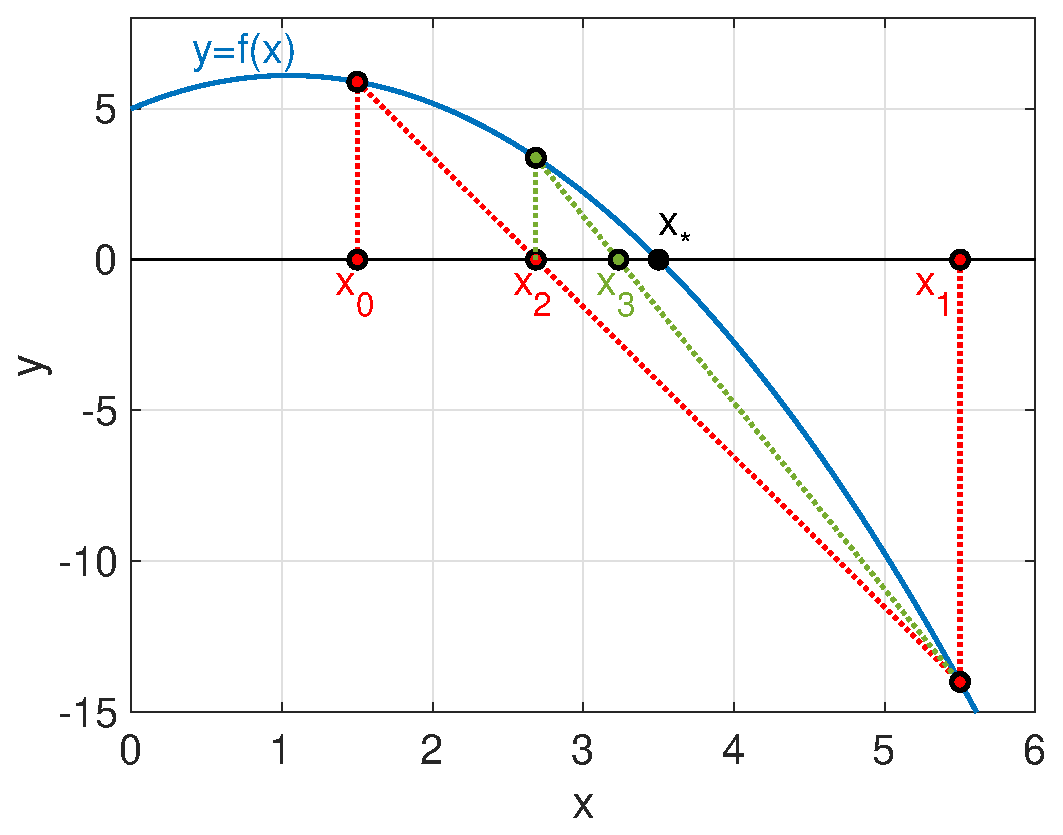
\includegraphics[width=0.45\textwidth]{figures/falsi}
    \end{center}}%
  {{\tt x1 = $x_2$; x1 = $x_3$;}}%
  {{\tt x0 = $x_2$; x0 = $x_3$;}}%
  {{\tt x2 = $x_0$; x3 = $x_0$;}}%
  {{\tt x0 = $x_2$; x1 = $x_3$;}}%
  {2}{}{Plot taken from \jms, \courseID lecture notes}
  }


  \qitemMCfour{After writing a \Matlab code that implements Newton's
    method, you apply it to the function $f(x)=2x^3-3x^2+4x-6$.  Using
    an initial guess of $x_0=1.5$, your code returns a result of ``{\tt
      -Inf}'' on the first iteration.  What is the most likely
    explanation for this behaviour?}%
  {$f(x)$ has a simple root at $x=1.5$.}%
  {$f(x)$ has a multiple root at $x=1.5$.}%
  {$f'(x)$ has a root at $x=1.5$.}%
  {Accumulation of round-off error due to subtractive cancellation.}%
  {3}{This one is a little bit tricky.  You need to look at the Newton
    iteration
    \begin{gather*}
      x_{k+1} = x_k - \frac{f(x_k)}{f'(x_k)}
    \end{gather*}
    and see there are two possible invalid floating point
    operations:
    \begin{itemize}
    \item $\pm${\tt Inf} or {``\,$\frac{1}{0}$''}: occurs if $f'(x_k)=0$
      and $f(x_k)\neq 0$. This is case (C).
    \item {\tt NaN} or ``\,$\frac{0}{0}$'': occurs if both $f'(x_k)=0$ and
      $f(x_k)=0$. This is response (B) -- a root with
      multiplicity 2.  
    \end{itemize}}{\jms}
  
  
  \qitemMCfour{Which of the following is an advantage of the secant
    method over Newton's method?}%
  {lower cost per iteration}%
  {faster convergence rate}%
  {more robust convergence far away from the solution}%
  {avoids computing the derivative}%
  %{all of the above}%
  {1}{The secant method only requires a single function evaluation in
    each step (as long as the previous value is saved), whereas the
    Newton iteration must compute values of both $f$ and $f'$ in every
    step.  This means that (D) is also
    correct.}{Heath~\cite{heath-2018}, Review Question 5.38, p.~247}


  \qitemMCfive{For the function $f(x)$ plotted below, use each of the
    four points $x_1$, $x_2$, $x_3$ and $x_4$ as the starting guess for
    Newton's method.  For which point(s) do you expect the iteration to
    converge to the root shown?
    \begin{center}
      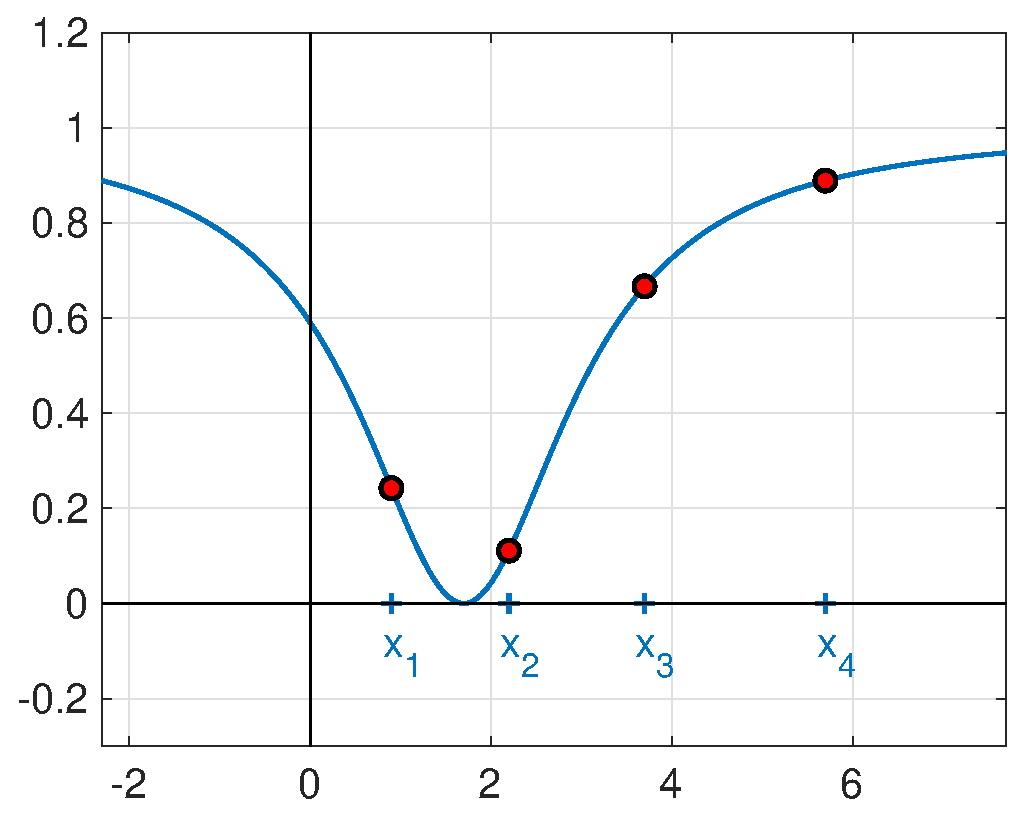
\includegraphics[width=0.45\textwidth]{figures/newton}
    \end{center}}%
  {$x_1$ and $x_2$ only}%
  {$x_2$ only}%
  {$x_1$, $x_2$ and $x_3$ only}%
  {All four points}%
  {none of the points}%
  {3}{Check by plotting the Newton iterations on the
    graph.}{GoodQuestions~\cite{goodquest-2019}, Newton's method}  
  
  
  \qitemMCfour{For the function $f(x)$ plotted below, use each of the
    intervals $[x_1,x_2]$, $[x_1, x_3]$ and $[x_1, x_4]$ as the starting
    guess for the secant method.  For which interval do you expect
    the iteration to converge to the root shown?
    \begin{center}
      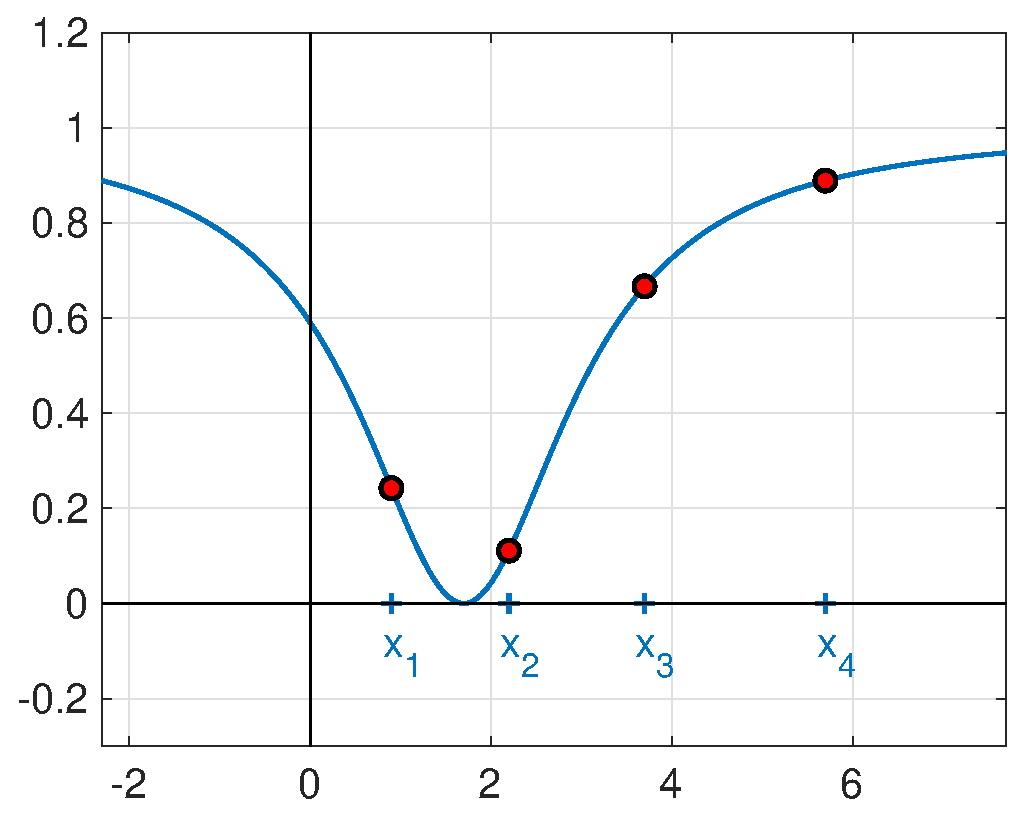
\includegraphics[width=0.45\textwidth]{figures/newton}
    \end{center}}%
  {$[x_1, x_2]$}%
  {$[x_1, x_3]$}%
  {$[x_1, x_4]$}%
  {none of the intervals}%
  {1}{Check by plotting the secant lines joining each pair of
    points.}{GoodQuestions~\cite{goodquest-2019}, Newton's method}
  
  
  \qitemMCthree{Let $f$ be a differentiable function that is defined for
    all $x$.  Starting Newton's method at a point $x_0$ where
    $f'(x_0)=0$ is \dots}%
  {a good choice, because $x=x_0$ is a critical point of $f$ and
    Newton's method will converge most rapidly to the root from there}%
  {a bad choice, because the Newton iteration fails}%
  {usually a bad choice, but it might work if we're lucky}%
  {2}{Strictly, (C) is also correct since it's possible we might have
    starting with an $x_0$ that is a root -- this is what is meant by
    ``lucky''. In every other case, the Newton iteration formula fails
    because of division by zero.}{GoodQuestions~\cite{goodquest-2019},
    Newton's method}
  

  \qitemMCfour{Newton's method is an appealing root-finding technique
    because \dots}%
  {it can be used to find quick and accurate approximations to radical
    numbers like $\sqrt[4]{3}$ or $\sqrt[8]{13}$}%
  {it can reliably determine all real roots of an $n^{th}$ degree
    polynomial}%
  {it can find a solution to $7x^8 + x^4 + 1 = 0$}%
  {it converges faster than other root-finding methods}%
  {1}{The radical expression $\sqrt[n]{a}$ is a root of $f(x)=x^n-a=0$,
    which can always be found with Newton's method (plot $f(x)$ to see
    why).  Response (B) is incorrect because Newton's method requires a
    good initial guess for each root, which can be difficult/impossible
    in practice.  Response (C) is incorrect because there is no real
    root (just rewrite as $7x^8=-1-x^4$, ``positive equals negative'').
    Response (D) is often true, but not
    always.}{GoodQuestions~\cite{goodquest-2019}, Newton's method}

\end{clicklist}

%%%%%%%%%%%%%%%%%%%%%%%%%%%%%%%%%%%%%%%%%%%%%%%%%%%%%%%%%%%%%%%%%%%%%%%%%%%%%%
\mysubhead{2d}{General Aspects of Convergence}

\begin{clicklist}
  
  \qitemMCfour{Suppose you apply an iterative method and obtain the
    following errors from the first four steps:
    \begin{gather*}
      10^{-2}, \; 10^{-4}, \; 10^{-6}, \; 10^{-8}, \;\dots
    \end{gather*}
    How would you characterize the order of convergence of this
    method?}%
  {linear}%
  {super-linear}%
  {quadratic}%
  {faster than quadratic}%
  {2}{The error $E_k$ is reduced by a factor of 100 in every iteration
    and so can be written $E_k = 10^{-2} E_{k-1}$.  According to the
    definition of convergence, this is linear (order 1) convergence with
    an asymptotic rate constant equal to
    $10^{-2}$.}{Heath~\cite{heath-2018}, adapted from Review Question
    5.9, p.~245} 

  
  \qitemMCfour{Suppose you apply an iterative method and obtain the
    following errors from the first four steps:
    \begin{gather*}
      10^{-2}, \; 10^{-4}, \; 10^{-8}, \; 10^{-16}, \; \dots
    \end{gather*}
    How would you characterize the order of convergence of this
    method?}%
  {linear}%
  {super-linear}%
  {quadratic}%
  {faster than quadratic}%
  {3}{The error $E_k$ is squared in every iteration and so can be
    written $E_k = E_{k-1}^2$.  According to the definition, this is
    quadratic (order 2) convergence with asymptotic rate constant equal
    to $1$.  Note that the response (B) is strictly also correct,
    although (C) is more precise.}{Heath~\cite{heath-2018}, adapted from
    Review Question 5.9, p.~245}


  \qitemMCfour{Suppose you apply an iterative method and obtain the
    following errors from the first six steps of an iterative method:
    \begin{gather*}
      0.01369, \; 0.02553, \; 0.01158, \; 0.01044, \; 0.009781, \;
      0.008235, \; \dots
    \end{gather*}
    How would you characterize the order of convergence of this
    method?}%
  {not converging}%
  {linear}%
  {quadratic}%
  {impossible to determine}%
  {1}{It's actually very hard to tell in this case, and it would be
    helpful if there were more iterations to based the decision on.  But
    we can make an educated guess.  At best, the method is converging
    very slowly, perhaps linear with a rate constant just slightly less
    than 1.  So (A), (B) and (D) are all reasonable responses.  The
    anomalous ``blip'' at the start can probably be ignored because
    convergence isn't always uniform.}{\jms}


  \qitemMCfour{If you have an iterative method that converges linearly
    with rate constant $\half$, how many iterations are required for the
    initial error to be reduced by a factor of at least 1000?}%
  {5}%
  {10}%
  {20}%
  {100}%
  {2}{The error from step $k$ obeys $E_k \leqslant \half E_{k-1}$
    $\Longrightarrow$ $E_k \leqslant (\half)^k E_0$.  This means that we
    need $\left(\half\right)^k \leqslant \frac{1}{1000} \;\;
    \Longrightarrow \;\; 2^k \geqslant 1000 \;\; \Longrightarrow \;\; k
    \geqslant \log_2(1000) \approx 9.97$.}{\jms}


  \qitemMCfour{If an iterative method approximately squares the error in
    every \myuline{two} iterations then what is its order of
    convergence?}%
  {0.5}%
  {1}%
  {$\sqrt{2}$}%
  {2}%
  {3}{We're given that the error in step $k$ satisfies $E_k \approx
    E_{k-2}^2$.  But from the definition of convergence for a method of
    order $p$, the error in step $k$ also satisfies $E_k \approx
    E_{k-1}^p \approx E_{k-2}^{p^2}$. Comparing these two expressions
    for $E_k$ suggests that $p^2=2$ or
    $p=\sqrt{2}$.}{Heath~\cite{heath-2018}, adapted from Review Question
    5.14, p.~246}


  \qitemMCfive{For some root finding method, you determine that the
    absolute error in step $k$ satisfies $E_k \leqslant 0.2 E_{k-1}^3$.
    Which of the statements below is TRUE?}%
  {The method is superlinearly convergent.}%
  {The order of the method is 0.2.}%
  {The asymptotic rate of convergence is $\log_{10}(0.2)$.}%
  {The iteration will always converge.}%
  {All of the above.}%
  {1}{Based on our definition of convergence, $\alpha=0.2$ is the
    asymptotic rate constant and the order of convergence is $p=3$
    (faster than linear).  Response (D) is not always true because the
    iteration may not converge if the initial guess has an error that
    satisfies $E_0>1$.}{\jms}


  \qitemMCfour{You use two different iterative methods to compute an
    approximation, and the errors from each method are plotted below
    versus the iteration number:
    \begin{center}
      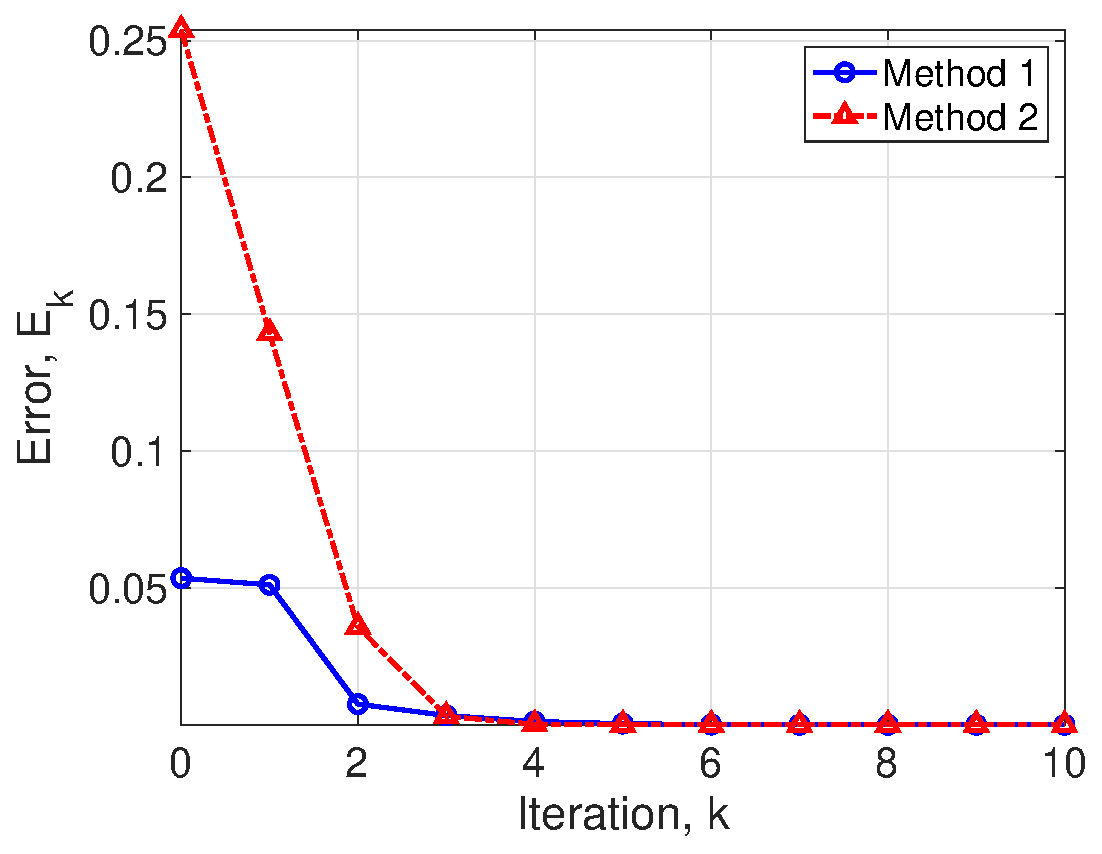
\includegraphics[width=0.45\textwidth]{figures/convplot1}
    \end{center}
    What can you conclude about the iterative convergence of the two
    methods?}%
  {Both methods converge quadratically, but Method 1 has a smaller rate
    constant.}%
  {The order of convergence for Method 1 is linear and Method 2 is
    quadratic.}%
  {Both methods converge faster than linear, but the order cannot be
    estimated.}% 
  {No conclusion is possible based on this plot.}%
  {4}{The order of convergence can't be estimated using this error plot
    with both axes having linear scales.  This is because the definition of
    convergence reads 
    \begin{gather*}
      E_k\leqslant \alpha E_{k-1}^p \quad \Longrightarrow \quad
      E_k\leqslant \alpha^k E_0^{p^k}
    \end{gather*}
  (for order $p$ and rate $\alpha$) which requires taking a logarithm of
  $E_k$ to reliably estimate either $p$ or $\alpha$.}{\jms}  
  

  \qitemMCfour{You use two different iterative methods to
    compute an approximation, and the errors from each method are
    plotted below versus the iteration number:
    \begin{center}
      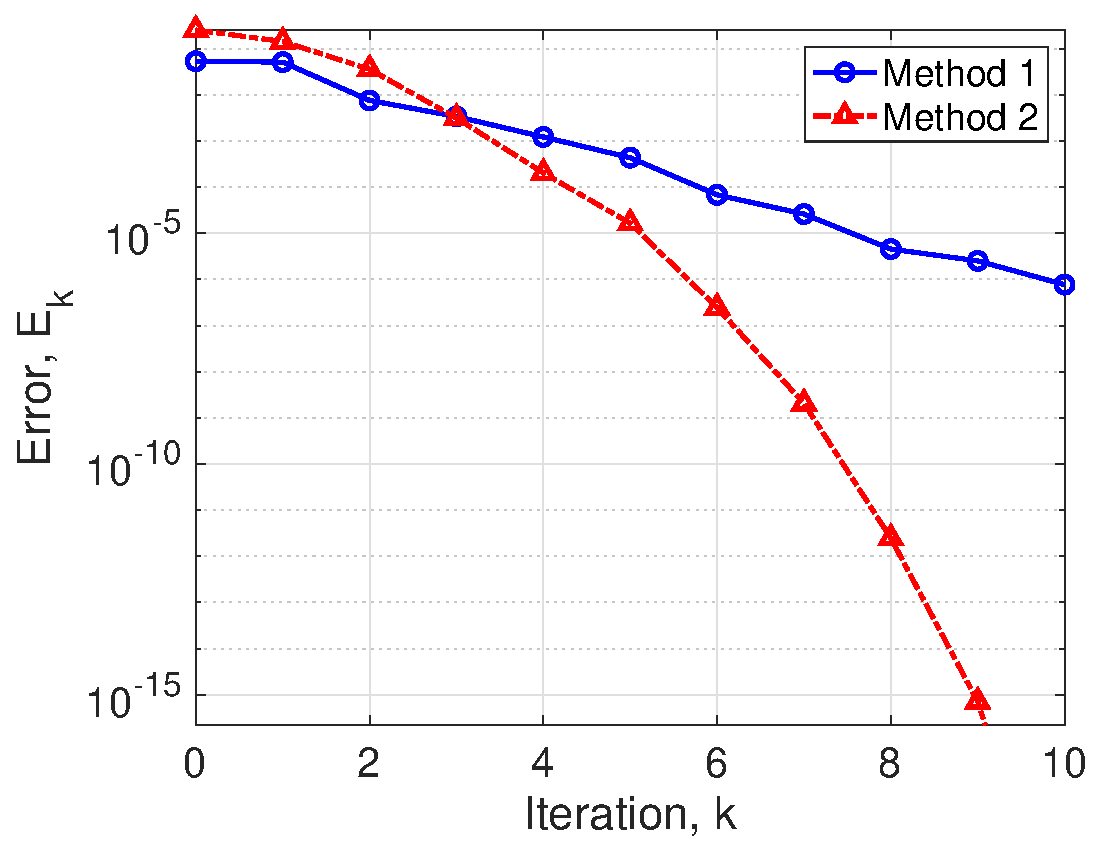
\includegraphics[width=0.45\textwidth]{figures/convplot1log}
    \end{center}
    What can you conclude about the iterative convergence of the two
    methods?}%
  {Both methods converge quadratically, but Method 1 has a smaller rate
    constant.}%
  {The order of convergence for Method 1 is linear and Method 2 is
    quadratic.}%
  {Method 1 converges linearly and Method 2 is super-linear.}%
  {No conclusion is possible based on this plot.}%
  {3}{The points from Method 1 appear to lie on a straight line.  Method
    2 curves downward so it's definitely superlinear.  It might converge
    quadratically but that's not possible to estimate from this semi-log
    plot.  Instead, you would have to plot $\log\log E_k$ (double-log)
    versus $k$.}{\jms} 

\end{clicklist}
  
%%%%%%%%%%%%%%%%%%%%%%%%%%%%%%%%%%%%%%%%%%%%%%%%%%%%%%%%%%%%%%%%%%%%%%%%%%%%%%
\mysubhead{2e}{Nonlinear Systems of Equations}

[~nothing here yet~]

%%%%%%%%%%%%%%%%%%%%%%%%%%%%%%%%%%%%%%%%%%%%%%%%%%%%%%%%%%%%%%%%%%%%%%%%%%%%%%
\newpage
\myhead{3}{Linear Systems of Equations}

\mysubhead{3a}{Review of Linear Algebra}

\begin{clicklist}

  \qitemMCfive{Which of the following properties of the matrix
    determinant is TRUE?}%
  {Only square matrices have a determinant}%
  {For the identity matrix, $\det(I) = 1$}%
  {$\det(AB) = \det(A) \det(B)$}%
  {$\det(A^T) = \det(A)$}%
  {All of the above}%
  {5}{}{\jms, \courseID lecture notes}
  
  
  \qitemMCfive{If $A$ is an invertible matrix then which of these
    statements is TRUE?}%
  {$\det(A) \ne 0$}%
  {$Ax = b$ has a unique solution for any vector $b$}%
  {$Ax = 0$ has only the trivial solution $x=0$}%
  {$A^T$ is invertible}%
  {All of the above}%
  {5}{}{\jms, \courseID lecture notes}

  
  \leavethisout{
    \qitemMCfour{If $\det(A) = 0$ then which of these statements TRUE?}%
    {$A$ has no inverse}%
    {There exist vectors $x \ne 0$ satisfying $Ax = 0$}%
    {Either $Ax = b$ has no solution or infinitely many solutions}%
    {All of the above}%
    {4}{}{\jms, \courseID lecture notes}
  }
  

  \leavethisout{
    \qitemMCthree{Which one of the following is true for the linear system
      $Ax = b$ where $A$ is an invertible matrix ?}%
    {$x = A^{-1}b$}%
    {$x = bA^{-1}$}%
    {Both (A) and (B)}%
    {1}{In order to solve $Ax = b$ for $x$, we must multiply by $A^{-1}$
      on the left, so we get $A^{-1}Ax = x = A^{-1}b$. }{\mah}
  }


  \leavethisout{
    \qitemMCfour{Suppose $A$ and $B$ are invertible matrics. If $AB = C$,
      then what is the inverse of $C$?}%
    {$A^{-1}B^{-1}$}%
    {$B^{-1}A^{-1}$}%
    {$A^{-1}B$}%
    {$AB^{-1}$}%
    {2}{$AB = C \implies A^{-1}AB = A^{-1}C \implies B = A^{-1}C$\\,
      $\implies B^{-1}B = B^{-1}A^{-1}C \implies I =
      B^{-1}A^{-1}C$. Therefore, $C^{-1} = B^{-1}A^{-1}$}{\mah}
  }
    

  \qitemTF{If a matrix $A$ is nonsingular then the number of solutions
    to the linear system $Ax=b$ depends on the particular choice of
    right hand side vector $b$.}%
  {FALSE}{There is a unique solution for any
    $b$.}{Heath~\cite{heath-2018}, Review Question 2.1, 
    p.~92}

  \qitemTF{If a triangular matrix has a zero entry on its main diagonal
    then the matrix must be singular.}%
  {TRUE}{The determinant of any triangular matrix is the product of the
    diagonal entries and so its determinant of this matrix is
    zero.}{Heath~\cite{heath-2018}, Review Question 2.3, p.~92}


  \qitemMCfour{If $A$ is a $5 \times 5$ matrix then what is the value of
    $\det(3A)$?}%
  {$\ds{\frac{1}{3^5} \det(A)}$}%
  {$\ds{\frac{1}{5^3} \det(A)}$}%
  {$\ds{3^5 \det(A)}$}%
  {$\ds{5^3 \det(A)}$}%
  {3}{}{\mah}


  \qitemMCfour{If $A$ is a $2 \times 2$ invertible matrix then what is
    the inverse of $2A$?}%
  {$\ds{\half A^{-1}}$}%
  {$\ds{\frac{1}{4}A^{-1}}$}%
  {$\ds{2A^{-1}}$}%
  {$\ds{4A^{-1}}$}%
  {1}{Notice that $2A \cdot \frac{1}{2}A^{-1} = AA^{-1} =
    I$.}{MathQuest~\cite{mathquest-2019}, Linear Algebra, Matrix
    Inverses}


  \qitemTF{$\|A\|_1 = \|A^T\|_\infty$.}%
  {TRUE}{The 1-norm is the maximum column sum, the $\infty$-norm is the
    maximum row sum, and the transpose ``flips'' the matrix so the
    columns turn into rows.}{Heath~\cite{heath-2018}, Review Question
    2.24, p.~93}


  \qitemMCfour{Which of the following is a reliable indicator that a
    matrix is nearly singular?}%
  {a small determinant}%
  {a small norm}%
  {a large norm}%
  {a large condition number}%
  {4}{Both (A) and (D) are acceptable answers, at least in exact
    arithmetic.  But floating-point calculations of determinants can
    lead to very large growth in round-off error, so the condition
    number tends to be a more reliable test.}{Heath~\cite{heath-2018},
    Review Question 2.62, p.~95}


  \qitemMCfive{Which of the following matrices is ill-conditioned?}%
  {$\begin{bmatrix} 10^{10} & 0 \\ 0 & 10^{-10} \end{bmatrix}$}%
  {$\begin{bmatrix} 10^{10} & 0 \\ 0 & 10^{10} \end{bmatrix}$}%
  {$\begin{bmatrix} 10^{-10} & 0 \\ 0 & 10^{-10} \end{bmatrix}$}%
  {$\begin{bmatrix} 1 & 2 \\ 2 & 4 \end{bmatrix}$}%
  {All of the above}%
  {1}{This matrix has condition number (in the 1-norm)
    \begin{gather*}
      \|A\|_1\cdot \|A^{-1}\|_1 = 
      \begin{Vmatrix} 10^{10} & 0 \\ 0 & 10^{-10} \end{Vmatrix}_1 \cdot
      \begin{Vmatrix} 10^{-10} & 0 \\ 0 & 10^{10} \end{Vmatrix}_1
      = 10^{10} \cdot 10^{10} = 10^{20} \;\; \text{(HUGE)}
    \end{gather*}
    But response (D) is also correct since that matrix is singular and so
    has condition number $\infty$.  The matrices in (B) and (C) are
    multiples of the identity matrix, so they are perfectly
    conditioned.}{Heath~\cite{heath-2018}, Review Question 2.61, p.~95}


  \qitemMCfour{You are given a system of equations containing a
    real parameter $a$:
    \begin{align*}
      2 x + 3 y &= 5\\
      4 x + a y &= 8
    \end{align*}
    Which of these statements is TRUE?}%
  {For $a = 6$, the system has no solution.}%
  {For $a = 6$, the system has infinitely many solutions.}%
  {The system has a unique solution for any real value of $a$.}%
  {The two lines intersect when $a=6$.}%
  {1}{}{\mah}

  
  \qitemMCfour{What are the eigenvalues of the matrix
    \begin{gather*}
      \begin{bmatrix}
        1 & 4 & 6 \\
        0 & 2 & 5 \\
        0 & 0 & 3
      \end{bmatrix} 
      \; \text{?}
    \end{gather*}}%
  {1, 2, 3}%
  {1, 4, 6}%
  {1, 0, 0}%
  {4, 5, 6}%
  {1}{}{\mah}

  
  \qitemMCfive{Which of the following matrices is strictly diagonally
    dominant, and hence invertible?
    \begin{gather*}
      \text{I.}\;\; \left[ \begin{array}{rrr} 
          -6 & 0 & 3 \\ 7 & 8 & -2 \\ 1 & -1 & 2
        \end{array} \right]
      \qquad
      \text{II.}\;\; \left[ \begin{array}{rrr} 
          -6 & 0 & 3 \\ 5 & 8 & -2 \\ 1 & -1 & 2
        \end{array} \right]
      \qquad
      \text{III.}\;\; \left[ \begin{array}{rrr} 
          -6 & 0 & 3 \\ 5 & 8 & -2 \\ 1 & -1 & 3
        \end{array} \right]
      \qquad
      \text{IV.}\;\; \left[ \begin{array}{rrr} 
          -6 & 0 & 3 \\ 1 & 2 & -2 \\ 1 & -1 & 8
        \end{array} \right]
      \qquad
    \end{gather*}}%
  {II}%
  {III}%
  {II and III}%
  {IV}%
  {All are strictly diagonally-dominant}%
  {1}{}{\jms}


  \qitemTF{It's a well-known fact that every strictly
    diagonally-dominant matrix is nonsingular.  Is it also true that
    every nonsingular matrix is strictly diagonally-dominant?}%
  {FALSE}{A simple counterexample is the matrix $A=\begin{bmatrix} 0 & 1
      \\ 1 & 0 \end{bmatrix}$ (the permuted identity matrix).  This is
    clearly invertible ($A^{-1}=A$) but not diagonally-dominant (DD).  This
    brings home an \myuline{important point}: checking for DD isa
    really easy test to determine whether a matrix is nonsingular, but
    it doesn't work for all nonsingular matrices (that is, some matrices
    that aren't DD can still be invertible, like $A$ above).}{\jms}


  \qitemMCfour{Find 
    $w = \left[ \begin{array}{r}
        -1 \\ 4 \\ 12
      \end{array} \right]$
    as a linear combination of
    $u = \left[ \begin{array}{r}
        -2 \\ 2 \\ 3
      \end{array} \right]$
    and
    $v = \left[ \begin{array}{r}
         1 \\ 0 \\ 2
      \end{array} \right]$.}%
  {$w = 2u + 3v$}%
  {$w = 2u - 3v$}%
  {$w = u + 3v$}%
  {$w = 2u + v$}%
  {1}{Check: $\left[ \begin{array}{r}
        -1 \\ 4 \\ 12
      \end{array} \right]
    = 2 \left[ \begin{array}{r}
        -2 \\ 2 \\ 3
      \end{array} \right]
    + 3 \left[ \begin{array}{r}
        1 \\ 0 \\ 2
      \end{array} \right]$.}{\mah}
  
  
  \qitemMCfourtwoc{Which of the graphs below represents the following
    system of equations?
    \begin{align*}
      x + 2y  &= 5\\
      2x + 4y &= 10
    \end{align*}}%
  {\begin{minipage}[t]{\textwidth} \vspace*{-10pt}
      \includegraphics[width=0.8\textwidth]{figures/linearsystem1}
    \end{minipage}}%
  {\begin{minipage}[t]{\textwidth}
      \vspace*{-10pt}
      \includegraphics[width=0.8\textwidth]{figures/linearsystem2}
    \end{minipage}}%
  {\begin{minipage}[t]{\textwidth}
      \vspace*{-10pt}
      \includegraphics[width=0.8\textwidth]{figures/linearsystem3}
    \end{minipage}}%
  {\begin{minipage}[t]{\textwidth}
      \vspace*{-10pt}
      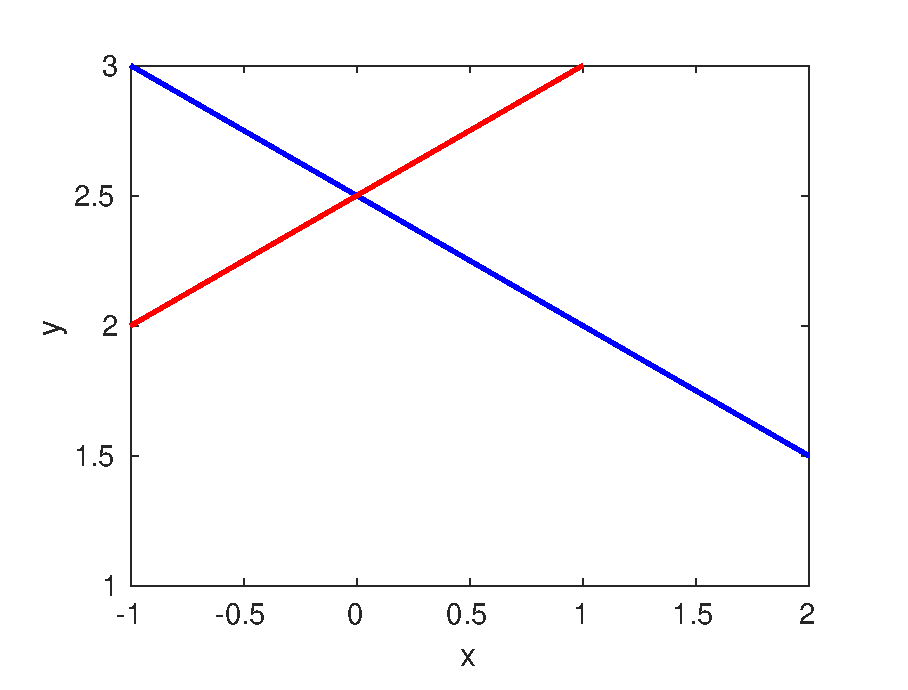
\includegraphics[width=0.8\textwidth]{figures/linearsystem4}
    \end{minipage}}%
  {2}{The second equation is simply the first multiplied by
    2, so these are just two equations for the same line (both with
    negative slope).}{\mah}
  

  \qitemMCfive{What is the solution to the following system of
    equations?
    \begin{align*}
      -3x + 6y  &= 3\\
      2x  - 4y  &= 4
    \end{align*}}%
  {$x=-1$ and $y=0$}%
  {$x=3$ and $y=2$}%
  {$x=3$ and $y=\frac{1}{2}$}%
  {There are no solutions}%
  {There are an infinite number of solutions}%
  {4}{The equations can be scaled to get $x - 2y=-1$ and $x-2y = 2$,
    which are inconsisent with each other.}{\jms}

  
  \qitemMCfour{%
    \mytwocol{Which of the following linear systems is depicted in the
      graph?}%
    {\includegraphics[width=\textwidth]{figures/linearsystem1}}}%
  {$x + 2y = 5, \quad 2x + 4y = 10$}%
  {$x + 2y = 5, \quad 2x + 4y = 8$}%
  {$x + 2y = 5, \quad 2x - 4y = 10$}%
  {$x - 2y = 5, \quad 2x + 4y = 8$}%
  {2}{Both lines in the plot have the same slope ($-\half$), so we need
    to choose between (A) and (B).  Option (A) gives two identical lines
    and so the correct answer must be (B).}{\mah}


  \qitemMCfour{%
    \mytwocol{A system of three linear equations in two unknowns is
      pictured in the plot.  How many solutions does this system have?}%
    {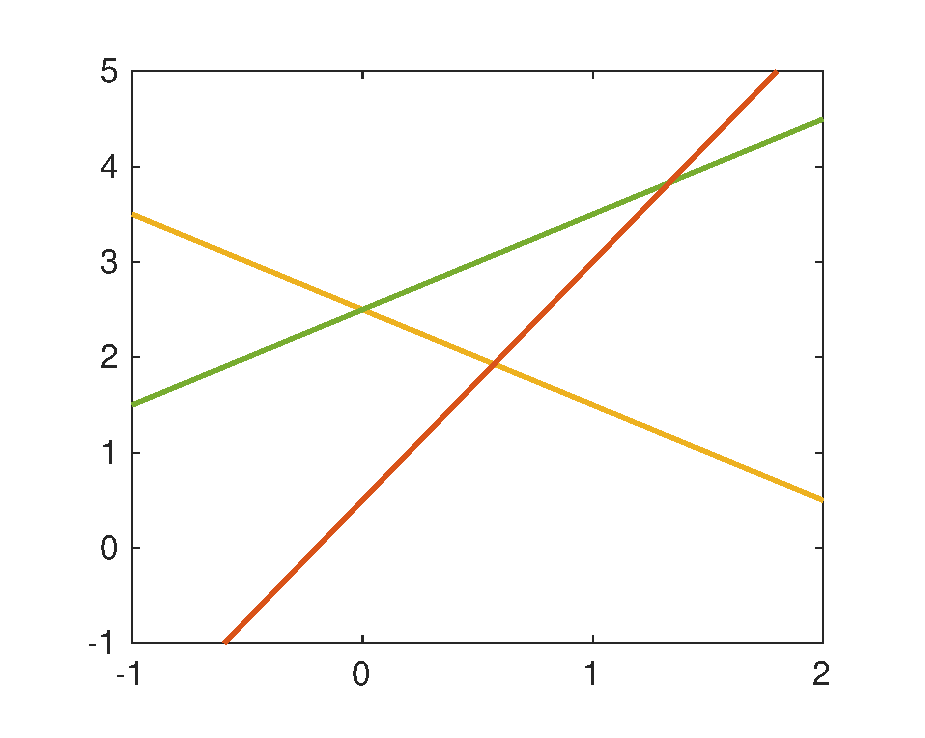
\includegraphics[width=1.0\textwidth]{figures/linearsystem5}}}%
  {0}%
  {1}%
  {3}%
  {Infinitely many}%
  {1}{There is no common intersection point and so this system has no
    solution.}{MathQuest~\cite{mathquest-2019}, Linear Algebra, Systems
    of Equations}
  

  \qitemTF{For any $n \times n$ matrix $A$, the equation $Ax=0$ has the
    unique solution $x=0$.}%
  {FALSE}{The equation $Ax = 0$ has $x=0$ as a unique solution if and
    only if $A$ is nonsingular, which is equivalent to saying that
    $A^{-1}$ exists or $\det(A)\ne 0$.}{\mah}


  \qitemMCfour{Suppose that both $A$ and $B$ are $n \times n$
    matrices. Which of the following statement is FALSE?}%
  {$\det(A+B) = \det(A) + \det(B)$}%
  {$\det(AB) = \det(A) \det(B)$}%
  {$\det(kA) = k^n\det(A)$}%
  {None of the above}%
  {1}{}{\mah}


  \qitemTF{If $A$ is any $n \times n$ nonsingular matrix, then $\cond(A)
    = \cond(A^{-1})$.}%
  {TRUE}{$\cond(A^{-1}) = ||A^{-1}||\cdot ||(A^{-1})^{-1}|| =
    ||A^{-1}||\cdot ||A|| = \cond(A)$}{{Heath~\cite{heath-2018}, Review
      Question 2.25, p.~93}}
          
\end{clicklist}

%%%%%%%%%%%%%%%%%%%%%%%%%%%%%%%%%%%%%%%%%%%%%%%%%%%%%%%%%%%%%%%%%%%%%%%%%%%%%%
\mysubhead{3b}{Gaussian Elimination and Pivoting}

\begin{clicklist}

  \qitemMCfour{\fillblank The goal of the row-reduction phase in the
    Gaussian elimination algorithm is to convert the coefficient matrix
    into a \mybigblank matrix.}%
  {diagonal}%
  {identity}%
  {lower triangular}%
  {upper triangular}%
  {4}{}{\jms}


  \qitemMCfour{If $A$ is a singular matrix, then which of the following
    statements is FALSE?}%
  {$\det(A) = 0$}%
  {A zero entry arises in the pivot position as Gaussian
    elimination with partial pivoting is applied to $A$}% 
  {$Ax = 0$ has only the trivial solution $x=0$}%
  {$\cond(A) = \infty$}%
  {2}{}{\jms}

  
  \qitemMCfour{When solving an upper or lower triangular system of size
    $n\times n$, the computational cost (measured in terms of
    multiplication and division operations) is roughly equal to \dots}%
  {$n^2$}%
  {$\half \,n^2$}%
  {$n^3$}%
  {$n$}%
  {1}{}{\jms}


  \qitemMCthree{Which of the following matrices CANNOT be obtained from 
    \begin{gather*}
      A = \begin{bmatrix} 
        2 & 1 & 3 & 1 \\ 0 & 1 & 3 & 4 \\ 1 & 2 & 0 & 4 
      \end{bmatrix}
    \end{gather*}
    using elementary row operations?}%
  {$\begin{bmatrix}
      2 & 4 & 0 & 8 \\ 0 & 1 & 3 & 4 \\ 2 & 1 & 3 & 1
    \end{bmatrix}$}%
  {$\begin{bmatrix}
      2 & 1 & 3 & 1 \\ 0 & 1 & 3 & 4 \\ 1 & 3 & 3 & 8
    \end{bmatrix}$}%
  {$\begin{bmatrix}
      1 & 2 & 3 & 1 \\ 1 & 0 & 3 & 4 \\ 2 & 1 & 0 & 4
    \end{bmatrix}$}%
  {3}{Response (A) results from $r_3 \leftarrow 2 r_3$ followed by the
    row swap $r_1 \leftrightarrow r_3$. Response (B) results from $r_3
    \leftarrow r_2 + r_3$. Response (C) involves a \myuline{column}
    swap.}{MathQuest~\cite{mathquest-2019}, Gaussian elimination}


  \qitemMCfour{Which of the following operations on an augmented matrix
    could change the solution of the corresponding linear system?}%
  {Interchanging two rows}%
  {Multiplying one row by any constant}%
  {Adding one row to another}%
  {None of the above}%
  {2}{Because every response seems to correspond to a row operation,
    it's very easy to make the mistake of choosing (D). However,
    response (B) could be an invalid row operation if the multiple is
    zero. So response (D) is only correct as long as it's understood
    that the constant multiple is
    non-zero.}{MathQuest~\cite{mathquest-2019}, Gaussian elimination}
  

  \qitemMCfive{What is the value of $\alpha$ so that the linear system
    represented by the following augmented matrix has infinitely many
    solutions?
    \begin{gather*}
      \left[\begin{array}{cc:c}
        2 & 6 & 8\\
        1 & \alpha & 4
      \end{array}\right]
    \end{gather*}}%
  {$\alpha=0$}%
  {$\alpha=2$}%
  {$\alpha=3$}%
  {$\alpha=4$}%
  {There is always a unique solution}%
  {3}{The two rows are linearly independent as long as $\alpha \neq 3$,
    in which case row 2 is multiple of row 1 and the system
    becomes underdetermined.}{MathQuest~\cite{mathquest-2019}, Gaussian
    elimination}
  
  
  \qitemMCfive{Let $R$ be the row-reduced echelon form of an $n\times n$
    matrix $A$.  Then \dots}%
  {$R$ is the identity}%
  {$R$ has at least one row of zeroes}%
  {Neither (A) nor (B)}%
  {Both (A) and (B)}%
  {The answer depends on the matrix $A$}
  {5}{}{MathQuest~\cite{mathquest-2019}, Gaussian
    elimination}
  
  
  \qitemMCfour{When solving a linear system of size $n\times n$ using
    Gaussian elimination with partial pivoting, the computational cost
    (measured in terms of multiplication and division operations) of the
    backward substitution step is \dots}%
  {$O(n)$}%
  {$O(n^{3/2})$}%
  {$O(n^2)$}%
  {$O(n^3)$}%
  {3}{}{\jms}


  \qitemMCfour{When computing the $LU$ factorization of an $n\times n$
    matrix, the computational cost (measured in terms of multiplication
    and division operations) is \dots}%
  {$O(n)$}%
  {$O(n^{3/2})$}%
  {$O(n^2)$}%
  {$O(n^3)$}%
  {4}{}{\jms}


  \qitemMCfour{The matrix $B$ is singular if \dots}%
  {$B$ is not square}%
  {Gaussian elimination with partial pivoting fails on $B$}%
  {$B$ is its own inverse}%
  {$B$ has no inverse}%
  {4}{}{\jms}


  \qitemMCfour{If you have to solve $Ax = b$ many times for different
    vectors $b$ but the same matrix $A$, it is best to \dots}%
  {compute the inverse of $A$}%
  {determine the $LU$ decomposition once, then apply forward/backward
    substitution for the different $b$'s}%
  {use an iterative method}%
  {use Gaussian elimination with partial pivoting}%
  {2}{}{\jms}


  \qitemTF{If a linear system is well-conditioned, then pivoting is
    unnecessary in Gaussian elimination.}%
  {FALSE}{A simple counterexample is given by the matrix
    \begin{gather*}
      A = \begin{bmatrix}
        0 & 1 & 0 \\ 1 & 0 & 0 \\ 0 & 0 & 1
      \end{bmatrix}
    \end{gather*}
    This is a permutation of the $3\times 3$ identity matrix so that $\cond(A) =
    1$, which is perfectly well-conditioned.  However, Gaussian
    elimination will fail without partial pivoting, because the first
    pivot element is $a_{11}=0$.}{Heath~\cite{heath-2018}, Review Question
    2.14, p.~92}

  
  \qitemMCthree{Consider the matrix
    \begin{gather*}
      A = \begin{bmatrix}
        4 &  -8 &  1 \\
        6 &   5 &  7 \\
        0 & -10 & -3
      \end{bmatrix} 
    \end{gather*}
    whose $LU$ factorization we want to compute using Gaussian
    elimination.  What will the initial pivot element be without
    pivoting, and with partial pivoting?}%
  {0 (no pivoting), \quad 6 (partial pivoting)}%
  {4 (no pivoting), \quad 0 (partial pivoting)}%
  {4 (no pivoting), \quad 6 (partial pivoting)}%
  {3}{}{Heath~\cite{heath-2018}, adapted from Review Question
    2.39, p.~93}
    

  \qitemMCfour{You have a system of three linear equations with three
    unknowns. If you perform Gaussian elimination and obtain the
    row-reduced echelon form
    \begin{gather*}
      \left[ \begin{array}{rrr:r}
          1 & -2 & 4 &  6 \\
          0 &  1 & 0 & -3 \\
          0 &  0 & 3 &  0  
        \end{array} \right]
    \end{gather*}
    then the system has \dots}%
  {a unique solution}%
  {no solution}%
  {infinitely many solutions}%
  {more than one solution}%
  {1}{The row-reduced matrix is upper triangular with nonzero
    diagonal entries.}{\mah}

  
  \qitemMCfour{You have a system of three linear equations with three
    unknowns. If you perform Gaussian elimination and obtain the
    row-reduced echelon form 
    \begin{gather*}
      \left[ \begin{array}{rrr:r}
          1 & -2 & 4 &  6 \\
          0 &  1 & 0 & -3 \\
          0 &  0 & 0 &  3  
        \end{array} \right]
    \end{gather*}
    then the system has \dots}%
  {a unique solution}%
  {no solution}%
  {infinitely many solutions}%
  {more than one solution}%
  {2}{The last equation reads ``\,$0=3$'' which is a
    contradiction.}{\mah} 


\newpage
  \qitemMCfour{You have a system of three linear equations with three
    unknowns. If you perform Gaussian elimination and obtain the
    reduced row echelon form
    \begin{gather*}
      \left[ \begin{array}{rrr:r}
          1 & -2 & 4 &  6 \\
          0 &  1 & 0 & -3 \\
          0 &  0 & 0 &  0  
        \end{array} \right]      
    \end{gather*}
    then the system has \dots}%
  {no solution}%
  {a unique solution}%
  {more than one solution}%
  {infinitely many solutions}%
  {4}{The last equation reads ``\,$0=0$'' so $x_3$ can be any real
    number. Strictly (C) is also correct, but (D) is the most accurate
    answer.}{\mah}   

  
  \qitemMCfive{Suppose that a square matrix $A$ is perfectly
    well-conditioned, meaning that $\cond(A)=1$.  Which of the following
    matrices shares this same property?}%
  {$cA$ where $c$ is any nonzero scalar}%
  {$DA$ where $D$ is any nonsingular diagonal matrix}%
  {$PA$ where $P$ is any permutation matrix}%
  {$A^{-1}$, the inverse of $A$}%
  {$A^T$, the transpose of $A$}%
  {1}{In fact, all of the responses are
    correct.}{Heath~\cite{heath-2018}, Review Question 2.58, p.~94} 


  \qitemTF{Every nonsingular $n \times n$ matrix $A$ can be written as a
    product $A=LU$.}%
  {FALSE}{For example, $A = \begin{bmatrix} 0 & 1 \\ 1 &
      1 \end{bmatrix}$ is nonsingular because $\det(A)=-1\neq 0$.  Any
    $LU$ factorization of $A$ must have the form 
    \begin{gather*}
      \begin{bmatrix} 0 & 1
        \\ 1 & 1 \end{bmatrix} = \begin{bmatrix} 1 & 0 \\ a &
        1 \end{bmatrix} \begin{bmatrix} b & c \\ 0 & d \end{bmatrix}
      = \begin{bmatrix} b & c \\ ab & ac + d \end{bmatrix}.
    \end{gather*}
    Equating coefficients in the first column yields $b=0$ and $ab=1$,
    which has no solution.  So this $A$ has no LU decomposition even
    though it's nonsingular. A simpler way to recognize this is that
    very first step of the LU algorithm fails when it encounters a zero
    in the $1,1$ pivot entry.}{\mah}


  \qitemMCfour{If $A = PI$ is some permutation $P$ of the identity
    matrix, then Gaussian elimination yields the following $L$ and $U$
    factors:}%
  {$L = U = I$}%
  {$L = U = PI$}%
  {$L = I$,~~$U = 0$}%
  {The factors depend on the permutation matrix $P$}%
  {1}{If $P$ is a permutation matrix then its inverse is another
    permutation matrix, $P^{-1} = \widetilde{P}$, and so $\widetilde{P}
    A = I$. This is already in row-reduced form, and so GE with partial
    pivoting yields the LU factorization of the same matrix
    $\widetilde{P}A=LU=I$. The factors are clearly $L = U =
    I$.}{\jms}


  \qitemTF{The $LU$ factorization is unique, so the output from the
    following \Matlab\ code must mean that there is a bug in the
    built-in function ``{\tt lu}'':\\ 
    {\tt >> L = [1 0 0; 2 1 0; 3 1 1];

         >> U = [2 0 1; 0 2 1; 0 0 2];

         >> [L2, U2] = lu(L*U)\\

         L2 = 0.3333~~-1.0000~~~1.0000

         ~~~~~0.6667~~~1.0000~~~0

         ~~~~~1.0000~~~0~~~~~~~~0\\

         U2 = 6.0000~~~2.0000~~~6.0000

         ~~~~~0~~~~~~~~0.6667~~-1.0000
         
         ~~~~~0~~~~~~~~0~~~~~~~-2.0000}}%
     {FALSE}%
     {The LU decomposition computed by \Matlab\ involves at least one
       row swap, so that the L and U factors are different.}{\jms}


  \qitemMCfour{You perform Gaussian elimination with partial pivoting to
    solve a linear system on a single-precision floating point computer
    with roughly 7 decimal digits of accuracy.  If the coefficient
    matrix has a condition number of $10^3$ and the the matrix and right
    hand side are both measured to within full machine precision, about
    how many digits of accuracy would you expect in the approximate
    solution?}%
  {2}%
  {3}%
  {4}%
  {7}%
  {3}{The error estimate tells us that $\left(\begin{array}{c}
        \text{relative}\\ \text{error} \end{array}\right) \leqslant
    \left(\begin{array}{c} \text{condition}\\
        \text{number} \end{array}\right) \cdot \left(\begin{array}{c}
        \text{error}\\ \text{in data} \end{array}\right) \leqslant
    10^{-7} \cdot 10^3 = 10^{-4}$, which corresponds to 4 decimal
    digits.  This is why we compute in
    double precision!!}{Heath~\cite{heath-2018}, Review Question 2.64,
    p.~95} 


  \qitemMCfour{Suppose you are solving a linear system $Ax=b$ on a
    computer with 12 decimal digits of floating-point precision, and
    that the matrix and right hand side are correct to within full
    machine precision.  Roughly how large can the condition number of
    the matrix $A$ be before the computed solution $x$ contains NO
    significant digits?}%
  {$10^{10}$}%
  {$10^{12}$}%
  {$10^{16}$}%
  {$10^{22}$}%
  {2}{The error estimate tells us that $\frac{\|x-\hat{x}\|}{\|x\|}
    \leqslant \cond(A) \, \frac{\|r\|}{\|b\|}$.  If the relative
    solution error is $O(1)=O(10^{0})$ (no digits of accuracy) and the
    ``data error'' (${\|r\|}/{\|b\|}$) is $O(\epsM)\approx 10^{-12}$,
    then the condition number must be
    $O(10^{12})$.}{Heath~\cite{heath-2018}, Review Question 2.65, p.~95}

  
  \qitemMCfour{You have a system of linear equations $Ax=b$ with
    $\|A\|=250$ and $\|A^{-1}\|=40$ that you solve using Gaussian
    elimination on a computer with machine epsilon $\epsM=1.19\times
    10^{-7}$.  What is the largest number of significant digits that you
    can trust in the solution?}%
  {1}%
  {2}%
  {3}%
  {4}%
  {4}{}{Holistic Numerical Methods~\cite{kaw-2019}}


  \qitemMCfour{You have a $100\times 100$ matrix $A$ and your computer
    is able to solve the linear system $Ax=b$ in exactly one minute
    using the LU factorization.  Roughly how much of that minute is
    spent computing the factorization $A=LU$?}%
  {30 secs}%
  {45 secs}%
  {53 secs}%
  {59 secs}%
  {4}{From the lecture notes, the ratio of time spent on the
    row-reduction to the total is
    \begin{gather*}
      \frac{{\cal R}(n)}{{\cal T}(n)} 
    = \frac{2n^3 + 3n^2 - {5n}}{2n^3 + 6 n^2 - {2n}}
    \approx \frac{2 + \frac{3}{n}}{2 + \frac{6}{n}}
    \end{gather*}
    When $n=100$ this ratio is $\frac{2.03}{2.06}\approx 0.99$
    which corresponds to roughly 59 seconds.}{\jms}


  \qitemMCfour{Suppose that your computer can solve 100 problems of the
    form $Ux=c$ in 1 second, where $U$ is a $50\times 50$ upper
    triangular matrix. Roughly how long will it take to solve a single
    $500\times 500$ problem of the form $Ax=b$ where $A$ is a full
    matrix?}%
  {10 seconds}%
  {1 minute}%
  {5 minutes, 30 seconds}%
  {5 hours}%
  {3}{The cost of solving $Ux=c$ is a backward substitution, which we
    know has cost with leading order term $\frac{n^2}{2}$ so the total
    cost is $\frac{100 (50^2)}{2} = 50^3$.  The full system has cost
    $\frac{n^3}{3}=\frac{500^3}{3}$ which is a fraction $\frac{1000}{3}$
    larger.  That translates into about 333 seconds.  A rough order of
    magnitude estimate (missing the constants) yields a ratio of
    $\frac{500^3}{100\cdot 50^2}=500$, and so choice (C) is still the
    closest answer.}{\jms}

\end{clicklist}

%%%%%%%%%%%%%%%%%%%%%%%%%%%%%%%%%%%%%%%%%%%%%%%%%%%%%%%%%%%%%%%%%%%%%%%%%%%%%%
\mysubhead{3c}{Plotting Power Laws}

\begin{clicklist}

  \qitemMCfour{%
    \mytwocol{A function is approximated near some given point $x_0$
      using two Taylor polynomials, $P_A(x)$ and $P_B(x)$.  On the right
      is a plot of the absolute error in these two polynomials as a
      function of $h$, where both are evaluated at the nearby point
      $x_0+h$.  What is the degree of the two Taylor polynomials?}%
    {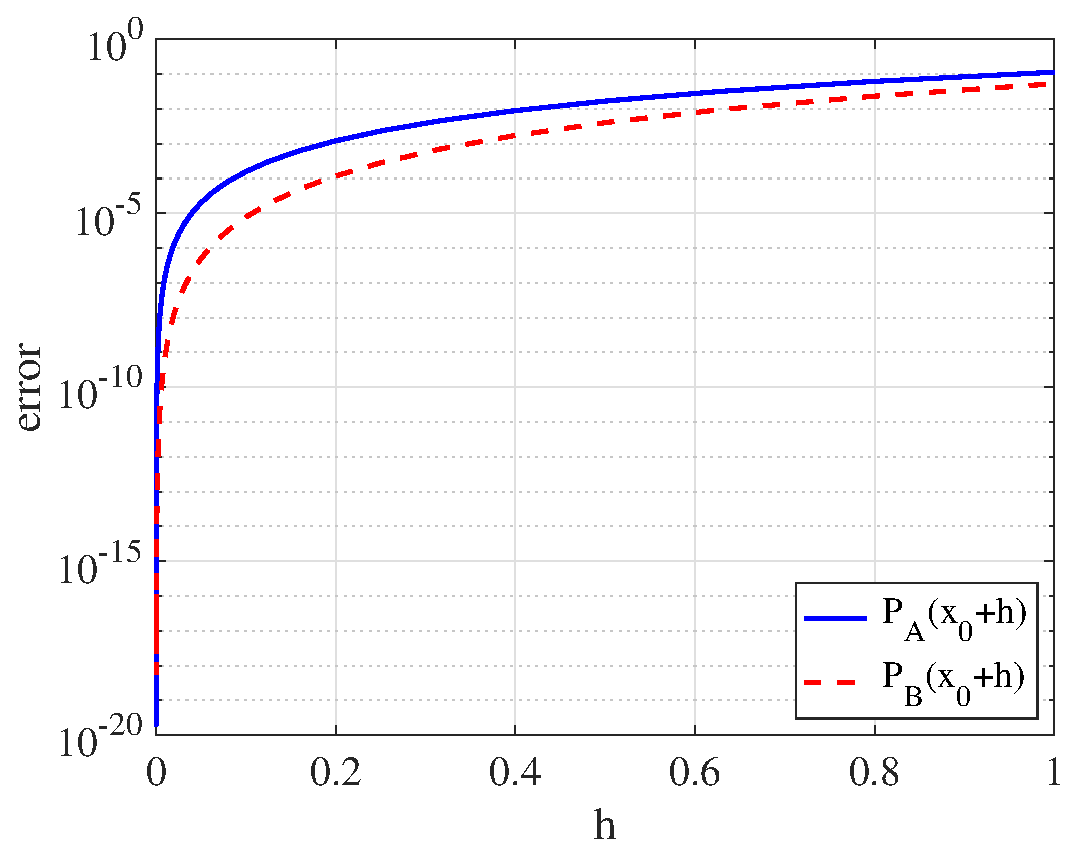
\includegraphics[width=\textwidth]{figures/powerlaw1a}}}%
  {$P_A$ is degree 2, $P_B$ is degree 3}%
  {$P_A$ is degree 3, $P_B$ is degree 4}%
  {$P_A$ and $P_B$ are both degree 3}%
  {The degree cannot be determined from this plot}%
  {4}{The remainder/error term for a Taylor polynomial of degree n takes
    the form
    \begin{gather*}
      R_n = \frac{f^{(n+1)}(c)}{(n+1)!}\, h^{n+1} 
      \quad \Longrightarrow \quad \log{R_n} \sim (n+1)\log h + \text{constant}
    \end{gather*}
    and so the degree can only be determined by plotting the data on a
    log-log scale.  This is a semi-log plot and so the nature of the
    polynomials can't be determined.}{\jms} 
  
  
  \qitemMCfour{%
    \mytwocol{A function is approximated near some given point $x_0$
      using two Taylor polynomials, $P_A(x)$ and $P_B(x)$.  On the right
      is a plot of the absolute error in these two polynomials as a
      function of $h$, where both are evaluated at the nearby point
      $x_0+h$.  What is the degree of the two Taylor polynomials?}%
    {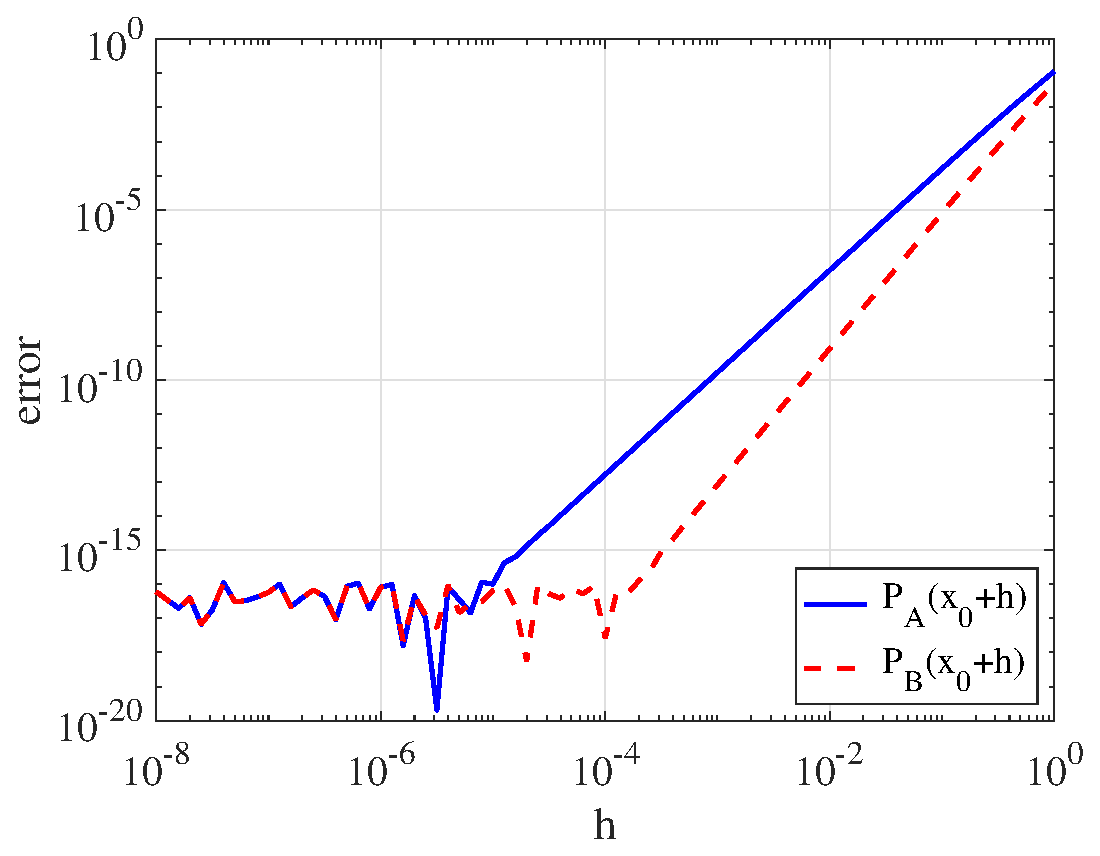
\includegraphics[width=\textwidth]{figures/powerlaw1b}}}%
  {$P_A$ is degree 2, $P_B$ is degree 3}%
  {$P_A$ is degree 3, $P_B$ is degree 4}%
  {$P_A$ and $P_B$ are both degree 3}%
  {The degree cannot be determined from this plot}%
  {1}{The remainder/error term for a Taylor polynomial of degree n takes
    the form
    \begin{gather*}
      R_n = \frac{f^{(n+1)}(c)}{(n+1)!}\, h^{n+1} 
      \quad \Longrightarrow \quad \log{R_n} \sim (n+1)\log h + \text{constant}
    \end{gather*}
    On this log-log plot, the errors behave linearly with slopes 3 and
    4, for $P_A$ and $P_B$ respectively.  The slope is $n+1$, one more
    than the degree.\\[0.5cm]
    Notice the oscillations appearing on the left half of the plot for
    small $h$ -- these are due to floating-point round-off error that
    dominates when the truncation error in the Taylor polynomials
    approaches the value of machine epsilon $\epsM \approx 2\times
    10^{-16}$.}{\jms} 

  \qitemMCthree{%
    \mytwocol{A function is approximated with Taylor polynomials of
      degrees 1 through 25, and the error in each approximation is
      plotted against the degree $N$ of the polynomial.  What happens
      when $N\gtrapprox 18$?}%
    {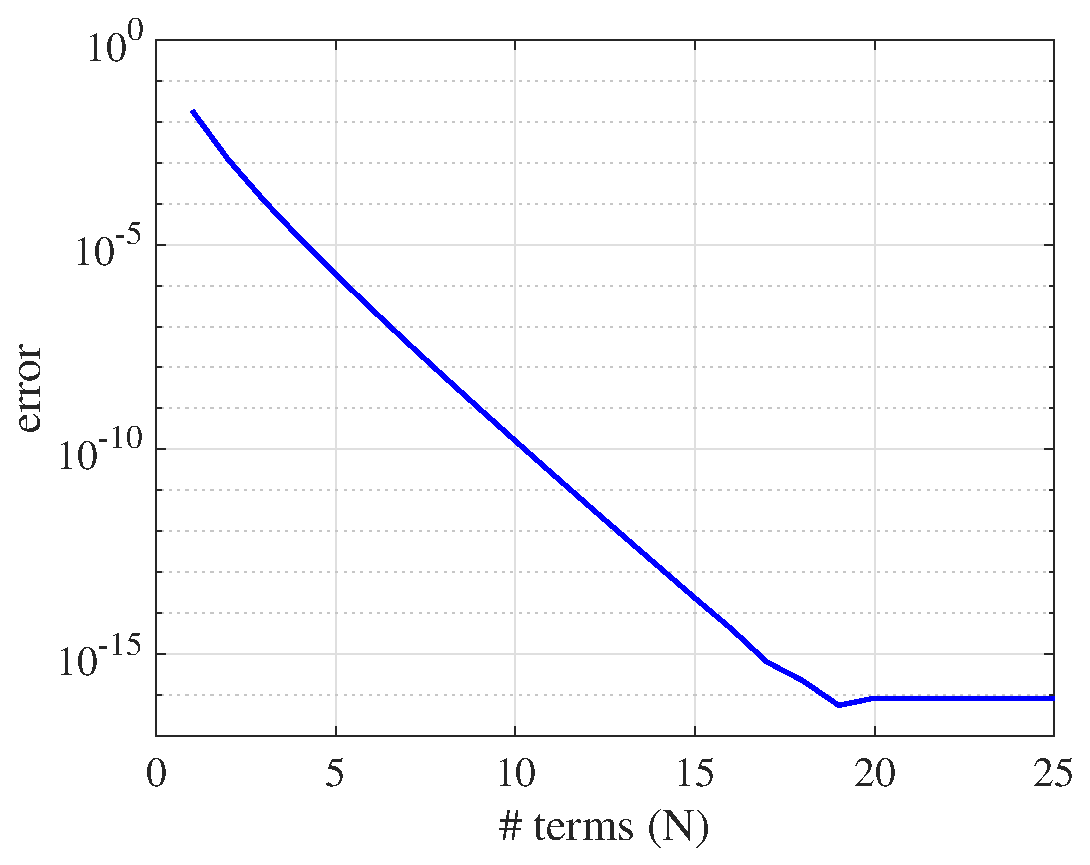
\includegraphics[width=\textwidth]{figures/powerlaw1c}}}%
  {The Taylor remainder term blows up when $N$ gets too large.}%
  {The accuracy is limited by the floating point machine epsilon.}%
  {Subtractive cancellation errors dominate when too many terms of
    differing signs are added to the polynomial.}%
  {2}{As $N$ increases, the error in the Taylor approximation gets
    smaller until it reaches machine epsilon, $\epsM\approx 2\times
    10^{-16}$, after which no more improvement in accuracy is possible.   
    This is not really a question about power laws, but the semi-log plot does
    clearly illustrate the linear dependence of error on $N$ (for fixed
    $h$) that we expect from:  
    \begin{gather*}
      R_N(h) = \frac{f^{(N+1)}(c)}{(N+1)!}\, h^{N+1} 
      \quad \Longrightarrow \quad \log{R_N} \sim (N+1)\log h + \text{constant}
    \end{gather*}}{\jms}


  \qitemMCthree{%
    \mytwocol{Suppose you are comparing three different algorithms and
      you use all three to solve the same problem for increasing values
      of problem size $N$. A plot of the CPU time required for each
      algorithm is shown on the right.  Which algorithm has a
      cost that scales as $O(N^{3/2})$?}%
    {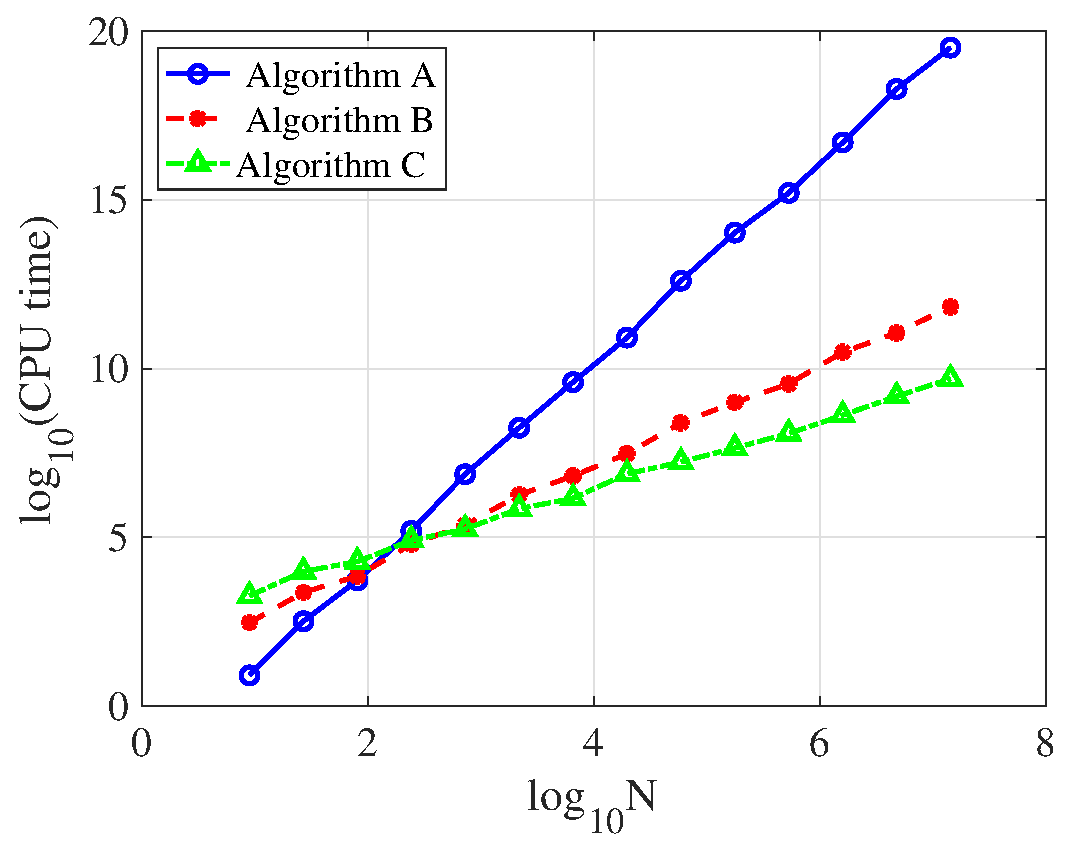
\includegraphics[width=\textwidth]{figures/powerlaw3a}}}%
  {Algorithm A}%
  {Algorithm B}%
  {Algorithm C}%
  {2}{This plot has a log-log scale.  If cost scales like $C = \alpha
    N^{3/2}$, then $\log C=\log \alpha  + \frac{3}{2}\, \log N$. So we are
    looking for the straight line with slope $\frac{3}{2}$, which is
    (B).}{\jms}
  

  \qitemMCfour{%
    \mytwocol{You have a code that you are using to compute several
      problems of increasing size $N$.  A plot of the CPU time required for
      each computation is shown on the right.  What is the best estimate
      of the leading-order cost of your algorithm as a function of $N$?}% 
    {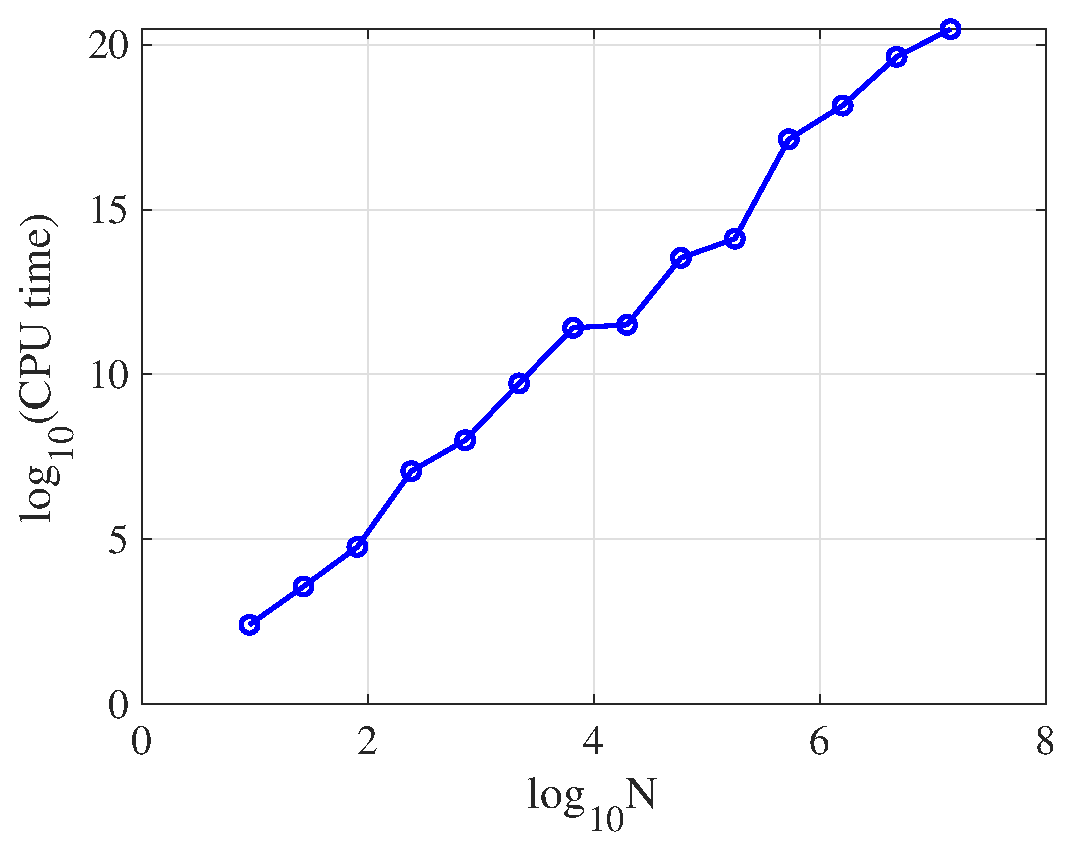
\includegraphics[width=\textwidth]{figures/powerlaw3bsave}}}%
  {$O(N)$}%
  {$O(N^{3/2})$}%
  {$O(N^{2})$}%
  {$O(N^{3})$}%
  {4}{This plot has a log-log scale.  If cost scales like $C = \alpha
    N^{p}$, then $\log C=\log \alpha + p \log N$ and should appear as a
    straight line with slope $p$. The plotted curve is roughly a
    straight line with slope $\approx\,\frac{20-2}{7-1}=3$.}{\jms}  
  

  \qitemMCfive{You write a code for an iterative algorithm that you
    believe converges quadratically.  To test whether you have
    implemented the algorithm correctly, you plot the relative error in
    each step, $R_k={|x_k-x^\ast|}/{|x^\ast|}$, as a function of the
    iteration number $k$.  Using which type of plot is it easiest to
    recognize the quadratic convergence?}%
  {A linear plot showing $R_k$ versus $k$.}%
  {A semi-log plot showing $\log R_k$ versus $k$.}%
  {A semi-log plot showing $R_k$ versus $\log k$.}%
  {A log-log plot showing $\log R_k$ versus $\log k$.}%
  {A double-log plot showing $\log(\log R_k)$ versus $k$.}%
  {5}{Because the error in a quadratic method behaves like $R_k \sim
    R_0^{2^k}$, then $\log R_k \sim (const)\cdot 2^k$ and $\log(\log
    R_k) \sim (const)\cdot k$. It is easiest to recognize a straight
    line and so you should plot $\log(\log R_k)$ versus $k$.}{\jms}


  \qitemMCfour{You write a code for an iterative algorithm that you
    believe converges superlinearly.  To test whether you have
    implemented the algorithm correctly, you plot the relative error in
    each step $R_k={|x_k-x^\ast|}/{|x^\ast|}$ as a function of the
    iteration number $k$.  Using which type of plot is it easiest to
    recognize the superlinear convergence?}%
  {A linear plot showing $R_k$ versus $k$.}%
  {A semi-log plot showing $\log R_k$ versus $k$.}%
  {A semi-log plot showing $R_k$ versus $\log k$.}%
  {A log-log plot showing $\log R_k$ versus $\log k$.}%
  {2}{Because the error in a linearly convergent method behaves like
    $R_k \sim \alpha^k R_0$, then $\log R_k \sim k \log\alpha + \log
    R_0$ which is a linear function of $k$.  So the easiest way to test
    for superlinear convergence is to plot $\log R_k$ versus $k$ and
    then look for downward curvature, which indicates a faster decay to
    zero than linear).}{\jms}


  \qitemMCthree{You use four different iterative methods to obtain a
    sequence of approximate solution values $x_k$, for $k=1,2,\dots,
    20$.  Below are shown graphs of the absolute solution error, plotted
    versus $k$ using three different axis scales.  Which plot gives you
    the most useful information about the convergence of the four
    methods?
    \begin{center}
      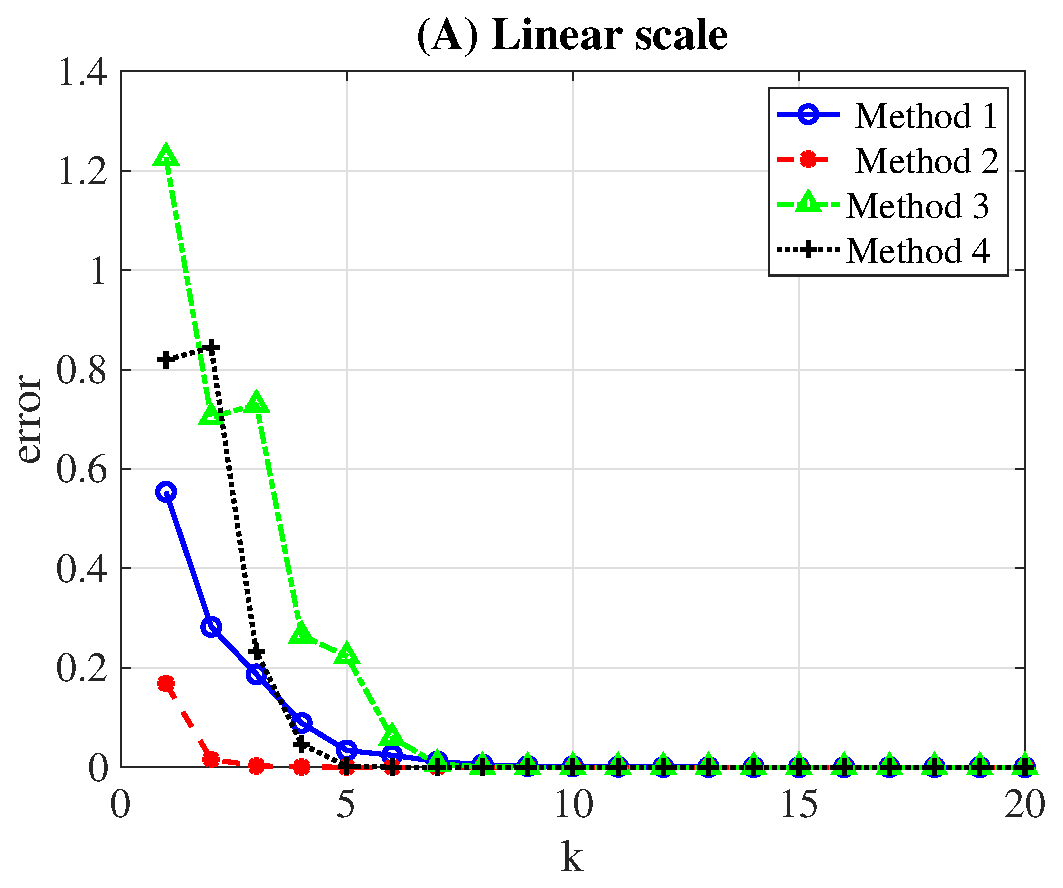
\includegraphics[width=0.3\textwidth]{figures/powerlaw2a}
      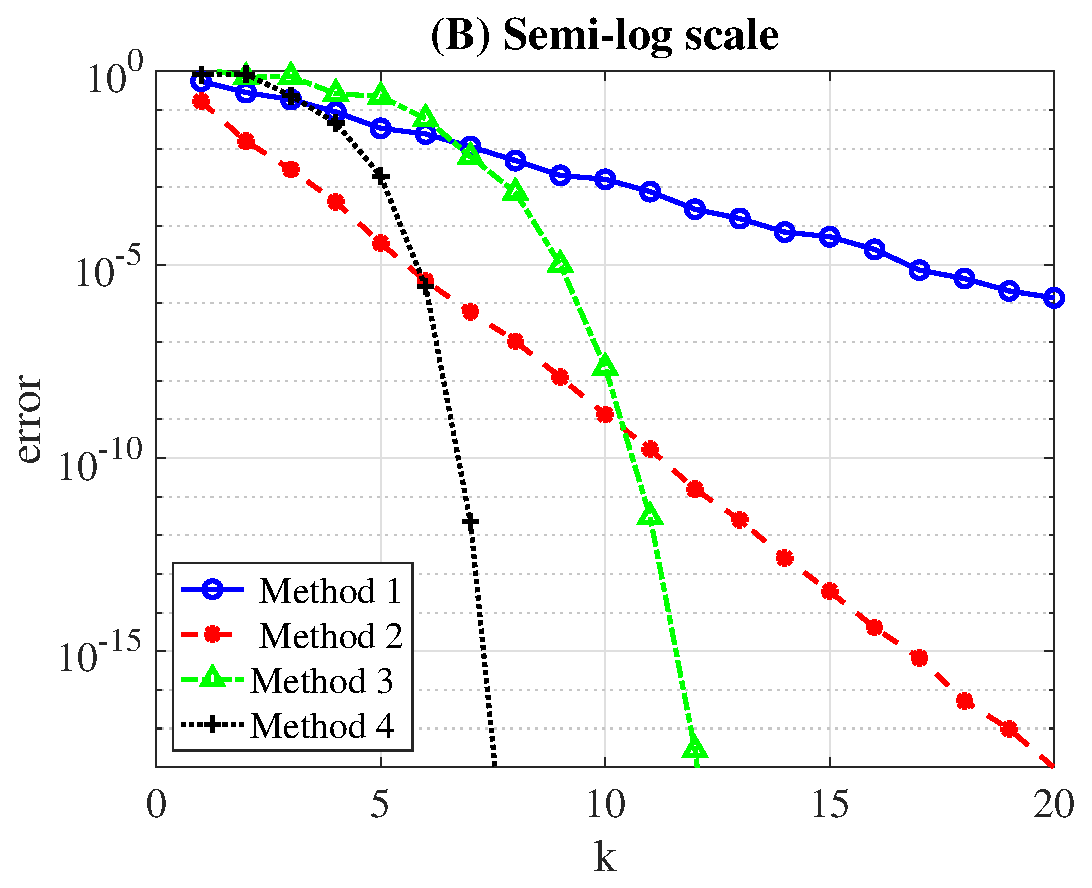
\includegraphics[width=0.3\textwidth]{figures/powerlaw2b}
      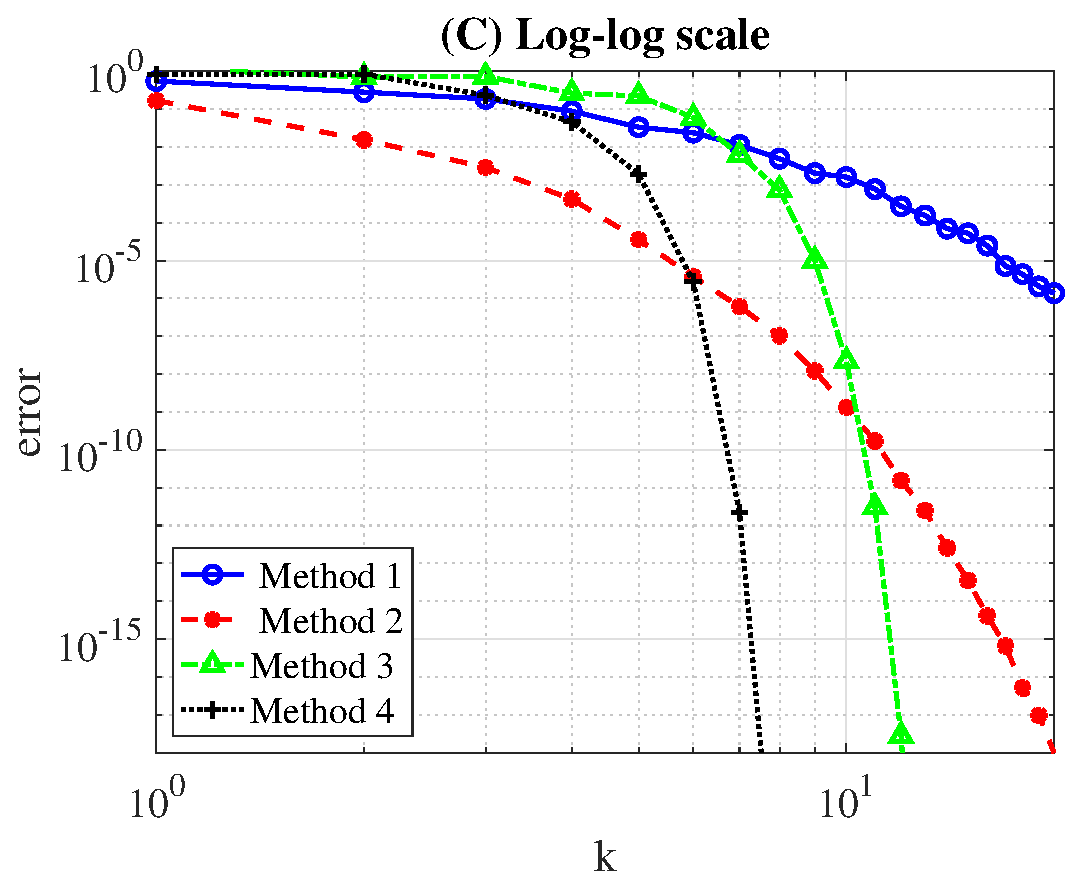
\includegraphics[width=0.3\textwidth]{figures/powerlaw2c}
    \end{center}}%
  {Linear scale}%
  {Semi-log scale}%
  {Log-log scale}%
  {2}{You want to choose an axis scaling where the behaviour of the
    method is represented as a straight line, since this linear dependence
    is easy to recognize visually.  The semi-log plot (B) is the only one
    that contains linear features (for Methods 1 \& 2).  We know that a
    linearly convergent method with $E_k \sim c E_0^k$ appears as a
    straight line on a semi-log scale.  So Methods 1 \& 2 are linearly
    convergent, while Methods 3 \& 4 are superlinear (faster than
    linear, but we can't say more than that.}{\jms}


\end{clicklist}

%%%%%%%%%%%%%%%%%%%%%%%%%%%%%%%%%%%%%%%%%%%%%%%%%%%%%%%%%%%%%%%%%%%%%%%%%%%%%%
\mysubhead{3d}{Iterative Methods for Sparse Systems}

\begin{clicklist}

  \qitemMCfour{Consider the $n\times n$ matrix
    \begin{gather*}
      A = \left[ 
        \begin{array}{cccccc}
          1 &  1 &  1 &  1 & \cdots & 1\\
          1 &  2 &  4 &  8 & \cdots & 2^{n-1}\\
          1 &  3 &  9 & 27 & \cdots & 3^{n-1}\\
          1 &  4 & 16 & 64 & \cdots & 4^{n-1}\\
          \vdots & \vdots & \vdots & \vdots & \ddots & \vdots \\
          1 &  n & n^2    & n^3  & \cdots & n^{n-1}
        \end{array}
      \right]
    \end{gather*}
    % Matrix det/cond/norm are calculated with 'matrix1.m'
    and suppose that for some given $n$ you know that
    % n=5:
    % $\operatorname{det}(A) = 288$, 
    % $\|A\|_1 = 979$ and
    % $\operatorname{cond}_1(A) = 44055$.
    % n=7: 
    $\operatorname{det}(A) = 2.49$e+07,\ %
    $\|A\|_1 = 1.85$e+05 and\ %
    $\operatorname{cond}_1(A) = 4.14$e+07.\ %
    Based on this information, which is the best method for solving the
    linear system $Ax=b$?}%
  {Gaussian elimination}%
  {Gaussian elimination with partial pivoting}%
  {Jacobi's iteration}%
  {Gauss-Seidel iteration}%
  {2}{This matrix is not sparse (far from it, since there's not a single
    zero entry!) and so iterative methods are a bad idea and Gaussian
    elimination is the only option.  The condition number is large,
    indicating that $A$ is ill-conditioned and partial pivoting is
    necessary.}{\jms}


  \qitemMCfour{Consider the $n\times n$ matrix
    \begin{gather*}
      A = \left[ 
        \begin{array}{rrrrrr}
          -4 &  1 &  0 & 0 & \cdots & 0\\
          1  & -4 &  1 & 0 & \cdots & 0\\
          0  &  1 & -4 & 1 & \cdots & 0\\
          \vdots& & \ddots & \ddots & \ddots & \vdots \\
          0  & \cdots & 0 & 1 & -4 &  1\\
          0  & \cdots & 0 & 0 &  1 & -4 
        \end{array}
      \right]
    \end{gather*}
    % Matrix det/cond/norm are calculated with 'matrix1.m'
    and suppose that for some given $n$ you know that 
    % n=5:
    % $\operatorname{det}(A) = -780$,  
    % $\|A\|_1 = 6$ and
    % $\operatorname{cond}_1(A) = 2.8846$.  
    % n=7: 
    $\operatorname{det}(A) = -10864$,\ %
    $\|A\|_1 = 6$ and\ %
    $\operatorname{cond}_1(A) = 2.97$.\ %
    Based on this information, identify the best method for solving the
    linear system $Ax=b$.}%
  {Gaussian elimination}%
  {Gaussian elimination with partial pivoting}%
  {Jacobi's iteration}%
  {Gauss-Seidel iteration}%
  {4}{This is a sparse system and so Gauss-Seidel is the ``obvious''
    answer.  However, we've seen in lectures that GE+PP can row-reduce
    this tridiagonal matrix with \myuline{no fill-in} and so it is a very
    efficient method -- so (B) is likely the best answer.}{}


  \qitemMCthree{If the $n\times n$ matrix $A$ is ill-conditioned (that
    is, $A$ has a very large condition number) then \dots}%
  {Solving $Ax = b$ accurately is difficult using the LU-decomposition, 
    but iterative methods (Jacobi, Gauss-Seidel) would not have a
    problem.}% 
  {Solving $Ax = b$ accurately with iterative methods (Jacobi,
    Gauss-Seidel) would be difficult, but LU-decomposition with partial
    pivoting would not have a problem.}% 
  {Solving $Ax = b$ accurately will be challenging regardless of the
    method we use.}%
  {3}{}{\jms}


  \qitemTF{You are given the $3 \times 3$ linear system in augmented
    matrix form
    \begin{gather*}
      \left[ \begin{array}{rrr:r}
        5 & 0 & -1 & 2 \\ 0 & 0 & 2 & 4 \\ 0 & 1 & 0 & 2
      \end{array} \right]
    \end{gather*}
    Because the diagonal of the coefficient matrix contains zero
    entries, it is not possible to apply the Jacobi iterative method.}%
  {FALSE}{Swapping rows 2 and 3 converts the matrix to upper triangular
    form with non-zeroes on the diagonal, and Jacobi can then be
    applied.}{\jms} 


  \qitemMCthree{You are given the $3 \times 3$ linear system in augmented
    matrix form
    \begin{gather*}
      \left[ \begin{array}{rrr:r}
        5 & 0 & -1 & 2 \\ 0 & 1 & 0 & 2 \\ 0 & 0 & 2 & 4 
      \end{array} \right]
    \end{gather*}
    Starting from an initial guess of $x_0 = [1, 1, 1]^T$, what is the
    result of the first iteration of the Jacobi method?}%
  {$x_1 = \left[\frac{3}{5}, 2, 2 \right]^T$}%
  {$x_1 = \left[\frac{2}{5}, 2, 1 \right]^T$}%
  {$x_1 = \left[\frac{3}{5}, 2, 5 \right]^T$}%
  {1}{\mbox{}\newline
    % \begin{gather*}      
    $\begin{array}{l} 
      x_1 = \frac{1}{5}\, (2-0\cdot 1 + 1\cdot 1) = \frac{3}{5}\\[0.2cm]
      x_2 = \frac{1}{1}\, (2-0\cdot 1 - 0\cdot 1) = 2\\[0.2cm]
      x_3 = \frac{1}{2}\, (4-0\cdot 1 - 0\cdot 1) = 2\\[0.3cm]
    \end{array}$\newline
    % \end{gather*}
    \underline{\smash{Interesting observation:}}~~Jacobi applied to
    \underline{\smash{any}} upper triangular $n\times n$ matrix
    converges to the exact solution in at most $n$ steps AND it's
    equivalent to doing backward substitution \dots\ although it can
    do a lot of extra work to get there!}{\jms}


  \qitemMCthree{You are given the $3 \times 3$ linear system in augmented
    matrix form
    \begin{gather*}
      \left[ \begin{array}{rrr:r}
        5 & 0 & -1 & 2 \\ 0 & 1 & 0 & 2 \\ 0 & 0 & 2 & 4 
      \end{array} \right]
    \end{gather*}
    Starting from an initial guess of $x_0 = [1, 1, 1]^T$, what is the
    result of the first iteration of the Gauss-Seidel method?}%
  {$x_1 = \left[\frac{3}{5}, 2, 2 \right]^T$}%
  {$x_1 = \left[\frac{2}{5}, 2, 1 \right]^T$}%
  {$x_1 = \left[\frac{3}{5}, 2, 5 \right]^T$}%
  {1}{This is identical to the Jacobi iteration because the lower
    triangular part of the matrix is 0!}{\jms}


  \qitemMCthree{You are given the $3 \times 3$ linear system in augmented
    matrix form
    \begin{gather*}
      \left[ \begin{array}{rrr:r}
        5 & 0 & -1 & 2 \\ 0 & 1 & 0 & 2 \\ 0 & -3 & 2 & 4 
      \end{array} \right]
    \end{gather*}
    Starting from an initial guess of $x_0 = [1, 1, 1]^T$, what is the
    result of the first iteration of the Gauss-Seidel method?}%
  {$x_1 = \left[\frac{3}{5}, 2, 2 \right]^T$}%
  {$x_1 = \left[\frac{2}{5}, 2, 1 \right]^T$}%
  {$x_1 = \left[\frac{3}{5}, 2, 5 \right]^T$}%
  {3}{\mbox{}\newline
    $\begin{array}{l} 
      x_1 = \frac{1}{5}\, (2-0\cdot 1 + 1\cdot 1) = \frac{3}{5}\\[0.2cm]
      x_2 = \frac{1}{1}\, (2-0\cdot\frac{3}{5} - 0\cdot 1) = 2\\[0.2cm]
      x_3 = \frac{1}{2}\, (4-0\cdot\frac{3}{5} + 3\cdot 2) = 5
    \end{array}$}{\jms}


  \qitemMCthree{You apply the Gauss-Seidel method to solve a linear
    system having an iteration matrix $T=-(D+L)^{-1}U$ with spectral
    radius $\rho(T)=0.998$.  Using the fact that $\log_{10}(0.998)
    \approx -0.0009$, roughly how many iterations are needed to reduce
    the error in the initial guess by a factor of $10^{-6}$?}%
  {6}%
  {600}%
  {6000}%
  {3}{The error estimate for a matrix iteration takes the form of an
    inequality for the error $E_k$ in step $k$: $E_k \leqslant \rho(T)^k
    E_0$.  If the error needs to reduce by a factor of $10^{-6}$ then
    \begin{gather*}
      \rho(T)^k \leqslant 10^{-6} \quad \Longrightarrow \quad 
      k \cdot \underbrace{\log_{10}(\rho(T))}_{-0.0009} \leqslant -6
      \quad \Longrightarrow \quad   
      k \geqslant \frac{-6}{-0.0009} \approx 6000
    \end{gather*}}{\jms}


  \qitemMCtwo{Below is the output from the Jacobi and Gauss-Seidel
    iterations for solving the linear system $Ax=b$, in each case
    showing the iteration number $k$ and the norm of the solution
    difference $\|x_k-x_{k-1}\|$:\\[0.3cm]
    \hspace*{0.05\textwidth}\begin{minipage}{0.4\textwidth}
      \ttfamily\underline{Method A:}\\
      k=~~~1:  6.073730e+00\\
      k=~~~2:  4.961063e+00\\
      k=~~~3:  4.408955e+00\\
      k=~~~4:  3.969368e+00\\
      k=~~~5:  3.620131e+00\\
      \mbox{}~~$\vdots$~~~~~~~~~~~$\vdots$\\
      k=~184:  1.366841e-06\\
      k=~185:  1.258350e-06\\
      k=~186:  1.158471e-06\\
      k=~187:  1.066519e-06\\
      k=~188:  9.818663e-07
    \end{minipage}
    \begin{minipage}{0.4\textwidth}
      \ttfamily\underline{Method B:}\\
      k=~~~1:  3.501795e+00\\
      k=~~~2:  2.710771e+00\\
      k=~~~3:  2.623906e+00\\
      k=~~~4:  2.353607e+00\\
      k=~~~5:  2.294563e+00\\
      \mbox{}~~$\vdots$~~~~~~~~~~~$\vdots$\\
      k=~354:  1.177728e-06\\
      k=~355:  1.130021e-06\\
      k=~356:  1.084248e-06\\
      k=~357:  1.040328e-06\\
      k=~358:  9.981874e-07
    \end{minipage}\\[0.3cm]
    Which method corresponds to the Jacobi iteration?}%
  {Method A}%
  {Method B}%
  {2}{Both converge, but Method A does so in about half the number of
    iterations.  This is characteristic of the Gauss-Seidel
    method.}{\jms} 

\end{clicklist}

%%%%%%%%%%%%%%%%%%%%%%%%%%%%%%%%%%%%%%%%%%%%%%%%%%%%%%%%%%%%%%%%%%%%%%%%%%%%%%
\mysubhead{3e}{Eigenvalue Problems}

[~nothing here yet~]

%%%%%%%%%%%%%%%%%%%%%%%%%%%%%%%%%%%%%%%%%%%%%%%%%%%%%%%%%%%%%%%%%%%%%%%%%%%%%%
\newpage
\myhead{4}{Function Approximation}

\mysubhead{4a}{Polynomial Interpolation}

\begin{clicklist}

  \qitemTF{Suppose that you have $n+1$ data points $(x_0, y_0)$, $(x_1,
    y_1)$, \dots, $(x_n, y_n)$. The interpolating polynomial on the
    given points is unique.}%
  {FALSE}{The $n^{\mathrm{th}}$ degree polynomial interpolating these
    points is unique, provided only that the $x_i$ are all
    distinct.}{Heath~\cite{heath-2018}, adapted from Review Question 7.3, p.~333}


  \qitemMCthree{Suppose that you have $n$ data points $(x_1, y_1)$,
    \dots, $(x_n, y_n)$, with the $x_i$ all distinct.  Which of the
    following statements about the $n^\mathrm{th}$ degree interpolating
    polynomial is TRUE?}%
  {The interpolating polynomial is unique.}%
  {There are infinitely many such interpolating polynomials.}%
  {There is no polynomial of this degree that interpolates all $n$
    points.}%
  {2}{An $n^{\mathrm{th}}$ degree polynomial has $n+1$ coefficients
    which are constrained by $n$ interpolating conditions. So there
    remains one degree of freedom.}{Heath~\cite{heath-2018}, adapted
    from Review Question 7.3, p.~333}
    

  \qitemMCfour{You determine a function $f(x)$ that passes through
    the points $(x_0,y_0)$, $(x_1,y_1)$, \dots, $(x_n, y_n)$ with $x_0 <
    x_1 < x_2 \cdots < x_n$. For some other point $x^*\in (x_0, x_n)$,
    you then use $f(x^*)$ to approximate the value of the actual smooth
    function that underlies the data.  This procedure is called:}%
  {interpolation}%
  {extrapolation}%
  {curve fitting}%
  {regression}%
  {1}{}{Holistic Numerical Methods~\cite{kaw-2019}}


  \qitemMCfour{\fillblank Suppose you have $n+1$ data points $(x_0,
    y_0)$, $(x_1, y_1)$, \dots, $(x_n, y_n)$. A unique polynomial of
    degree \myblank can be found that passes through these points.}%
  {$n$}%
  {$n$ or less}%
  {$n+1$}%
  {$n+1$ or more}%
  {2}{Assuming the $x_i$ are distinct, then there is a unique polynomial
    of degree exactly $n$ that passes through the $n+1$ data points.
    However, response (B) is the correct answer because if any of the
    $x_i$ are repeated, then some of the higher degree coefficients
    could be zero.}{Holistic Numerical Methods~\cite{kaw-2019}, MC
    Question\_Solution\ Ch\ 05.01\ Background\ of\ Interpolation.pdf}
  

  \qitemMCfour{How many different polynomials can be found that pass
    through the points $(1,2)$ and $(4,5)$? }%
  {1}%
  {2}%
  {1 or 2}%
  {infinitely many}%
  {4}{}{Holistic Numerical Methods~\cite{kaw-2019}, MC
    Question\_Solution Ch 05.01 Background of Interpolation.pdf}
  

  \qitemMCfour{You are given the point values $(1,1)$, $(2,4)$, $(3,9)$
    for some function $f(x)$.  You determine an approximation $P(x)$
    that passes through the 3 given points, and you then approximate 
    $f(4)$ using $P(4)$. What is this procedure called?}%
  {extrapolation}%
  {interpolation}%
  {curve fitting}%
  {none of the above}%
  {1}{Because $x=4$ lies outside the interval $[1,3]$ covered by the
    given $x$--coordinates.}{Holistic Numerical Methods~\cite{kaw-2019}}
  
  
  \qitemMCfourtwoc{The following data describes the velocity of a rocket
    during lift-off as a function of time:
    \begin{center}
      \begin{tabular}{c|cccccc}
        $t$ (s)      & 0 & 14 & 15 & 20 & 30 & 35 \\\hline
        $v(t)$ (m/s) & 0 & 227 & 363 & 517 & 603 & 902 
      \end{tabular}
    \end{center}
    In order to determine the velocity at $t=25\;s$, you decide to use a
    quadratic polynomial $v(t)=a + bt + ct^2$ to approximate the
    velocity profile.  The most appropriate system of equations for
    determining the coefficients is \dots}%
  {$\ds{\begin{bmatrix}
        1 & 14 & 176 \\ 1 & 15 & 225 \\ 1 & 20 & 400 
      \end{bmatrix}
      \begin{bmatrix}
        a \\ b \\ c 
      \end{bmatrix} = 
      \begin{bmatrix}
        227 \\ 363 \\ 517 
      \end{bmatrix}}$}%
  {$\ds{\begin{bmatrix}
        1 & 15 & 225\\ 1 & 20 & 400 \\ 1 & 30 & 900 
      \end{bmatrix}
      \begin{bmatrix}
        a \\ b \\ c 
      \end{bmatrix} = 
      \begin{bmatrix}
        363 \\ 517 \\ 603
      \end{bmatrix}}$}%
  {$\ds{\begin{bmatrix}
        1 & 0 & 0\\ 1 & 15 & 225 \\ 1 & 30 & 900 
      \end{bmatrix}
      \begin{bmatrix}
        a \\ b \\ c 
      \end{bmatrix} = 
      \begin{bmatrix}
        0 \\ 363 \\ 603
      \end{bmatrix}}$}%
  {$\ds{\begin{bmatrix}
        1 & 20 & 400\\ 1 & 30 & 900 \\ 1 & 35 & 1225
      \end{bmatrix}
      \begin{bmatrix}
        a \\ b \\ c 
      \end{bmatrix} = 
      \begin{bmatrix}
        517 \\ 603 \\ 902
      \end{bmatrix}}$}%
  {2}{Response (A) corresponds to extrapolation and (C) doesn't use the
  three data points closest to $t=25$, and so both will probably be less
  accurate.  Responses (B) and (D) should give comparable accuracy since
  they are based on intervals that are closest to the interpolation
  point.}{\jms} 


  \qitemMCfour{\fillblanks For the $n+1$ data points $(x_0, y_0)$,
    $(x_1, y_1)$, \dots, $(x_n,y_n)$, the $n^{\textrm{th}}$ degree
    Lagrange polynomial is $\ds{P_n(x) = \sum\limits_{j=0}^n y_j
      L_j(x)}$ where $\ds{L_j(x) = \prod\limits_{\substack{i=0\\ i\ne
          j}}^n \frac{(x-x_i)}{(x_j-x_i)}}$.

    To compute the computational cost, constructing each $L_j$ requires
    \mysmblank\circnum{1}\mysmblank multiplications and
    \mysmblank\circnum{2}\mysmblank divisions, and there are
    \mysmblank\circnum{3}\mysmblank such $L_j$ to compute. Evaluating
    the interpolating polynomial then requires a further $n+1$
    multiplications and $n$ additions. Therefore, assuming all
    operations involve the same work, the total cost is
    \mysmblank\circnum{4}\mysmblank $=O(n^2)$ operations.}%
  {\circnum{1}\ $n+1$, \circnum{2}\ $n+1$, \circnum{3}\ $n+1$,
    \circnum{4}\ $2(n+1)^2 + (2n+1)$}%
  {\circnum{1}\ $n$,~~~~~ \circnum{2}\ $n$,~~~~~~ \circnum{3}\ $n$,~~~~~
    \circnum{4}\ $2n(n+1)(2n+1)$}%
  {\circnum{1}\ $n$,~~~~~ \circnum{2}\ $n$,~~~~~~ \circnum{3}\ $n$,~~~~~
    \circnum{4}\ $2n^2 + (2n+1)$}%
  {\circnum{1}\ $n$,~~~~~ \circnum{2}\ $n$,~~~~~~ \circnum{3}\ $n+1$,
    \circnum{4}\ $2n(n + 1) + (2n+1)$}%
  {4}{}{\jms, \courseID lecture notes}
  
  
  \qitemMCfour{%
    \mytwocol[0.6]{For the $n+1$ data points $(x_0, y_0), (x_1, y_1),
      \dots, (x_n, y_n)$, the $n^{\textrm{th}}$ degree Lagrange
      polynomial is $\ds{P_n(x) = \sum\limits_{j=0}^ny_jL_j(x)}$ where
      $\ds{L_j(x) = \prod\limits_{\substack{i=0 \\ i\ne j}}^n
        \frac{(x-x_i)}{(x_j-x_i)}}$.
      
      The given partial code calculates a single Lagrange polynomial
      $L_j$, where the given $x$-coordinates are assigned to the
      variable {\tt xdata}. Provide suitable code to fill the blank
      spaces labelled \circnum{1}\ and \circnum{2}.}%
    {{\tt
        Lj = ...\circnum{1}...\\
        for i = 1:n,
        
        ~~~if i $\sim$= j,
        
        ~~~~~~Lj = ...\circnum{2}... 
        
        ~~~end\\        
        end}}}%
  {{\tt ~~\circnum{1}~0.0; ~~~\circnum{2}~Lj*(x-xdata(i))/(xdata(j)-xdata(i));}}%
  {{\tt ~~\circnum{1}~1.0; ~~~\circnum{2}~Lj*(x-xdata(i))/(xdata(j)-xdata(i));}}%
  {{\tt ~~\circnum{1}~1.0; ~~~\circnum{2}~(x-xdata(i))/(xdata(j)-xdata(i));}}%
  {{\tt ~~\circnum{1}~0.0; ~~~\circnum{2}~(x-xdata(i))/(xdata(j)-xdata(i));}}%
  {2}{}{\jms, \courseID lecture notes}
  
  
  \qitemMCfour{The linear Lagrange polynomial that interpolates
    the points ($x_1, f(x_1)$) and ($x_2, f(x_2)$) is}%
  {$\ds{P(x) = \frac{(x-x_2)}{(x_1-x_2)}f(x_1) + \frac{(x-x_1)}{(x_2-x_1)}f(x_2)}$}%
  {$\ds{P(x) = \frac{(x_1-x_2)}{(x-x_2)}f(x_1) + \frac{(x_2-x_1)}{(x-x_1)}f(x_2)}$}%
  {$\ds{P(x) = \frac{f(x_1)-f(x_2)}{(x_1-x_2)} x + \frac{x_1 f(x_2) - x_2 f(x_1)}{(x_1-x_2)}}$}%
  {$\ds{P(x) = \frac{x}{(x_1-x_2)}f(x_1) + \frac{x}{(x_2-x_1)}f(x_2)}$}%
  {1}{}{} 
  
  
  \qitemMCfour{This table lists the population of Canada every 5
    years from 2000 to 2015: 
    \begin{center}
      \begin{tabular}{c|c|c|c|c}%\hline
        Year & 2000 & 2005 & 2010 & 2015 \\\hline
        Population (in millions) & 30.69 & 32.24 & 34.01 & 35.83
        %\hline
      \end{tabular}
    \end{center}
    Using the Lagrange interpolating polynomial to express the
    population as
    \begin{gather*}
      P(x) = 30.69\, L_0(x) + 32.24\, L_1(x) + 34.01\, L_2(x) + 35.83\,
      L_3(x), 
    \end{gather*}
    one can approximate the population in any year $x$ between 2000 to
    2015.  What is $L_0(x)$?}%
  {$\ds{\frac{(x-2005)(x-2010)(x-2015)}{750}}$}%
  {$\ds{\frac{(x-2005)(x-2010)(x-2015)}{-750}}$}%
  {$\ds{\frac{(x-2000)(x-2005)(x-2010)}{-50}}$}%
  {$\ds{\frac{(x-2000)(x-2010)(x-2015)}{-150}}$}%
  {2}{This is the only polynomial that satisfies $L_0=1$ at $x=2000$ and
    $L_0=0$ at the other three data points.}{\mah}


  \qitemMCfour{Fill in the blanks in the divided difference table:
    \begin{center}
      \begin{tabular}{c|ccc}
        $x$& $y$& & \\ 
        \hline
        1 & 1 &             & \\[-3pt]
        ~ &   & \circnum{a} & \\[-3pt]
        3 & 9 &             & \circnum{c} \\[-3pt]
        ~ &   & \circnum{b} & \\[-3pt]
        4 & 16&             &
      \end{tabular}
    \end{center}}%
  {$\circnum{a} = 4$, \quad $\circnum{b} = 7$, \quad $\circnum{c} = 1$}%
  {$\circnum{a} = 8$, \quad $\circnum{b} = 7$, \quad $\circnum{c} = 3$}%
  {$\circnum{a} = 8$, \quad $\circnum{b} = 4$, \quad $\circnum{c} = 3$}%
  {$\circnum{a} = 7$, \quad $\circnum{b} = 4$, \quad $\circnum{c} = 3$}%
  {1}{Following the Newton divided difference formula, we have 
    \begin{gather*}
      \circnum{a} = \frac{9-1}{3-1}  = 4, \quad 
      \circnum{b} = \frac{16-9}{4-3} = 7 \quad \text{and then} \quad 
      \circnum{c} = \frac{7-4}{4-1}  = 1.
    \end{gather*}}{\mah}
  

  \qitemMCfour{%
    \mytwocol[0.55]{The second degree polynomial
      \begin{gather*}
        P_2(x) = a_1 + a_2 (x-3) + a_3 (x-3)(x-4)
      \end{gather*}
      is determined using the given table of Newton divided differences.
      The correct value of $a_2$ is \dots}%
    {\begin{tabular}{c|cccc}
        $x$ & $y$ &   &   &  \\\hline
        1   & 1   &   &   &  \\[-3pt]
        ~   &     & 4 &   &  \\[-3pt]
        3   & 9   &   & 1 &  \\[-3pt]
        ~   &     & 7 &   & 0\\[-3pt]
        4   & 16  &   & 1 &  \\[-3pt]
        ~   &     & 9 &   &  \\[-3pt]
        5   & 25  &   &   &  
      \end{tabular}}}%
  {$a_2 = 1$}%
  {$a_2 = 4$}%
  {$a_2 = 7$}%
  {$a_2 = 9$}%
  {3}{It's the second diagonal in the table that starts at the point
    $x=3$, for which the interpolating polynomial is:
    \begin{gather*}
      P_2(x) = 9 + 7 (x-3) + 1 (x-3)(x-4).
    \end{gather*}}{Holistic Numerical Methods~\cite{kaw-2019}}
  
  
  \qitemMCfour{%
    \mytwocol[0.55]{The second degree polynomial
      \begin{gather*}
        P_2(x) = 4 + 6 (x-a) + (x-b)(x-c).
      \end{gather*}
      is determined using the given table of Newton divided differences.
      The correct values of the coefficients are \dots}%
    {\begin{tabular}{c|cccc}
        $x$ & $y$ &   &   &  \\\hline
        1   & 1   &   &   &  \\[-3pt]
        ~   &     & 3 &   &  \\[-3pt]
        2   & 4   &   & 1 &  \\[-3pt]
        ~   &     & 6 &   & 0\\[-3pt]
        4   & 16  &   & 1 &  \\[-3pt]
        ~   &     & 9 &   &  \\[-3pt]
        5   & 25  &   &   &  
      \end{tabular}}}%
  {$a = 1$, \quad $b=2$, \quad $c=4$}%
  {$a = 2$, \quad $b=2$, \quad $c=4$}%
  {$a = 1$, \quad $b=3$, \quad $c=1$}%
  {$a = 2$, \quad $b=4$, \quad $c=5$}%
  {2}{These coefficients come from the second diagonal in the table,
    which starts at the point $x=2$, so the interpolating polynomial is
    \begin{gather*}
      P_2(x) = 4 + 6 (x-2) + (x-2)(x-4).
    \end{gather*}}{\mah}               
  
  
  \qitemMCfour{%
    \mytwocol[0.55]{Which of the following is a third degree
      interpolating polynomial for the data given in the Newton divided
      difference table.}%
    {\begin{tabular}{c|ccccc}
        $x_i$ & $a_0$ & $a_1$ & $a_2$ & $a_3$ & $a_4$ \\\hline 
        0     & 0     &       &       &       &   \\[-3pt]
        ~     &       &  1    &       &       &   \\[-3pt]
        1     & 1     &       & 3     &       &   \\[-3pt]
        ~     &       &  7    &       & 1     &   \\[-3pt]
        2     & 8     &       & 6     &       & 0 \\[-3pt]
        ~     &       &  19   &       & 1     &   \\[-3pt]
        3     & 27    &       & 9     &       &   \\[-3pt]
        ~     &       &  37   &       &       &   \\[-3pt]
        4     &  64   &       &       &       &   
      \end{tabular}}}%
  {$P_3(x) = x + 3x(x-1) + x(x-1)(x-2)$}%
  {$P_3(x) = 1+ 7(x-1) + 6(x-1)(x-2) + (x-1)(x-2)(x-3)$}%
  {$P_3(x) = 64+ 37(x-4) + 9(x-4)(x-3) + (x-4)(x-3)(x-2)$}%
  {All of the above}%
  {4}{}{\mah}
  
  
  \qitemMCfour{Consider the interpolating polynomial for $f(x) = x^3$
    based on the points $(1,1)$, $(2,8)$, $(3,27)$, and $(4,64)$. Find
    an upper bound for the interpolation error on $[1,4]$.}%
  {$\frac{1}{6}$}%
  {$\frac{15}{8}$}%
  {$\frac{105}{16}$}%
  {0}%
  {4}{There are four points so the interpolating polynomial is a cubic.
    Since the original function is a cubic, then $P_3(x)=x^3$, so the
    error is zero!  You could also use the error formula
    \begin{gather*} 
      |f(x) - P_3(x)| \leqslant \left| \frac{f^{(4)}(c)}{4!}
        (x-1)(x-2)(x-3)(x-4) \right| = 0
    \end{gather*}
    because $f^{(4)}(x)\equiv 0$.}{\mah}
  
  
  \qitemMCfour{Consider the interpolating polynomial for $f(x) = x^3$
    based on the points $(0,0)$, $(1,1)$ and $(2,8)$.  Find an upper bound for
    the interpolation error at the point $x=\half$.}%
  {$\frac{1}{6}$}%
  {$1$}%
  {$\frac{15}{8}$}%
  {$\frac{3}{8}$}%
  {4}{Since there are three points, the interpolating polynomial is a
    quadratic for which the error formula gives
    \begin{align*}
      |f(x) - P_2(x)| &\leqslant \left| \frac{f'''(c)}{3!} \, x(x-1)(x-2)
      \right|\\[5pt]
      \implies {\textstyle \left| f(\half) - P_2(\half) \right|} 
      &\leqslant {\textstyle \left| \frac{6}{6}\, 
          \left(\half\right) \left(\half-1\right) \left(\half-2\right)
        \right| = \frac{3}{8}}.
    \end{align*}}{\mah}

  
  \qitemMCfour{%
    \mytwocol[0.55]{How many fourth-degree polynomials pass through the
      points $(1,1)$, $(2,8)$, $(3,27)$ and $(4,64)$? \\

      Hint: You might be able to use the Newton divided difference table
      to help you decide.}%
    {\begin{tabular}{c|cccccc}
        $x$ & $y$ &    &   &   \\\hline
        1   & 1   &    &   &   \\[-3pt]
        ~   &     & 7  &   &   \\[-3pt]
        2   & 8   &    & 6 &   \\[-3pt]
        ~   &     & 19 &   & 1 \\[-3pt]
        3   & 27  &    & 9 &   \\[-3pt]
        ~   &     & 37 &   &   \\[-3pt]
        4   & 64  &    &   &   
        %~  &     & *  &   &   & \\[-3pt]
        %a  & b   &    &   &   &  
      \end{tabular}}}%
  {1}%
  {2}%
  {none}%
  {infinitely many}%
  {4}{From the table, it's easy to determine a cubic polynomial that
    interpolates the four points:
    \begin{gather*}
      P_3(x) = 1 + 7(x-1) + 6(x-1)(x-2) + 1(x-1)(x-2)(x-3)
    \end{gather*}
    Then, we can generate a fourth-degree polynomial by adding any other
    point $(a,b)$ which will generate an extra coefficient $c$ in the
    table.  This corresponds to a new polynomial
    \begin{gather*}
      P_4(x) = P_3(x) + c(x-1)(x-2)(x-3)(x-4)
    \end{gather*}
    that interpolates the original four points, plus $(a,b)$.}{\mah} 
  
  
  \qitemMCfour{%
    \mytwocol[0.55]{How many third-degree polynomials pass through the
      points $(1,1)$, $(2,8)$, $(3,27)$ and $(4,64)$?\\
      
      Hint: You might be able to use the Newton divided difference table
      to help you decide.}%
    {\begin{tabular}{c|cccc} $x$ & $y$ & & & \\\hline
        1   & 1   &    &   &  \\[-3pt]
        ~   &     & 7  &   &  \\[-3pt]
        2   & 8   &    & 6 &  \\[-3pt]
        ~   &     & 19 &   & 1\\[-3pt]
        3   & 27  &    & 9 &  \\[-3pt]
        ~   &     & 37 &   &  \\[-3pt]
        4 & 64 & & &
      \end{tabular}}}%
  {1}%
  {2}%
  {3}%
  {infinitely many}%
  {1}{The divided difference table gives us a unique third-degree polynomial
    that can be written in two ways
    \begin{align*}
      P_3(x) &= 1 + 7(x-1) + 6(x-1)(x-2) + 1(x-1)(x-2)(x-3) \\
      &= 64 + 37(x-4) + 9(x-4)(x-3) + 1(x-4)(x-3)(x-2)
    \end{align*}
    (expand them both to show they're the same polynomial).}{\mah}
  
  
  \leavethisout{
    \qitemMCfour{How many first or second degree polynomials pass through
      the points $(1,1)$, $(2,8)$, $(3,27)$, and $(4,64)$?
      \begin{center}
        \begin{tabular}{c|cccc}
          $x$ & $y$ & &  &   \\
          \hline
          1 & 1  &    &    &   \\
          ~ &    & 7  &    &   \\
          2 & 8  &    & 6 &   \\
          ~ &    & 19 &   & 1 \\
          3 & 27 &    & 9 &   \\
          ~ &    & 37 &    &   \\
          4 & 64 &    &    &   \\
        \end{tabular}
      \end{center}}%
    {2}%
    {4}%
    {none}%
    {infinitely many}%
    {3}{There are no interpolating polynomials of degree 1 or 2.}{\mah}              
  }
    

  \qitemMCfour{Fill in the blanks in the divided difference table:
    \begin{center}
      \begin{tabular}{c|ccc}
        $x$ & $y$       &           &    \\\hline
        1   & 1         &           &    \\[-3pt]
        ~   &           &\circnum{b}&    \\[-3pt]
        2   &\circnum{a}&           & -1 \\[-3pt]
        ~   &           & 4         &    \\[-3pt]
        4   & 16        &           & 
      \end{tabular}
    \end{center}}%
  {$\circnum{a} = 8$, \quad $\circnum{b} = 7$}%
  {$\circnum{a} = 7$, \quad $\circnum{b} = -\frac{3}{4}$}%
  {$\circnum{a} = 8$, \quad $\circnum{b} = -3$}%
  {$\circnum{a} = 8$, \quad $\circnum{b} = -\frac{3}{2}$}%
  {1}{%Following the divided difference formula we have 
    %\begin{gather*}
    %  \frac{4 - \beta}{4 - 1} = -1 \Rightarrow \beta = 7.
    %\end{gather*}
    %and also 
    %\begin{gather*}
    %  \frac{16 - \alpha}{4 - 2} = 4 \Rightarrow \alpha = 8.
    %\end{gather*}
  }{\mah}

\end{clicklist}

%%%%%%%%%%%%%%%%%%%%%%%%%%%%%%%%%%%%%%%%%%%%%%%%%%%%%%%%%%%%%%%%%%%%%%%%%%%%%%
\mysubhead{4b}{Piecewise Polynomial or Spline Interpolation}

\begin{clicklist}

  \qitemMCfour{Which of the following is NOT a valid reason for choosing
    piecewise cubic over piecewise linear interpolation?}%
  {Piecewise cubics can yield an interpolating function that has
    continuous derivatives.}% 
  {Piecewise cubics generally converge to the underlying function faster
    than linear interpolants when the number of data points is
    increased.}%
  {Piecewise cubics are cheaper to compute.}%
  {Piecewise cubics can predict derivative values better than linear
    interpolants.}%
  {3}{Linear splines are built from polynomials of degree 1, which
    require many fewer operations to construct and evaluate than 
    cubic splines built with degree 3 polynomials.}{\jms} 


  \qitemTF{This piecewise polynomial is a quadratic spline:
    \begin{gather*}
      S(x) = \begin{cases}
          0,   & \text{if } -1\leqslant x \leqslant 0 \\
          x^2, & \text{if } 0 \leqslant x \leqslant 1
        \end{cases} 
    \end{gather*}}%
  {TRUE}{The piecewise functions are both quadratic, and $S(x)$ and
    $S'(x)$ match at $x=0$.}{\mah}
  

  \qitemMCfour{This piecewise polynomial is NOT a cubic spline:
    \begin{gather*}
      S(x) = \begin{cases}
        S_0(x) = 1,           & \text{if } 0\leqslant x\leqslant 1 \\
        S_1(x) = 1 + (x-1)^2, & \text{if } 1\leqslant x\leqslant 2
        \end{cases}
    \end{gather*}
    Why not?}%  
  {$S_0(1) \ne S_1(1)$}%
  {$S_0'(1) \ne S_1'(1)$}%
  {$S_0''(1) \ne S_1''(1)$}%
  {$S_0'''(1) \ne S_1'''(1)$}%
  {3}{}{\mah}

  
  \qitemTF{This piecewise polynomial cannot be a cubic spline: 
    \begin{gather*}
      S(x) = \begin{cases}
        S_0(x) = 1 + x + x^2 + x^3,             & \text{if } 0\leqslant x\leqslant 1 \\
        S_1(x) = 4 + (x-1) + (x-1)^2 + (x-1)^3, & \text{if } 1\leqslant x\leqslant 2
      \end{cases} 
    \end{gather*}}%
  {TRUE}{Although $S_0(1)=S_1(1)=4$, the derivatives don't match at
    $x=1$.}{\mah} 


  \qitemMCfour{In cubic spline interpolation, which spline derivatives
    must be continuous at interior points?}%
  {first derivatives}%
  {second derivatives}%
  {first and second derivatives}%
  {third derivatives}%
  {3}{}{Holistic Numerical Methods~\cite{kaw-2019}}


  \qitemMCfour{Suppose that 
    \begin{gather*}
      S(x) = \begin{cases}
        S_0(x) = 1 + a x + x^2 - x^3,              
        & \text{if } 0\leqslant x\leqslant 1 \\
        S_1(x) = 1 + b (x-1) - 2(x-1)^2 + (x-1)^3, 
        & \text{if } 1\leqslant x\leqslant 2
      \end{cases}
    \end{gather*}
    is a clamped cubic spline.  What are the clamped end-point slopes?}%
  {$S'(0)=0$ and $S'(2)=-1$}%
  {$S'(0)=1$ and $S'(2)=-2$}%
  {$S'(0)=0$ and $S'(2)=-2$}%
  {none of the above}%
  {3}{The matching conditions at $x=1$ require that 
    \begin{gather*}
      S_0(1) = S_1(1) \quad \Longrightarrow \quad 1+a+1-1 = 1 
      \quad \Longrightarrow \quad a=0\\
      S^\prime_0(1) = S^\prime_1(1) \quad \Longrightarrow \quad a+2-3 = b
      \quad \Longrightarrow \quad b=-1
    \end{gather*}
    Then $S_0'(0)=a=0$ and $S_1'(2)=b-1=-2$.}{\mah}
  

  \qitemMCfour{A cubic spline is defined as
    \begin{gather*}
      S(x) = \begin{cases}
        S_0(x) = 1 + c x^2 + x^3,                     
        & \text{if } 0\leqslant x\leqslant 1 \\
        S_1(x) = 2 + 3 (x-1) + 3 (x-1)^2 + d (x-1)^3, 
        & \text{if } 1\leqslant x\leqslant 2
      \end{cases}
    \end{gather*}
    Assuming that natural end-point conditions are used, determine the
    constants $c$ and $d$.}%
  {$c = 0$ and $d = -1$}%
  {$c = 0$ and $d = 1$}%
  {$c = 1$ and $d = 1$}%
  {$c = 1$ and $d = -1$}%
  {1}{Differentiate to get $S_0''=2c+6x$ and $S_1''=6+6d(x-1)$.  Then
    the natural end-point conditions $S_0''(0)=2c=0$ and
    $S_1''(2)=6+6d=0$ are easy to solve.}{\mah}


  \qitemMCfour{A cubic spline is defined by
    \begin{gather*}
      S(x) = \begin{cases}
          S_0(x) = 1 + bx + cx^2 - 2x^3,              
          & \text{if } 0\leqslant x\leqslant 1 \\
          S_1(x) = 2 - 3(x-1)^2 + 2(x-1)^3, 
          & \text{if } 1\leqslant x\leqslant 2
        \end{cases} 
    \end{gather*}
    Assuming that periodic end-point conditions are used,
    determine the constants $b$ and $c$.}% 
  {$b = 0$ and $c = 3$}%
  {$b = 3$ and $c = 0$}%
  {$b = 1$ and $c = 3$}%
  {$b = 0$ and $c = 1$}%
  {1}{}{\mah}


  \qitemMCfour{A cubic spline is defined by 
    \begin{gather*}
      S(x) = \begin{cases}
        S_0(x) = a_0 + b_0 x + c_0 x^2 + d_0 x^3,             
        & \text{if } 0\leqslant x\leqslant 1 \\
        S_1(x) = a_1 + b_1 (x-1) + c_1 (x-1)^2 + d_1 (x-1)^3, 
        & \text{if } 1\leqslant x\leqslant 2 \\
        S_2(x) = a_2 + b_2 (x-2) + c_2 (x-2)^2 + d_2 (x-2)^3, 
        & \text{if } 2\leqslant x\leqslant 3 
      \end{cases}
    \end{gather*}
    Assuming that not-a-knot end-point conditions are used,
    which of the following statements about the coefficients is TRUE?}%
  {$a_0 = a_1 = a_2$}%
  {$b_0 = b_1 = b_2$}%
  {$c_0 = c_1 = c_2$}%
  {$d_0 = d_1 = d_2$}%
  {4}{The not-a-knot end-point conditions match $S_0'''(1)=S_1'''(1)$ and
    $S_1'''(2)=S_2'''(2)$.  Using $S_0'''=6d_0$, $S_1'''=6d_1$ and
    $S_2'''=6d_2$, it's easy to see that $d_0=d_1=d_2$.}{\mah}
  

  \qitemMCthree{%
    \mytwocol{The data shown in the plot is interpolated with three
      splines using different end-point conditions: natural, not-a-knot
      and clamped (zero slopes).  Identify the spline corresponding to
      each choice of end-point condition.}%
    {% Matlab code: splinecompare.m
      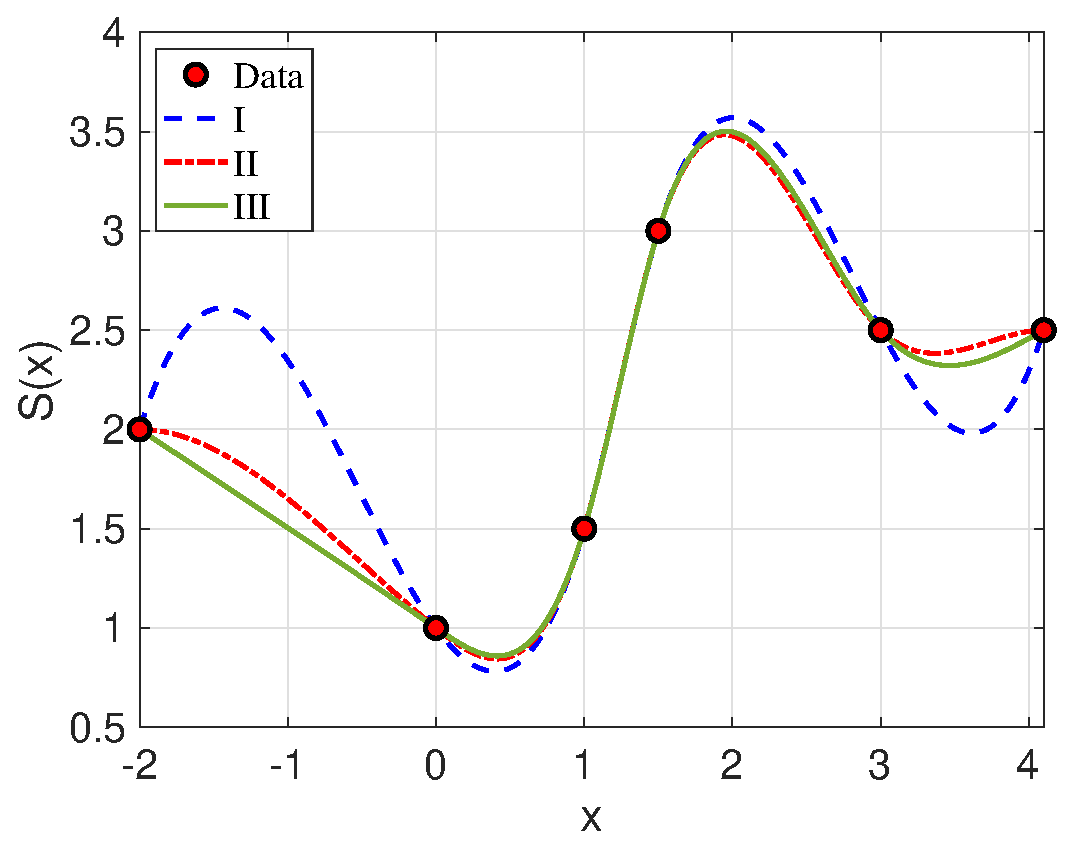
\includegraphics[width=\textwidth]{figures/splinecompare}}}%
  {I $=$ not-a-knot, ~~ II $=$ clamped,    ~~ III $=$ natural}%
  {I $=$ natural,    ~~ II $=$ not-a-knot, ~~ III $=$ clamped}%
  {I $=$ natural,    ~~ II $=$ clamped,    ~~ III $=$ not-a-knot}%
  {1}{Spline III has the smallest curvature near end-points, so this must
    be the natural spline.  Spline II is the only one with zero slope at
    both ends, so this is the clamped spline.}{\jms}


  \qitemTF{Suppose you have $n+1$ data points and interpolate them using 
    splines with degree $n$ (that is, $n+1$ piecewise polynomials each
    having degree $n$).  The resulting splines are all identical and
    equal to the interpolating polynomial that you would have obtained
    using a method like Lagrange interpolation.}%
  {TRUE}{}{\jms}

\end{clicklist}

%%%%%%%%%%%%%%%%%%%%%%%%%%%%%%%%%%%%%%%%%%%%%%%%%%%%%%%%%%%%%%%%%%%%%%%%%%%%%%
\mysubhead{4c}{Least Squares Fitting or Regression}

\begin{clicklist}
  
  \qitemMCfour{For each plot, identify the type of approximation that
    has been performed:\\ 
    \begin{minipage}[t]{0.45\textwidth}
      \vspace{0pt}
      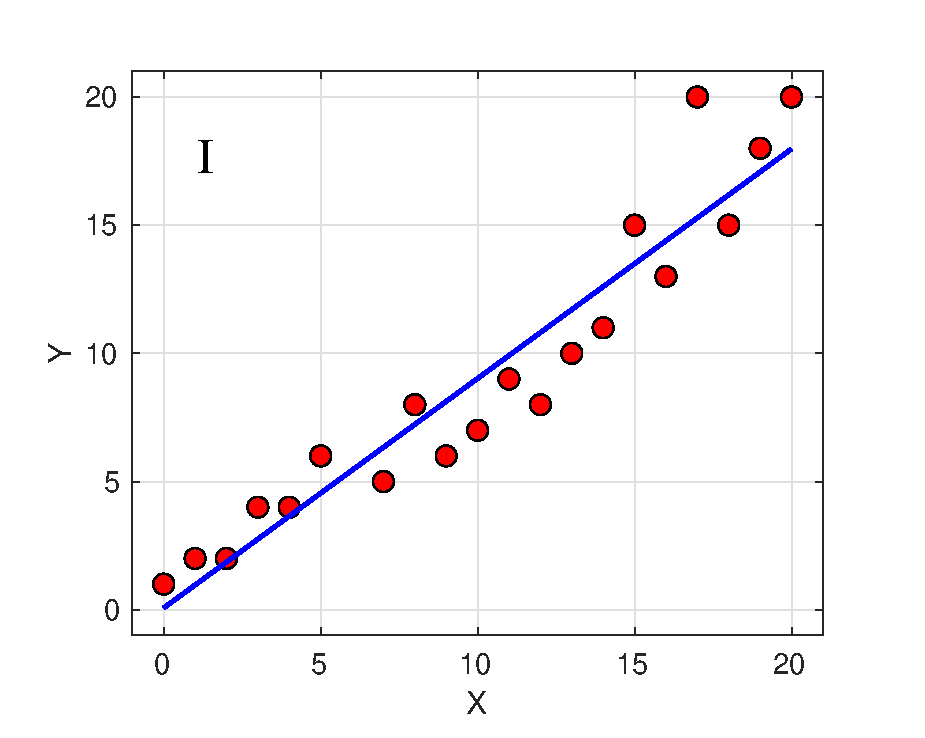
\includegraphics[width=0.9\textwidth]{figures/lsf_fit}
    \end{minipage}
    \quad
    \begin{minipage}[t]{0.45\textwidth}
      \vspace{0pt}
      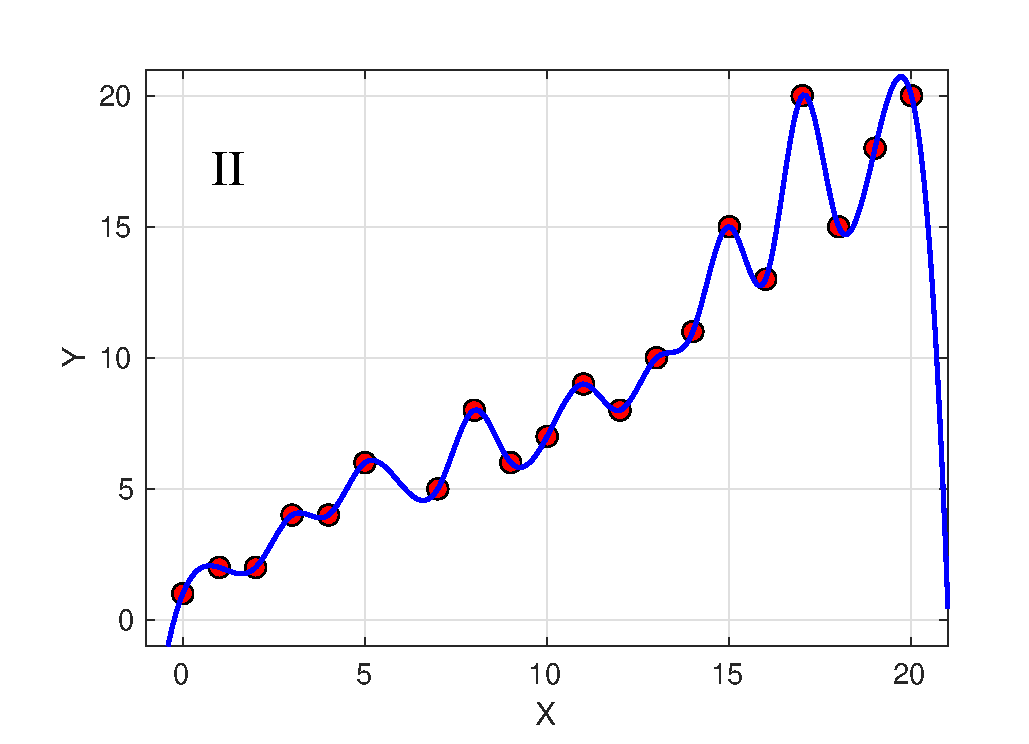
\includegraphics[width=\textwidth]{figures/lsf_interpolation}
    \end{minipage}}%
  {I $=$ interpolation, \quad II $=$ curve fitting}%
  {I $=$ curve fitting, \quad II $=$ interpolation}%
  {I $=$ interpolation, \quad II $=$ extrapolation}%
  {I $=$ extrapolation, \quad II $=$ interpolation}%
  {2}{}{\mah}


  \qitemMCfour{You are writing a \Matlab code that computes a
    least-squares fit {\tt yfit} to a set of data values {\tt ydata},
    both of which are vectors of length {\tt m}.  Which of the following
    lines of code computes the root mean square (RMS) error for the
    fit?%
    % The standard measure of fitting error is called root mean
    % square (RMS) error:
    % \begin{gather*}
    %   RMS = \sqrt{\frac{1}{m+1}\sum\limits_{i=0}^m(y_i - P(x_i))^2}
    % \end{gather*}
    % \Matlab vector {\tt yfit} represents $P(x_i)$ for all $x_i$. What
    % will be the \Matlab code for finding RMS?
  }%
  {{\tt RMS = sqrt(m * sum((yfit-y).\textasciicircum{}2));}}%
  {{\tt RMS = sqrt(sum((yfit-y).\textasciicircum{}2)) / m;}}%
  {{\tt RMS = sqrt(sum(yfit-y).\textasciicircum{}2 / m);}}%
  {{\tt RMS = sqrt(sum((yfit-y).\textasciicircum{}2) / m);}}%
  {4}{}{\jms, \courseID lecture notes}
  
    
  \qitemMCfour{%
    \mytwocol{The plot depicts noisy data points that were measured in
      an experiment.  What is the best choice of method for computing a
      smooth function that best approximates such noisy data?}%
    {% Matlab code: interpnoisy.m
      \includegraphics[width=\textwidth]{figures/interpnoisy1saveB}}}%
  {A single polynomial interpolant, because it represents the data
    exactly.}%
  {A piecewise cubic spline, because the resulting curve will be smooth
    at each data point.}%
  {A least-squares fit, because it can capture the overall trends in the
    data.}%
  {None will work because this data is too noisy.}%
  {3}{The data follow a trend that seems close to a cubic, but it's a
    bit noisy which suggests that neither interpolation method (A,B)
    will work very well.  The plot below demonstrates clearly how the
    polynomial and spline interpolants can be extremely ``wiggly'' even
    in the presence of small amounts of noise.  On the other hand, the
    least-squares cubic fit is smooth and also matches the data pretty
    closely.  In fact, if it weren't for the two points closest to
    $x=0$, both interpolants would be much closer to the cubic fit!!
    \begin{center}      
      % Matlab code: interpnoisy.m
      \includegraphics[width=0.4\textwidth]{figures/interpnoisy2saveB}
    \end{center}}{\jms}

  
  \qitemTF{Given $n$ data points $(x_i, y_i)$ with all of the $x_i$
    distinct, you apply the method of least squares to fit a $p^{th}$
    degree polynomial to the given data.  If $p=n-1$ then this is
    equivalent to polynomial interpolation.}%
  {TRUE}{When $p=n-1$, the least squares matrix is size $n\times n$
    and has the same structure as the Vandermonde matrix.}{\jms}
    

  \qitemTF{When fitting a straight line $y=a_0 + a_1 x$ to the three
    data points $(x_i, y_i) = (0,0)$, $(1,0)$ and $(1,1)$, the least
    squares solution is unique.}%
  {TRUE}{The method of least squares has no difficulty with the fact
    that the last two points have the same $x$-coordinate.  In this
    case, the linear fit bisects the repeated points as shown in the
    plot. 
    \begin{center}
      % Matlab code: lsqex1.m
      \includegraphics[width=0.4\textwidth]{figures/lsqex1}
    \end{center}}{Heath~\cite{heath-2018}, Exercise 3.4, p.~148}


  \qitemMCfour{%
    \mytwocol{Over the last century trade has grown remarkably. The
      graph shows the value of the world export index over the period
      1900--2000 along with a least squares fit. What type of fit is
      it?}%
    {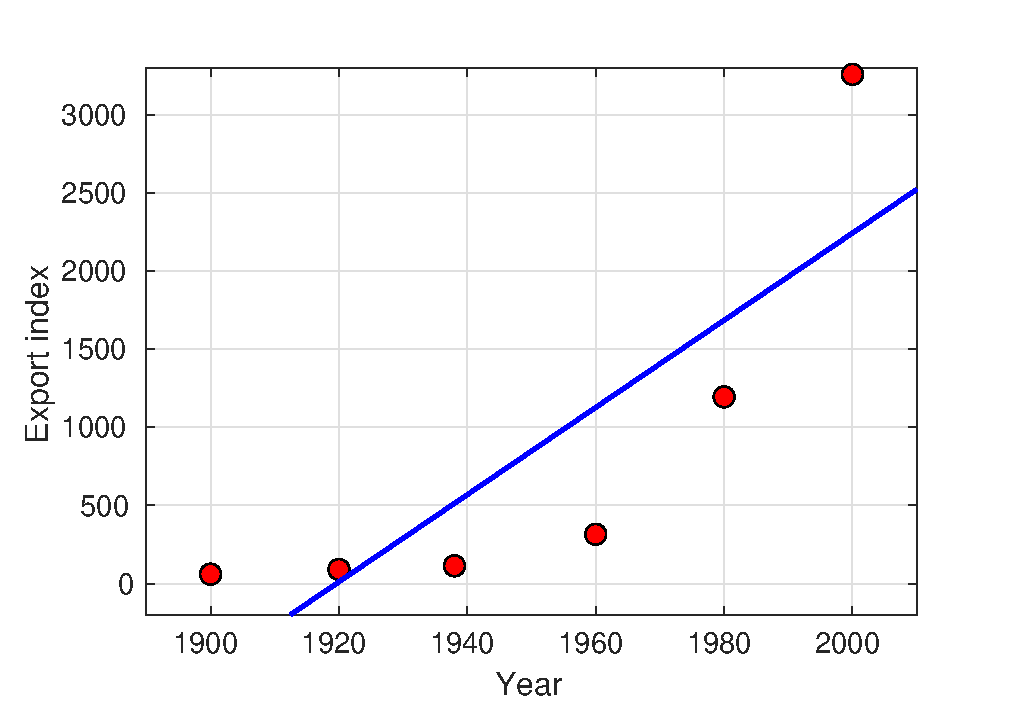
\includegraphics[width=\textwidth]{figures/lsf_linear}}}%
  {linear fit}%
  {quadratic fit}%
  {cubic fit}%
  {exponential fit}%
  {1}{}{Data source: https://ourworldindata.org/trade-and-globalization}

  
  \qitemMCfour{%
    \mytwocol{Over the last century trade has grown remarkably. The
      following graph shows the value of an world export index over the
      period 1900-2000. We have shown a least square fit. What type of
      fit is it?}%
    {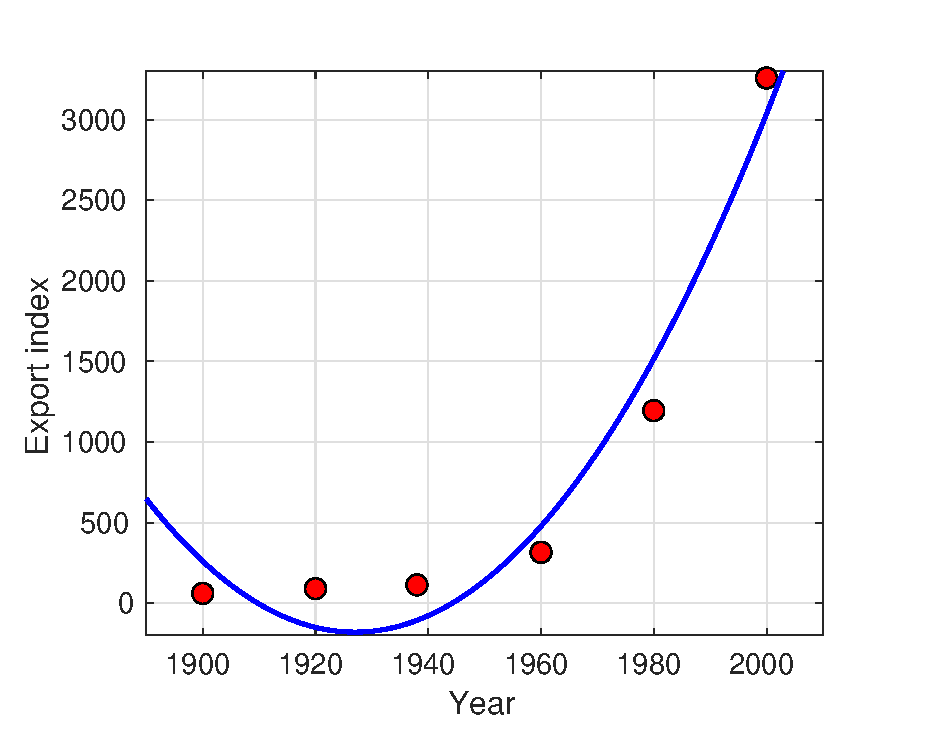
\includegraphics[width=\textwidth]{figures/lsf_quadratic}}}%
  {linear fit}%
  {quadratic fit}%
  {cubic fit}%
  {exponential fit}%
  {2}{}{Data source: https://ourworldindata.org/trade-and-globalization}


  \qitemMCfour{%
    \mytwocol{Over the last century trade has grown remarkably. The
      following graph shows the value of an world export index over the
      period 1900-2000. We have shown a least square fit. What type of
      fit is it?}%
    {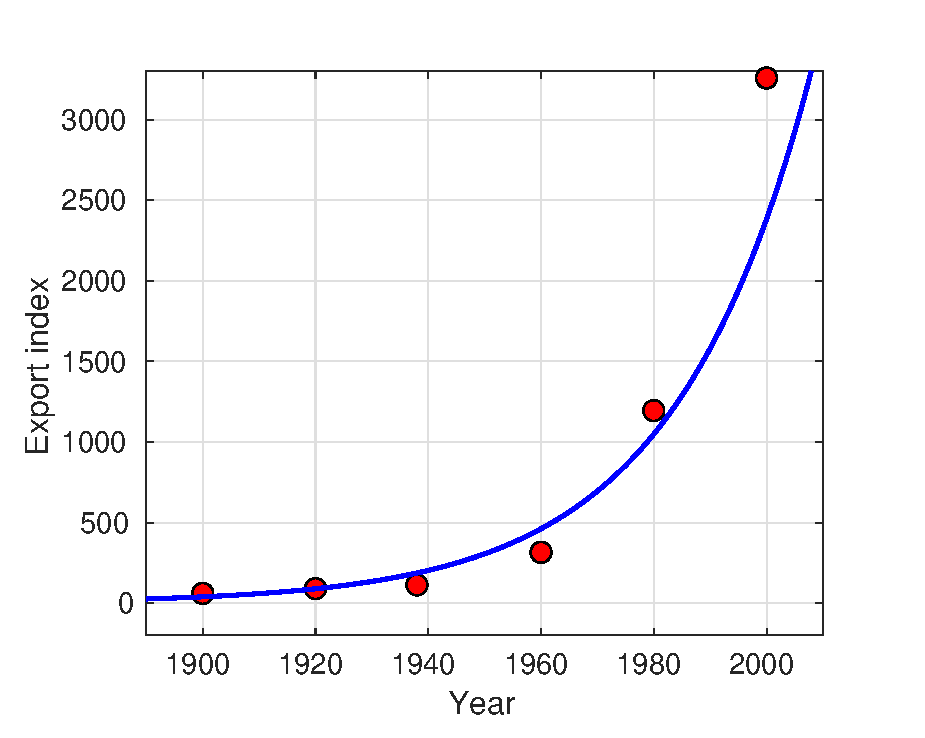
\includegraphics[width=\textwidth]{figures/lsf_exp}}}%
  {linear fit}%
  {quadratic fit}%
  {cubic fit}%
  {exponential fit}%
  {4}{}{Data source: https://ourworldindata.org/trade-and-globalization}  
  
  
  \qitemMCthree{%
    \mytwocol{The plot shows a set of data points along with three
      least-squares fits (numbered 1--3).  The root mean square (RMS)
      errors are listed below:
      \begin{center}
        \begin{tabular}{cc}
          Fit 1: & RMS $=$ 2.8120\\
          Fit 2: & RMS $=$ 1.7655\\
          Fit 3: & RMS $=$ 1.7241
        \end{tabular}
      \end{center}
      Which least-squares fit provides the best match with the data?}%
    {% Matlab code: lsqnoisydata.m
      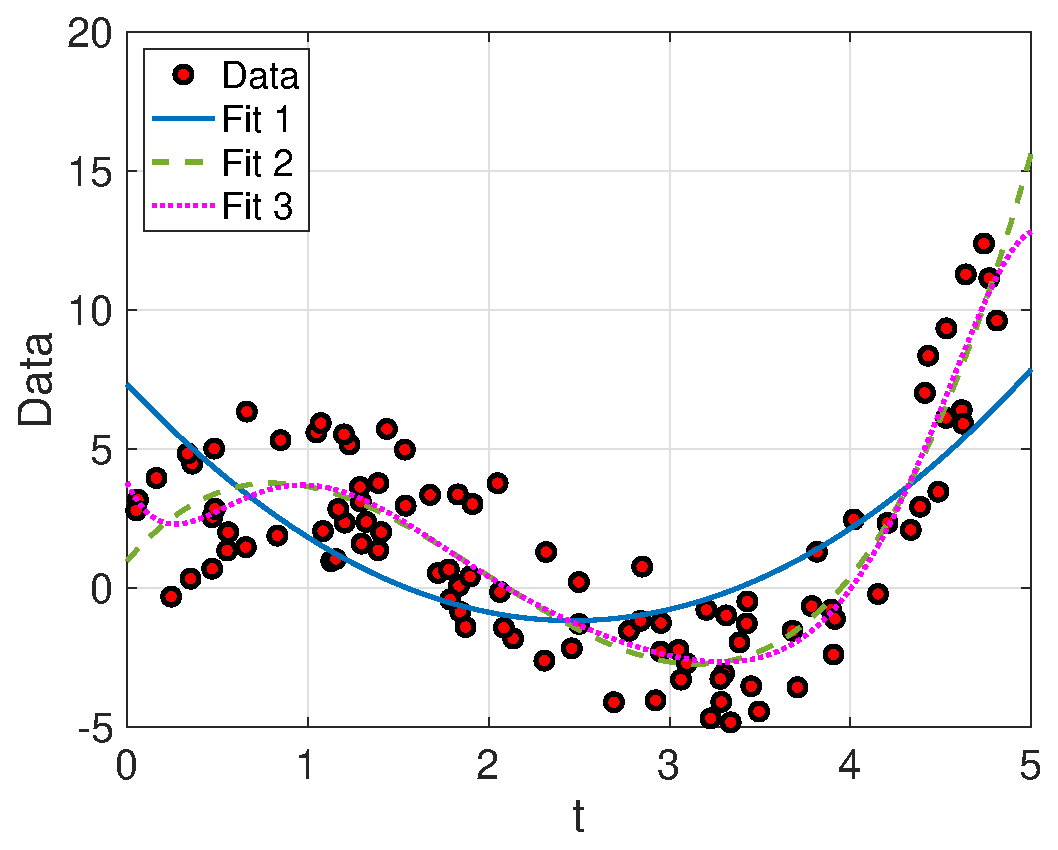
\includegraphics[width=\textwidth]{figures/lsqnoisydata}}}%
  {Fit 1}%
  {Fit 2}%
  {Fit 3}%
  {2}{It would be easy to choose Fit~3 judging by the RMS error alone,
    but the difference from Fit~2 is very small.  So in such cases, it's
    always important to evaluate the fit \myuline{qualitatively} or
    visually \dots\ in the ``eyeball norm''.  Note that Fit~3 exhibits
    some worrying wiggles near the end-points $t=0$ and $5$ that deviate
    from the overall trends in the data.}{\jms}


  \qitemMCfour{\fillblank To find the exponential fit $Q(x) = \alpha
    e^{{\beta} x}$ using a given data set $\{(x_0, y_0), (x_1, y_1),
    \dots, (x_m, y_m)\}$, you can follow these steps:
    \begin{itemize}
      % \item exponential fit $Q(x) = \alpha e^{{\beta} x}$
    \item Take the natural logarithm of both sides
      \begin{gather*}
        \log(Q(x)) = \log(\alpha) + \beta x.
      \end{gather*}
    \item Apply linear least squares to the points \mybigblank to
      obtain the coefficients $a_0 = \log(\alpha)$ and $a_1 = \beta$.
    \item Then $\alpha = e^{a_0}$ and $\beta = a_1$ and $Q(x) = e^{a_0}
      e^{a_1 x}$.
    \end{itemize}}%
  {$\{(x_0, y_0), \; (x_1, y_1), \;\dots,\; (x_m, y_m)\}$}%
  {$\{(\log(x_0), \; \log(y_0)), \; (\log(x_1), \log(y_1)), \; \dots, \;
    (\log(x_m), \log(y_m))\}$}%
  {$\{(\log(x_0), y_0), \; (\log(x_1), y_1), \; \dots, \; (\log(x_m),
    y_m)\}$}% 
  {$\{(x_0, \log(y_0)), \; (x_1, \log(y_1)),\; \dots,\; (x_m,
    \log(y_m))\}$}% 
  {4}{}{\jms, \courseID lecture notes}  
  

  \qitemMCfour{\fillblank To find the power-law fit $Q(x) = \alpha
    x^{\beta}$ using a given data set $\{(x_0, y_0), (x_1, y_1), \dots,
    (x_m, y_m)\}$, you can follow these steps:
    \begin{itemize}
      % \item exponential fit $Q(x) = \alpha x^{\beta}$
    \item Take the natural logarithm of both sides
      \begin{gather*}
        \log(Q(x)) = \log(\alpha) + \beta \log(x).
      \end{gather*}
    \item Apply linear least squares to the points \mybigblank to
      obtain the coefficients $a_0 = \log(\alpha)$ and $a_1 = \beta$. 
    \item Then $\alpha = e^{a_0}$ and $\beta = a_1$ and $Q(x) = e^{a_0}
      x^{a_1}$. 
    \end{itemize}}%
  {$\{(x_0, y_0), \; (x_1, y_1), \;\dots,\; (x_m, y_m)\}$}%
  {$\{(\log(x_0), \log(y_0)), \; (\log(x_1), \log(y_1)), \;\dots,\;
    (\log(x_m), \log(y_m))\}$}% 
  {$\{(\log(x_0), y_0), \; (\log(x_1), y_1), \;\dots,\; (\log(x_m),
    y_m)\}$}% 
  {$\{(x_0, \log(y_0)), \; (x_1, \log(y_1)), \;\dots,\; (x_m,
    \log(y_m))\}$}% 
  {2}{}{\jms, \courseID lecture notes}


  \qitemMCfour{\mbox{}
    To find the exponential fit $Q(x) = \alpha e^{{\beta} x}$ using a
    given data set $\{(x_0, y_0), (x_1, y_1), \dots, (x_m, y_m)\}$, the
    sum of squared residuals to be minimized is}% 
  {$\sum\limits_{i=1}^m\left(y_i - \alpha e^{\beta x_i}\right)^2$}%
  {$\sum\limits_{i=1}^m\left(\log(y_i) - \alpha -\beta x_i\right)^2$}%
  {$\sum\limits_{i=1}^m\left(\log(y_i) - \alpha - \beta \log(x_i)\right)^2$}%
  {$\sum\limits_{i=1}^m\left(\log(y_i) - \log(\alpha) - \beta x_i\right)^2$}%
  {4}{Taking the $\log$ of both sides of the exponential fit 
    \begin{gather*}
      Q(x) = \alpha e^{{\beta} x}
    \end{gather*}
    gives
    \begin{gather*}
      \log(Q(x)) = \log(\alpha) + {\beta} x \implies \log(y_i) =
      log(\alpha) + {\beta} x_i \implies E_i = \log(y_i) - \log(\alpha)
      - {\beta} x_i
    \end{gather*}
    The sum of the square of the residuals
    \begin{gather*}
      \sum\limits_{i=1}^{m} E_i^2 = \sum\limits_{i=1}^m\left(\log(y_i) -
        \log(\alpha) -  {\beta} x_i\right)^2.
    \end{gather*}}{Holistic Numerical Methods~\cite{kaw-2019}} 
  

  \qitemMCfour{\mbox{}
    To find the power law fit $Q(x) = \alpha x^{{\beta}}$ using a given
    data set $\{(x_0, y_0), (x_1, y_1), \dots, (x_m, y_m)\}$, the sum of
    squared residuals to be minimized is}% 
  {$\sum\limits_{i=1}^m\left(y_i - \alpha x_i^{\beta}\right)^2$}%
  {$\sum\limits_{i=1}^m\left(\log(y_i) - \alpha -\beta x_i\right)^2$}%
  {$\sum\limits_{i=1}^m\left(\log(y_i) - \alpha - \beta \log(x_i)\right)^2$}%
  {$\sum\limits_{i=1}^m\left(\log(y_i) - \log(\alpha) - \beta x_i\right)^2$}%
  {3}{Taking the $\log$ of both sides of the exponential fit 
    $Q(x) = \alpha x^{{\beta}}$ gives
    \begin{gather*}
      \log(Q(x)) = \log(\alpha) +  {\beta} \log(x) \implies \log(y_i) =
      \log(\alpha) +  {\beta} \log(x_i) \implies E_i = \log(y_i) -
      \log(\alpha) -  {\beta} \log(x_i)
    \end{gather*}
    The sum of the square of the residuals
    \begin{gather*}
      \sum\limits_{i=1}^{m} E_i^2 = \sum\limits_{i=1}^m\left(\log(y_i) -
        \log(\alpha) -  {\beta} \log(x_i)\right)^2.
    \end{gather*}}%
  {Holistic Numerical Methods~\cite{kaw-2019}} 
  

  \qitemMCfour{Suppose you apply the method of least squares to obtain a
    linear fit $y=ax+b$ to the four points $(x_1, y_1)$, $(x_2, y_2)$,
    $(x_3, y_3)$ and $(x_4, y_4)$.  You then repeat the process by
    fitting the same data points to a function of the form $x=cy+d$.
    Which of the following statements is FALSE?}%
  {The two fitted lines are identical}%
  {The two linear fits may be different}%
  {The procedure fails when $ac = 0$}%
  {$\ds{a=\frac{1}{c}}$}%
  {2}{The first fit minimizes the (vertical) difference in the $y$-values,
    while the second fit minimizes the (horizontal) difference in the
    $x$-values.}{\jms} 

\end{clicklist}


%%%%%%%%%%%%%%%%%%%%%%%%%%%%%%%%%%%%%%%%%%%%%%%%%%%%%%%%%%%%%%%%%%%%%%%%%%%%%% 
\mysubhead{4d}{Applications}

\begin{clicklist}

  \qitemMCfour{%
    \mytwocol[0.5]{A robot has to follow a path that passes through
      seven planning points in order to avoid two obstacles, as shown in
      the plot.  To find the shortest path that is also smooth, which of
      the following solution strategies would you recommend?}%
    {% Maple code: robotpath.m
      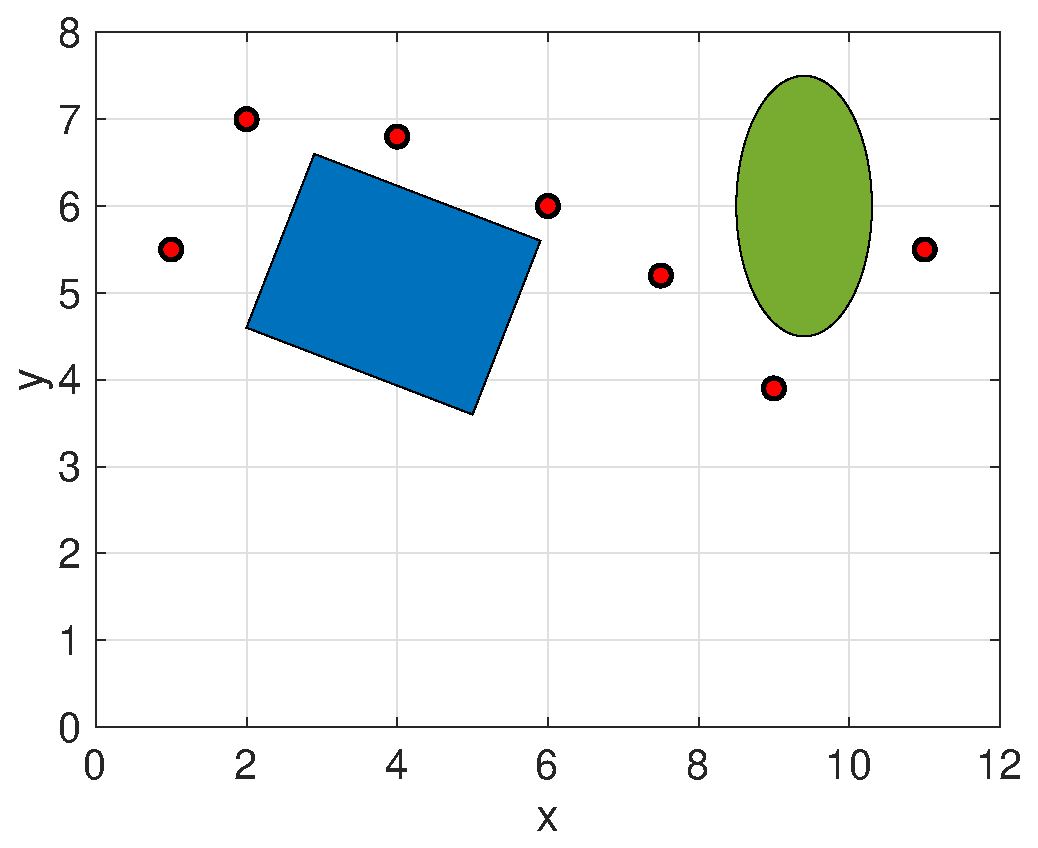
\includegraphics[width=\textwidth]{figures/robotpath}}}%
  {Pass a sixth degree polynomial through the data}%
  {Pass linear splines through the data}%
  {Pass cubic splines through the data}%
  {Use least squares to fit a second degree polynomial}%
  {3}{Linear splines would certainly give the shortest possible path,
    but then the path isn't smooth (maybe not the best for a robot).  A
    least squares fit doesn't interpolate the points and so it's of no
    use.  Among the remaining two choices, (A) is likely to be more
    ``wiggly'' and so will either generate a longer path or run into one
    of the objects.}{\jms}


  \qitemMCfour{%
    \mytwocol[0.35]{If you have ever watched an SFU convocation ceremony,
      then you have no doubt observed the students, faculty and SFU Pipe
      Band process through the Academic Quadrangle and over the
      reflecting pool.  What you may not realize is the fear this event
      strikes in the hearts of its participants, where one tiny misstep
      on the treacherous pond walk can turn a beautiful day into
      disaster.
      \begin{center}
        %\includegraphics[width=\textwidth]{figures/sfuaerial1}
        \includegraphics[width=\textwidth]{figures/sfupondwalk5}%2,3,5
      \end{center}}%
    {% Maple code: sfuquad.m
      \includegraphics[width=\textwidth]{figures/sfuquad1}}
    
    In order to help graduands in selecting a safe procession path, you
    have taken GPS measurements of nine strategically-placed points
    along the procession route.  To determine the safest path over the
    pool, which of the following strategies would you recommend?}%
  {Pass an eighth degree interpolating polynomial through all data points}%
  {Use a linear spline to interpolate the data}%
  {Use a cubic spline to interpolate the data}%
  {Use least squares to fit a third degree polynomial}%
  {3}{\begin{center}
      \includegraphics[width=0.35\textwidth]{figures/sfuquad2}
    \end{center}}{\mah\ and \jms}
  
\end{clicklist}

%%%%%%%%%%%%%%%%%%%%%%%%%%%%%%%%%%%%%%%%%%%%%%%%%%%%%%%%%%%%%%%%%%%%%%%%%%%%%% 
\newpage
\myhead{5}{Differentiation and Integration}
\mysubhead{5a}{Numerical Differentiation}

\begin{clicklist}
  
  \leavethisout{
    \qitemMCfour{Which of the following statements is the definition for
      the first derivative of a function $f(x)$?}%
    {$\ds{f'(x) = \lim_{h \to 0}\frac{f(x+h) - f(x)}{h}}$}%
    {$\ds{f'(x) = \lim_{h \to 0}\frac{f(x+h) + f(x)}{h}}$}%
    {$\ds{f'(x) = \frac{f(x+h) - f(h)}{h}}$}%
    {All of the above}%
    {1}{}{\mah}
  }

  \qitemMCfour{Which of the following limit statements regarding 
    the first derivative of a smooth function $f(x)$ is TRUE?}%
  {$\ds{f'(x) = \lim_{h \to 0}\frac{f(x+h) - f(x)}{h}}$}%
  {$\ds{f'(x) = \lim_{h \to 0}\frac{f(x-h) - f(x)}{-h}}$}%
  {$\ds{f'(x) = \lim_{h \to 0}\frac{f(x+h) - f(x-h)}{2h}}$}%
  {All of the above}%
  {4}{}{\mah}

  
  \qitemMCfour{Which of the following difference formulas is a
    valid approximation of $f'(x_i)$?  Here, the $x_i$ represent
    equally-spaced points with $x_i - x_{i-1} = h$.}%
  {$\ds{\frac{f(x_{i+1}) - f(x_i)}{h}}$}%
  {$\ds{\frac{f(x_i) - f(x_{i-1})}{h}}$}%
  {$\ds{\frac{f(x_{i+1}) - f(x_{i-1})}{2h}}$}%
  {All of the above}%
  {4}{}{\mah}

              
  \qitemMCfour{What form does the truncation error take for the
    difference formula $\ds{f'(x) \approx \frac{f(x+h) -
        f(x-h)}{2h}}$~?}%
  {$O(1)$}%
  {$O(h)$}%
  {$O(2h)$}%
  {$O(h^2)$}%
  {4}{}{\mah}
  

  \qitemMCfour{How would you classify the following difference formula
    for the derivative
    \begin{gather*}
      f'(x) \approx \frac{-3f(x) + 4f(x+h) - f(x+2h)}{2h} \; \text{?}   
    \end{gather*}}%
  {forward difference}%
  {backward difference}%
  {centered difference}%
  {one-sided difference}%
  {4}{You can also think of this as a forward difference formula, in the
    sense that the stencil consists of points located ``forward'' of the
    approximation point $x$, so response (A) is equally valid.}{\mah}


  \qitemMCfour{You want to estimate the first derivative of
    $f(x)$, given values of the function at discrete points $x = 0, 0.1,
    0.2, \dots, 1$. Which of these formulas is appropriate for 
    estimating $f'(1)$?}%
  {$\ds{f'(x) \approx \frac{-3f(x) + 4f(x+h) - f(x+2h)}{2h}}$}%
  {$\ds{f'(x) \approx \frac{f(x+h) - f(x-h)}{2h}}$}%
  {$\ds{f'(x) \approx \frac{3f(x) - 4f(x-h) + f(x-2h)}{2h}}$}%
  {All of the above}%
  {3}{The other two involve points $x=1.1$ or $x=1.2$ where $f$ is not
    known.}{\mah}
  
  
  \qitemMCfour{You want to estimate the first derivative of
    $f(x)$, given values of the function at discrete points $x_0, x_1,
    x_2, \dots, x_n$. Which of these formulas is appropriate for
    estimating $f'(x_0)$?}%
  {$\ds{f'(x_i) \approx \frac{-3f(x_i) + 4f(x_{i+1}) - f(x_{i+2})}{2h}}$}%
  {$\ds{f'(x_i) \approx \frac{f(x_{i+1}) - f(x_{i-1})}{2h}}$}%
  {$\ds{f'(x_i) \approx \frac{3f(x_i) - 4f(x_{i-1}) + f(x_{i-2})}{2h}}$}%
  {All of the above}%
  {1}{The other two involve points to the left of $x_0$ where $f$ is not
    known.}{\mah}

  
  \leavethisout{
    \qitemTF{\begin{gather*}
        f'(x) = \frac{1}{12h}\left(f(x-2h) - 8f(x-h) + 8f(x+h) -
          f(x+2h)\right) + \frac{h^4}{30}f^{(5)}(c)
      \end{gather*}
      This is a 4-point centered formula.}%
    {FALSE}{This is a 5-point $\{x-2h, x-h, x, x+h, x+2h\}$ centered
      formula.}{\mah}
  }
  
  \qitemMCfour{Which of the statements below is TRUE regarding the
    difference formula
    \begin{gather*}
      f'(x) = \frac{1}{12h} \Big[ f(x-2h) - 8f(x-h) + 8f(x+h) - f(x+2h)
      \Big] + \frac{h^4}{30}\, f^{(5)}(c) \; \text{?}
    \end{gather*}}%
  {it is a 5-point centered formula}%
  {the truncation error is $O(h^4)$}%
  {when $h$ is large, the truncation error dominates}%
  {All of the above}%
  {4}{Regarding response (A): this formula spans a five-point
    stencil centered at the approximation point $x$, but the coefficient
    multiplying $f(x)$ is zero.}{} 
  

  \qitemMCfour{%
    \mytwocol{The given table lists the absolute errors from three
      finite difference approximations of the derivative $f'(x)$
      (labelled A, B, C).  The errors are computed for a
      sequence of decreasing values of the grid spacing $h$.\\

      Which of the statements below regarding the order of
      accuracy for the three formulas is TRUE?}%
    {% Table from 'deriv1.m'
      {\tt\small
        \begin{tabular}{c|ccc}
          h & Formula A & Formula B & Formula C\\\hline
          0.500000 & 5.764e-01 & 6.670e-02 & 9.329e-03\\
          0.250000 & 3.096e-01 & 1.683e-02 & 3.565e-04\\
          0.125000 & 1.596e-01 & 4.218e-03 & 5.181e-05\\
          0.062500 & 8.093e-02 & 1.055e-03 & 4.116e-06\\
          0.031250 & 4.074e-02 & 2.638e-04 & 2.836e-07\\
          0.015625 & 2.044e-02 & 6.595e-05 & 1.853e-08\\
          0.007812 & 1.024e-02 & 1.649e-05 & 1.183e-09\\
          0.003906 & 5.122e-03 & 4.122e-06 & 7.513e-11
        \end{tabular}}}}%
  {Formulas~A and~B are order~1, Formula~C is order~2.}%
  {Formula~A is order~1, Formula~B is order~2, Formula~C is order~3.}%
  {Formula~A is order~1, Formula~B is order~2, Formula~C is order~4.}%
  {All formulas have the same order of accuracy, but different error
    constants.}%
  {3}{Notice first that $h$ is reduced by a factor of 2 in each step.
    Then observe that the error in Formula~A goes down roughly by a
    factor of $2$ in each step, Formula~B by $4=2^2$, and Formula~C by
    $16=2^4$.}{\jms}


  \qitemMCfour{%
    \mytwocol{The given table lists approximations for $f'(x)$ using
      three finite difference formulas (labelled A, B, C).  The
      approximations are computed for a sequence of decreasing values of
      the grid spacing $h$.\\
      
      Consider the convergence of the approximations as $h\to 0$, and
      notice that the some of the results behave anomalously for the
      smallest values of $h$.  What is the most likely explanation for
      this behaviour?}%
    {% Table from 'deriv2.m'
      {\tt\small
        \begin{tabular}{c|ccc}
          h & Formula A & Formula B & Formula C\\\hline
          1.0e-00 &  2.474412954 & 1.263946140 & 1.974278619\\
          1.0e-01 &  1.649322255 & 1.518206757 & 1.520883362\\
          1.0e-02 &  1.534001862 & 1.520879903 & 1.520906914\\
          1.0e-03 &  1.522218854 & 1.520906647 & 1.520906918\\
          1.0e-04 &  1.521038136 & 1.520906915 & 1.520906918\\
          1.0e-05 &  1.520920040 & 1.520906918 & 1.520906918\\
          1.0e-06 &  1.520908230 & 1.520906918 & 1.520906917\\
          1.0e-07 &  1.520907045 & 1.520906916 & 1.520906919\\
          1.0e-08 &  1.520906956 & 1.520906934 & 1.520906645\\
          1.0e-09 &  1.520906512 & 1.520906956 & 1.520908177\\
          1.0e-10 &  1.520903403 & 1.520905624 & 1.520903403\\
          1.0e-11 &  1.520916726 & 1.520916726 & 1.520794601\\
          1.0e-12 &  1.520561455 & 1.520783499 & 1.520672477\\
          %1.0e-13 &  1.523225990 & 1.521005544 & 1.485478407\\
          %1.0e-14 &  1.509903313 & 1.509903313 & 1.454392162\\
          %1.0e-15 &  1.332267630 & 1.332267630 & 0.555111512\\
          %1.0e-16 &  0.000000000 & 0.000000000 &-24.424906542
        \end{tabular}}}}%
  {Formula~A converges with first order accuracy, while Formulas~B and~C
    diverge.}%
  {All three formulas suffer from subtractive cancellation errors for
    small enough $h$.}%
  {Local truncation error dominates at small $h$, and is largest for
    Formula~C.}%
  {Convergence stalls for Formulas~B and~C around $h\approx 10^{-5}$, but
    then resumes when $h$ gets small enough.}%
  {2}{Difference formulas are just that -- differences -- and so they
    experience subtractive cancellation errors when $h$ is small and
    function values get very close to each other.  These errors are then
    magnified by a factor of $\frac{1}{h}$.  As an example, consider the
    first-order one-sided difference formula $\frac{f(x)-f(x-h)}{h}$
    (this is Formula~A).
    % Formulas B and C are definitely starting to
    % \myuline{diverge} when $h$ is smaller than $10^{-5}$. 
  }{\jms}


  \qitemMCfour{An electric circuit contains a resistor (resistance $R$),
    an inductor (inductance $L$) and a variable voltage source $E(t)$
    that obeys
    \begin{gather*}
      E(t) = L \frac{di}{dt} + Ri, 
    \end{gather*}
    where $i(t)$ is the electric current flowing through the
    circuit. You have measurements of current at several times:
    \begin{center}
      \begin{tabular}{l|c|c|c|c} 
        time, $t$ (seconds)    & 1.00 & 1.01 & 1.05 & 1.10 \\
        \hline
        current, $i$ (amperes) & 4.01 & 4.05 & 4.10 & 4.50 \\
      \end{tabular}
    \end{center}
    If the inductance is $L = 0.82$ henries and the resistance is $R =
    0.21$ ohms, the most accurate approximation for $E(1.10)$ is}%
  {$\ds{0.82\left(\frac{4.50 - 4.10}{0.05}\right) + 0.21(4.50)}$}%
  {$0.21(4.50)$}%
  {$\ds{0.82\left(\frac{4.05 - 4.01}{0.01}\right) + 0.21(4.50)}$}%
  {$\ds{0.82\left(\frac{4.50 - 4.01}{0.1}\right) + 0.21(4.50)}$}%
  {1}{This uses a backward approximation to $i'(1.1)$ that uses the
    points closest to $x=1.1$. Response (D) uses a higher order centered
    approximation of the derivative, but it's centered at the wrong
    point -- $x=1.055$!}{Holistic Numerical Methods~\cite{kaw-2019} and
    Burden \& Faires~\cite{burden-faires-2015}, p.~182}
  

  \qitemMCfour{The table below lists the distance $s(t)$ that a
    car travels along a straight road in time $t$:
    \begin{center}
      \begin{tabular}{c|c|c|c|c} 
        Time, $t$ (seconds) & 0 & 5 & 10 & 15 \\
        \hline
        Distance, $s$ (m) & 0  & 100 & 300 & 700 \\
      \end{tabular}
    \end{center}
    Using the forward, backward or centered difference approximation,
    what is the best estimate you can find for the velocity
    $v=\frac{ds}{dt}$ of the car at $t=10$ seconds?}%
  {50}%
  {60}%
  {100}%
  {200}%
  {2}{The centered difference approximation gives $\ds{v(10) \approx
      \left(\frac{700 - 100}{15-5}\right)=60}$.}{Holistic Numerical
    Methods~\cite{kaw-2019} and Burden \&\
    Faires~\cite{burden-faires-2015}, p.~182}

  
  \qitemMCfour{In the following centered difference formula for the
    second derivative
    \begin{gather*}
      f''(x) = \frac{1}{12h^2} \Big[ A f(x-2h) + 16f(x-h) - 30f(x) +
        16f(x+h) + A f(x+2h) \Big] + O(h^4),
    \end{gather*}
    what must the constant $A$ be for the formula to be correct?}%
  {$-1$}%
  {$1$}%
  {$-2$}%
  {$2$}%
  {1}{You could answer this by expanding in Taylor series.  But it's
    easier to simply recall that in any difference approximation of a
    derivative, the stencil coefficients must sum to zero.  Then 
    $A+16-30+16+A = 0$.}{\mah}
  

  \qitemMCfour{A first-order difference approximation of the first
    derivative is written in the form $f'(x) = G(h) + a \cdot h +
    O(h^2)$, where $a$ is some constant. Which of the extrapolation
    formulas below is an $O(h^2)$ approximation of $f'(x)$?}%
  {$\ds{\frac{4 G\left(\frac{h}{2}\right) - G(h)}{3}}$}%
  {$\ds{\frac{2 G\left(\frac{h}{2}\right) - G(h)}{3}}$}%
  {$\ds{2G\left(\frac{h}{2}\right) - G(h)}$}%
  {none of the above}%
  {3}{This is analogous to Richardson extrapolation, just applied to an
    $O(h)$ formula.}{\mah}
  

  \qitemMCfour{\fillblank The truncation error terms in a difference
    approximation $G(h)$ for the first derivative of a function can be
    written as $f'(x) = G(h) + a_1 h + a_2 h^2 + a_3 h^2 + \dots$.  Then
    one step of extrapolation can be used to write $f'(x) =
    2G\left(\frac{h}{2}\right) - G(h) + O(h^2)$.  Applying one more
    extrapolation step yields the next higher order formula $f'(x) =
    \mybigblank + O(h^3)$.}%
  {$\ds{\frac{4G\left(\frac{h}{2}\right) - G(h)}{3}}$}%
  {$\ds{\frac{8G\left(\frac{h}{4}\right) -
        G\left(\frac{h}{2}\right)}{3}}$}%
  {$\ds{\frac{8G\left(\frac{h}{4}\right) + G(h)}{3}}$}%
  {$\ds{\frac{8G\left(\frac{h}{4}\right) - 6G\left(\frac{h}{2}\right) +
        G(h)}{3}}$}%
  {4}{}{\mah}
  

  \qitemMCfour{Write the truncation error terms in the centered
    difference approximation for the first derivative as
    \begin{gather*}
      f'(x) = \frac{f(x+h) - f(x-h)}{2h} + a_1 h^2 + a_2 h^4 + a_3 h^6 +
      \dots
    \end{gather*}
    where the $a_i$ are constants.  After applying \myuline{$n$ steps}
    of Richardson extrapolation, what is the order of the resulting
    approximation for $f'(x)$?}%
  {$O(h^2)$}%
  {$O(h^n)$}%
  {$O(h^{2n})$}%
  {$O(h^{2n+2})$}%
  {4}{Each step increases the order by a factor of $h^2$ so the error is
    $O(h^2 \cdot (h^{2})^n) = O(h^{2n+2})$.}{\mah}
  
\end{clicklist}

%%%%%%%%%%%%%%%%%%%%%%%%%%%%%%%%%%%%%%%%%%%%%%%%%%%%%%%%%%%%%%%%%%%%%%%%%%%%%%
\mysubhead{5b}{Numerical Integration or Quadrature}

\begin{clicklist}
  \qitemMCfour{The Fundamental Theorem of Calculus is}%
  {$\ds{\int_a^b f(x)\, dx = f(b) - f(a)}$}%
  {$\ds{\int_a^b f(x)\, dx = F(b) - F(a)}$ where $f'(x) = F(x)$}%
  {$\ds{\int_a^b f(x)\, dx = F(b) - F(a)}$ where $F'(x) = f(x)$}%
  {$\ds{\int_a^b f(x)\, dx = \frac{f(b)-f(a)}{b-a}}$}%
  {3}{In the theorem statement, $F$ is an antiderivative and so $F'=f$.}{}


  \qitemMCfour{The definite integral $\ds{\int_a^b f(x)\, dx}$ can be
    interpreted as \dots}%
  {the average value of $f(x)$ on the interval $[a,b]$}%
  {the area under the curve $y = f(x)$ between $x=a$ and $x=b$}%
  {the work done by a force $f(x)$ that acts on an object moving from
    position $x=a$ to $b$}%
  {all of the above}%
  {2}{Both (B) and (C) are valid interpretations.  Response (A) might
    also be correct, but only if $b-a=1$ since the \myuline{average}
    value of a function is defined as $\frac{1}{b-a}\int_a^b f(x)\,
    dx$.}{\jms, \courseID lecture notes}
  
  
  \qitemMCfour{The definite integral $\ds{\int_a^b f(x)\, dx}$ can be
    interpreted as}%
  {the area below the curve $y = f(x)$ from $a$ to $b$}%
  {the area above the curve $y = f(x)$ from $a$ to $b$}%
  {the difference in end-point values, $f(b) - f(a)$}%
  {the arithmetic average, $\ds{\frac{f(a) + f(b)}{2}}$}%
  {1}{Response (A) is correct, but only as long as $f(x)$ is positive on
    $[a,b]$. Wherever $f(x)$ is negative, then (B) is the correct
    interpretation.}{\mah}
  
  
  \qitemMCfour{The average value of $f(x)$ on $[a,b]$ is}%
  {$\ds{\frac{f(a) + f(b)}{2}}$}%
  {$\ds{\frac{f(a) + f(b)}{a+b}}$}%
  {$\ds{\int_a^b f(x)\, dx}$}
  {$\ds{\frac{1}{b-a} \int_a^b f(x)\, dx}$}%
  {4}{}{Adapted from Holistic Numerical Methods~\cite{kaw-2019}, {\tt
      quiz\_07\_01}} 


  \qitemTF{The left and right rectangle rules are exact for constant
    functions, $f(x) = c$.}%
  {TRUE}{}{\jms, \courseID lecture notes}
            

  \qitemMCfour{Which of the statements below is TRUE? Trapezoidal
    rule is exact for:
    \begin{IVlist}
    \item constant functions, $f(x) = c$
    \item linear functions, $f(x) = ax + b$
    \item quadratic functions, $f(x) = ax^2 + bx + c$
    \end{IVlist}}%
  {I}%
  {II}%
  {I and II}%
  {I, II and III}%
  {3}{}{\jms, \courseID lecture notes}


  \qitemMCfive{Which of the following statements is TRUE?
    \begin{IVlist}
    \item Simpson's rule is exact for linear functions, $f(x) = ax + b$.
    \item Simpson's rule is exact for second-degree polynomials
      (quadratics), $f(x) = ax^2 + bx + c$.
    \item Simpson's rule is exact for fourth-degree polynomials.
    \end{IVlist}}%
  {none is true}%
  {I}%
  {II}%
  {I and II}%
  {I, II and III}%
  {4}{}{\jms, \courseID lecture notes}


  % Fun historical fact
  \qitemMCthree{Numerical integration is called ``quadrature'' because
    \dots}%
  {it is exact for quadratic functions.}%
  {the Greeks conceived of computing the area of a complex shape by
    replacing it with a square having the same area, and ``quad'' $\sim$
    square.}%
  {the simplest formulas involve dividing up the area into quadrangles,
    which are just rectangles (the Latin word \emph{quadrangulum} means
    ``four-cornered''.)}%
  {2}{This is what Wikipedia tells us, but (C) has got to be a
    reasonable explanation as well!}{\jms}

  
  \qitemMCfour{%
    \mytwocol{The integral $\int\limits_0^5 f(x)\, dx$ is approximated
      using the left rectangle rule ($A_L$), right rectangle rule
      ($A_R$) and midpoint rule ($A_M$) for the function $f(x)$ shown in
      the plot.\\

      Which of the following inequalities must be TRUE?}%
    {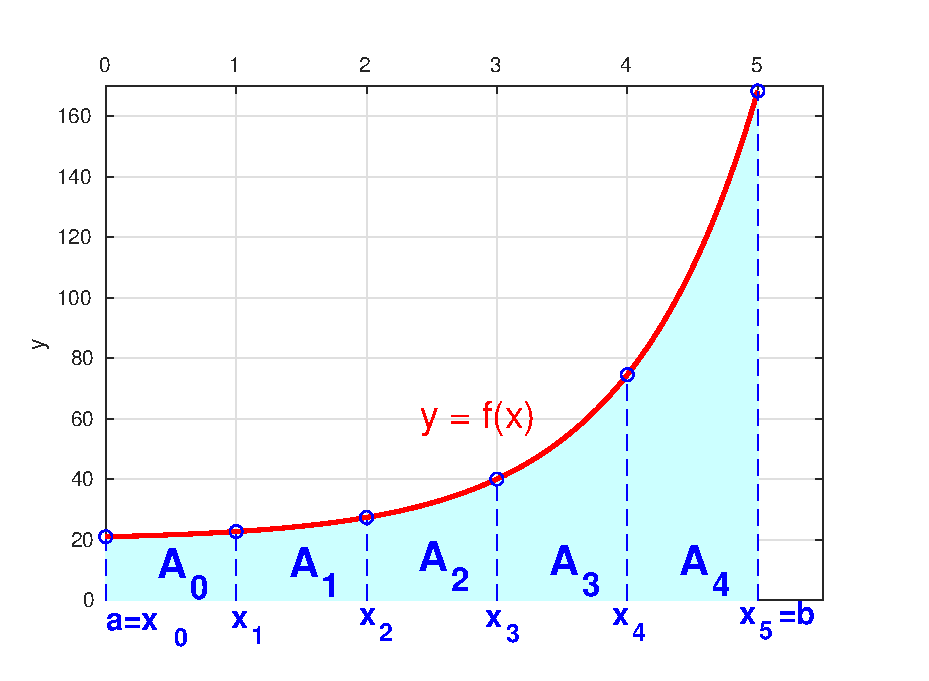
\includegraphics[width=\textwidth]{figures/trap2}}}%
  {$A_L < A_M < A_R$}%
  {$A_M < A_L < A_R$}%
  {$A_R < A_M < A_L$}%
  {$A_M < A_R < A_L$}%
  {1}{\mbox{}\\
    \begin{center}
      \begin{tabular}{c@{}c@{}c@{}c@{}c}
        $A_L$ & $<$ & $A_M$ & $<$ & $A_R$\\
        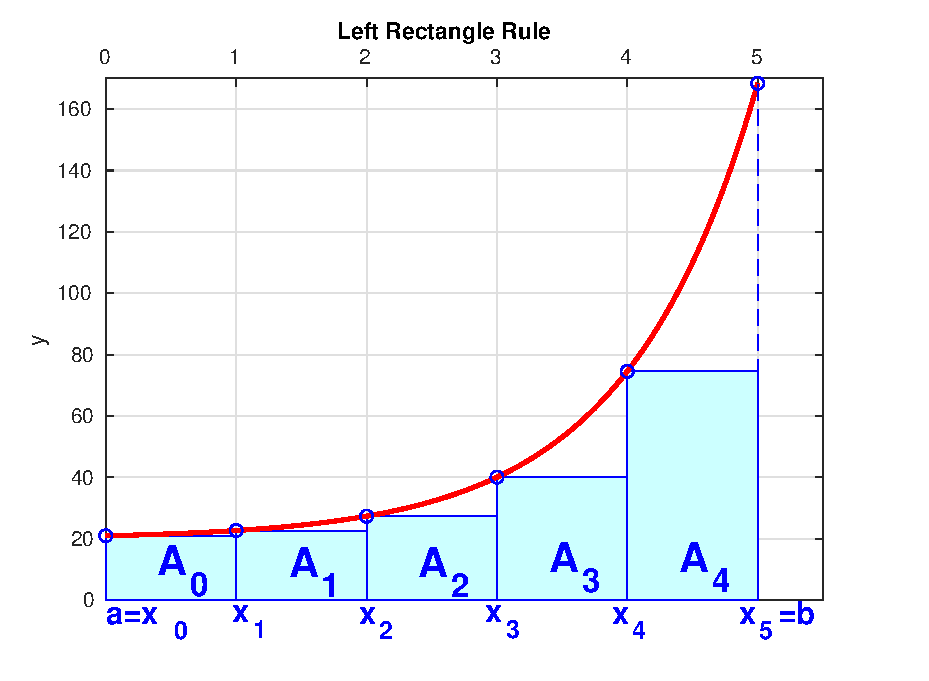
\includegraphics[width=0.31\textwidth]{figures/trap2_1}&&
        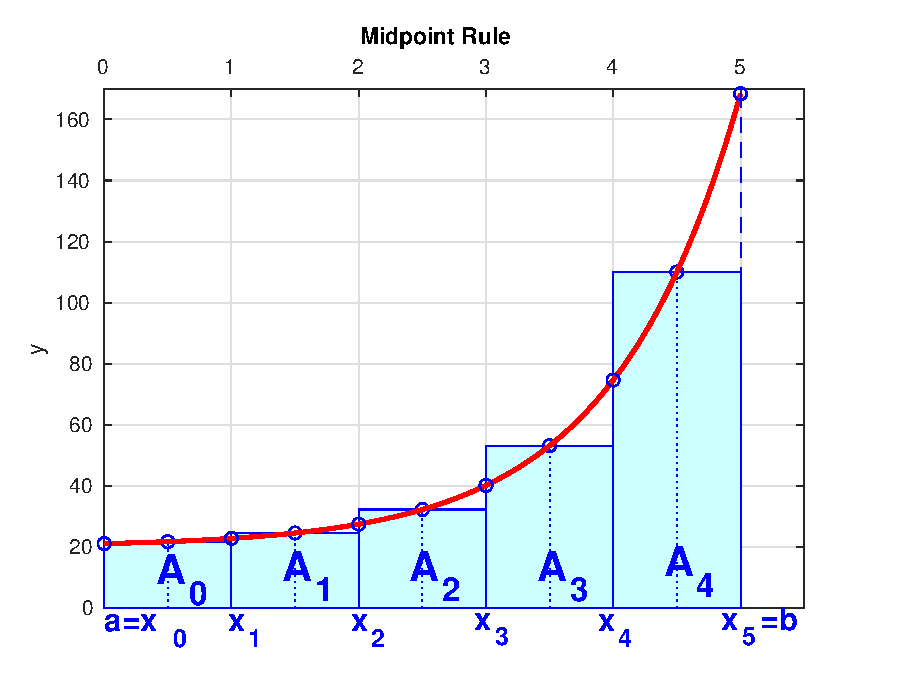
\includegraphics[width=0.3\textwidth]{figures/trap2_3}&&
        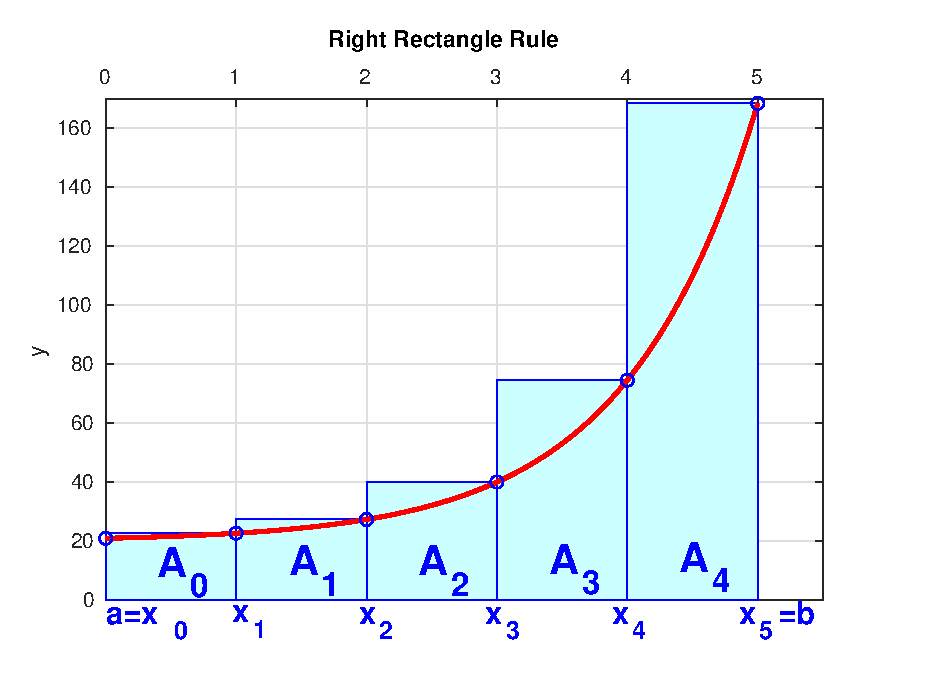
\includegraphics[width=0.32\textwidth]{figures/trap2_2}
      \end{tabular}
    \end{center}}{\mah}

  
  \qitemMCfour{%
    \mytwocol{Apply the trapezoidal rule to approximate the integral
      $A=\int\limits_0^5 f(x)\, dx$ for the given function $f(x)$ shown
      in the plot.\\

      If $A_T$ is the approximation and $A$ is the exact value, which of
      the following relations is TRUE?}%
    {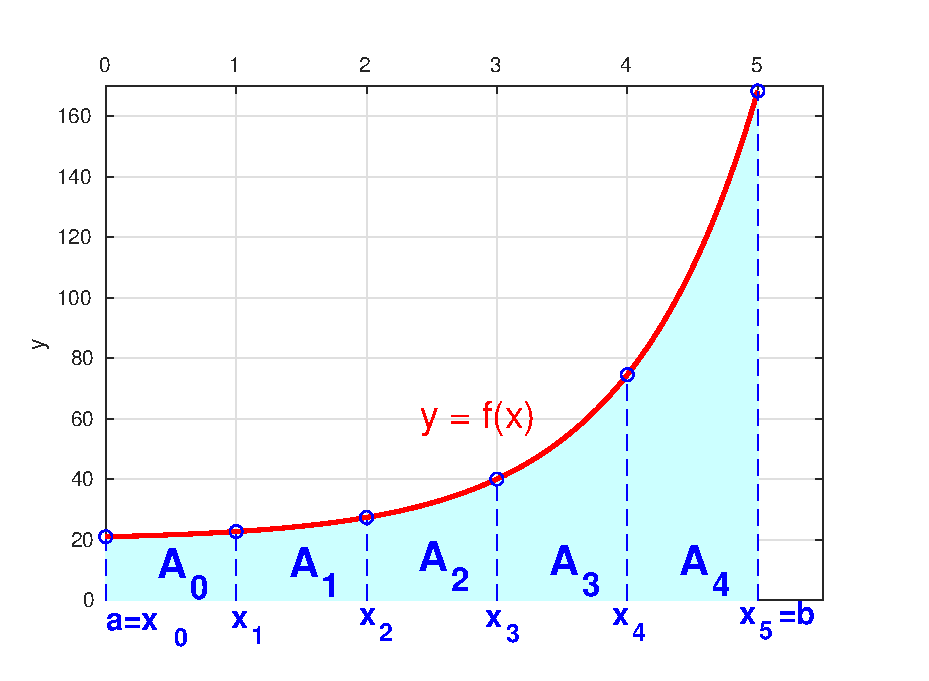
\includegraphics[width=\textwidth]{figures/trap2}}}%
  {$A_T > A$}%
  {$A_T < A$}%
  {$A_T = A$}%
  {none of the above}%
  {1}{The function is concave upwards and so the trapezoidal areas
    (defined by secant lines) always lie slightly above the curve.
    Then $A_T$ is an overestimate of $A$.\\
    \begin{minipage}[t]{\textwidth}
      \begin{center}
        \vspace{0pt}
        \includegraphics[width=0.31\textwidth]{figures/trap2_4}
      \end{center}
    \end{minipage}}{\mah}    
  
  
  \qitemMCfour{%
    \mytwocol{Approximate the integral $A=\int\limits_0^5 f(x)\, dx$
      using the left rectangle rule ($A_L$), right rectangle rule
      ($A_R$) and trapezoidal rule ($A_T$) for the function $f(x)$ shown
      in the plot.\\

      Which of the inequalities below must be TRUE?}%
    {\includegraphics[width=\textwidth]{figures/trap2}}}%
  {$A_L < A_T < A < A_R$}%
  {$A_L < A < A_T < A_R$}%
  {$A_R < A_T < A < A_L$}%
  {$A_T < A_L < A < A_R$}%
  {2}{\mbox{}\\
    \begin{center}
      \begin{tabular}{c@{\hspace*{-10pt}}c@{\hspace*{-10pt}}c@{}c@{}c}
        $A_L$ & $<A<$ & $A_T$ & $<$ & $A_R$\\
        \includegraphics[width=0.3\textwidth]{figures/trap2_1}&&
        \includegraphics[width=0.3\textwidth]{figures/trap2_4}&&
        \includegraphics[width=0.3\textwidth]{figures/trap2_2}
      \end{tabular}
    \end{center}}{\mah}
  
  
  \qitemMCfour{%
    \mytwocol{Approximate the integral $\int\limits_0^9 g(x)\, dx$ using
      the left rectangle rule ($A_L$) and right rectangle rule ($A_R$)
      for the function $g(x)$ shown in the plot.\\

      Which of the following relations is TRUE?}%
    {\includegraphics[width=\textwidth]{figures/trap3}}}%
  {$A_L > A_R$}%
  {$A_L < A_R$}%
  {$A_L = A_R$}%
  {none of the above}%
  {1}{\mbox{}\\
    \begin{center}
      \begin{tabular}{c@{}c@{}c@{}c}
        $A_L$ & $>$ & $A_R$\\
        \includegraphics[width=0.35\textwidth]{figures/trap3_1}&&
        \includegraphics[width=0.35\textwidth]{figures/trap3_2}
      \end{tabular}
    \end{center}}{\mah}
  
  
  \qitemMCfour{%
    \mytwocol{Approximate the integral $A=\int\limits_0^9 g(x)\, dx$
      using the left rectangle rule ($A_L$), right rectangle rule
      ($A_R$) and trapezoidal rule ($A_T$) for the function $g(x)$ shown
      in the plot.\\

      Which of the inequalities below must be TRUE?}%
    {\includegraphics[width=\textwidth]{figures/trap3}}}%
  {$A_L < A_T < A < A_R$}%
  {$A_L < A < A_T < A_R$}%
  {$A_R < A_T < A < A_L$}%
  {$A_T < A_L < A < A_R$}%
  {3}{}{\mah}

  
  \qitemMCfour{Approximate the integral $\int\limits_a^b h(x)\, dx$ using
    the left rectangle rule ($A_L$), right rectangle rule ($A_R$) and
    trapezoidal rule ($A_T$) for some arbitrary function $y=h(x)$. \\

    Which of the following relations must be TRUE?}%
  {$A_L < A_T < A_R$}%
  {$A_R < A_T < A_L$}%
  {$A_R < A_L < A_T$}%
  {$\ds{A_T = \half (A_L + A_R)}$}%
  {4}{The left and right rectangle rules are
    \begin{gather*}
      A_L = h \sum_{i=0}^{n-1} f(x_i) \quad \text{and} \quad
      A_R = h \sum_{i=1}^{n}   f(x_i), \\
      \intertext{and their sum is just}
      A_L + A_R = h \left[ f(x_0) + 2 \sum_{i=1}^{n-1} f(x_i) + f(x_n) \right]
      = 2A_T \quad \text{(implies (D))}      
    \end{gather*}
    Whether inequalities (A), (B) or (C) are true depends on the shape
    of $h(x)$.}{\mah}


  \qitemMCfour{%
    \mytwocol{The given plot shows the absolute error from three
      different quadrature approximations of the integral $\int_a^b
      f(x)\, dx$ (labelled Formulas A, B, C).  The errors are computed
      for a sequence of decreasing values of $h$, the grid
      spacing.\\

      Which of these statements regarding the order of
      accuracy for the three formulas is TRUE?}%
    {% Plot from 'integr1h.m'
      \includegraphics[width=\textwidth]{figures/integr1h}}}%
  {Formulas~A and~B are order~1, Formula~C is order~2.}%
  {Formula~A is order~1, Formula~B is order~2, Formula~C is order~3.}%
  {Formula~A is order~1, Formula~B is order~2, Formula~C is order~4.}%
  {All formulas have the same order of accuracy, but different error
    constants.}%
  {3}{On a log-log scale, the order of the scheme is given by the slope
    of each error curve. For example, with Formula B, $h$ decreases by
    roughly 1000 (3 orders of magnitude) while error decreases by a
    factor of $10^{-6}$ (6 orders of magnitude).  This means that the
    error behaves like $E \propto h^{6/3} \propto h^2$, so
    it's a second-order method.}{\jms}


  \qitemMCfour{%
    \mytwocol{The given plot shows the absolute error in three different 
      quadrature approximations of the integral $\int_a^b f(x)\, dx$
      (labelled Formulas A, B, C).  The errors are computed for a
      sequence of decreasing values of $h$, the grid spacing.\\
      
      Consider the convergence of the approximations as $h\to 0$, and
      notice that there is some odd behaviour with Formula~C.  What is
      the most likely explanation for this behaviour?}%
    {% Plot from 'integr2h.m'
      \includegraphics[width=\textwidth]{figures/integr2h}}}%
  {Formulas~A and B converge with order 1 and 2 respectively, whereas
    Formula~C diverges.}%
  {Formula~C suffers from subtractive cancellation errors when $h$ is
    small enough.}%
  {The accuracy of all three formulas is limited by round-off errors
    that dominate the calculation when $h$ is small.}%
  {There is probably a coding error in Formula~C.}%
  {3}{The error in Formula~C levels off at around $10^{-15}$ which is
    pretty close to machine epsilon in double-precision floating point
    arithmetic. This is an indication that round-off errors are what's
    limiting the accuracy.  Response (B) isn't correct because
    subtractive cancellation errors tend not to occur in quadrature
    formulas, since they generally involve summing terms with mostly the
    same sign.}{\jms}


  \qitemMCfour{The quadrature formula 
    \begin{gather*}
      \int_{0}^1 f(x)\, dx = c_0f(0) + c_1f(1)
    \end{gather*}
    is exact for all constant and linear functions.  Determine the
    values of $c_0$ and $c_1$.}%
  {$c_0 = 1$, \quad $c_1 = 1$}%
  {$c_0 = -1$, ~$c_1 = 1$}%
  {$c_0 = -\half$, ~$c_1 = \half$}%
  {$c_0 = \half$, \quad $c_1 = \half$}%
  {4}{Take the simplest possible constant function $f(x) = 1$ and linear
    function $f(x) = x$:
    \begin{gather*}
      \begin{aligned}
        & f(x) = 1 \;\; \Longrightarrow \;\;
        \int_{0}^1\, dx = x \Big|_{0}^1= 1 = c_0 + c_1\\ 
        & f(x) = x \;\; \Longrightarrow \;\;
        \int_{0}^1 x\, dx = \half x^2 \Big|_{0}^1 = \half = c_1 
      \end{aligned}
    \end{gather*}
    Solving the two linear equations yields $c_0 = \half$ and $c_1 =
    \half$, so the quadrature formula is just the arithmetic average of
    $f(0)$ and $f(1)$.}{\mah} 


  \qitemMCfour{The quadrature formula 
    \begin{gather*}
      \int_{-1}^1 f(x)\, dx = f(w_1) + f(w_2)
    \end{gather*}
    is exact for all constant and linear functions.  Determine all
    possible values of the parameters $w_1$ and $w_2$.}%
  {$w_1 = -\half$, $w_2 = \half$}%
  {$w_1 = -1$, $w_2 = 1$}%
  {$w_1 = w_2$}%
  {$w_1 = - w_2$}%
  {4}{Take the simplest possible constant function $f(x) = 1$ and linear 
    function $f(x) = x$,
    \begin{gather*}
      \begin{aligned}
        & f(x) = 1 \;\; \Longrightarrow \;\;
        \int_{-1}^1\, dx = x\Big|_{-1}^1= 2 = 1 + 1 
        \qquad \text{(always satisfied)} \\
        & f(x) = x \;\; \Longrightarrow \;\;
        \int_{-1}^1 x\, dx = \half x^2\Big|_{-1}^1 = 0 = w_1 + w_2 
      \end{aligned}
    \end{gather*}
    Solving the two linear equations gives $w_1 = -w_2$.  This means
    that the quadrature formula can use \myuline{any two points} as long
    as they are symmetric about the origin.  Note that for nonlinear
    functions $f$, the formula won't be very accurate if $w_1$ and $w_2$
    are not within (or at least close to) the interval
    $[-1,1]$.}{\mah}


  \qitemMCfour{The velocity of an object as a function of time is given
    by
    \begin{center}
      \begin{tabular}{c|ccccc}
        %Time (s)       & 0  & 15 & 18 & 22 & 24\\\hline
        %Velocity (m/s) & 22 & 24 & 37 & 25 & 123
        %Time (s)       & 0  & 3  & 5  & 7  & 10\\\hline
        Time (s)       & 2  & 5  & 7  & 9  & 12\\\hline
        Velocity (m/s) & 12 & 16 & 24 & 15 & 33
      \end{tabular}
    \end{center}
    You use the trapezoidal rule to calculate the distance (in metres)
    travelled by the object between $t=2$ and $t=12$ seconds, and the
    result is \dots}%
  {155.0}%
  {161.0}%
  {193.0}%
  {232.5}%
  {3}{Trapezoidal rule for this unequally-spaced set of points is
    \begin{gather*}
      \half\, \Big[ 3(12+16) + 2(16+24) + 2(24+15) +  3(15+33) \Big]
      = \half \, \Big[ 84 + 80 + 78 + 144 \Big]
      % = \frac{386}{2} 
      = 193
    \end{gather*}}{\jms}
              

  \qitemMCfour{Let $I_n$ be the trapezoidal rule approximation of the
    integral $\int\limits_a^b f(x)\, dx$ on $n$ subintervals, then a
    more accurate estimate is obtained using Richardson's extrapolation
    as \dots}%
  {$\ds{I_{2n} + \frac{I_{2n}-I_n}{15}}$}%
  {$\ds{I_{2n} + \frac{I_{2n}-I_n}{3}}$}%
  {$I_{2n}$}%
  {$\ds{I_{2n} + \frac{I_{2n}-I_n}{I_{2n}}}$}%
  {2}{The leading order error term from trapezoidal rule is $O(h^2)$ and
  so the Richardson's extrapolation formula is
  $\ds{\frac{4I_{2n}-I_n}{3}}$.}{\jms} 
        
\end{clicklist}

%%%%%%%%%%%%%%%%%%%%%%%%%%%%%%%%%%%%%%%%%%%%%%%%%%%%%%%%%%%%%%%%%%%%%%%%%%%%%%
\newpage
\myhead{6}{Initial Value Problems for Ordinary Differential Equations (ODEs)}

\mysubhead{6a}{Background on ODEs}

\begin{clicklist}

  \leavethisout{
    \qitemMCfive{Which of the following is not a differential equation?}% 
    {$\frac{dy}{dt} = y (1 - y)$}%
    {$y' - y (1 - y)$}%
    {$y = y' (1 - y)$}%
    {$\frac{d^2y}{dt^2} + y (1 - y) = 0$}%
    {All of the above}%
    {2}{}{\mah}
  }


  \leavethisout{ 
    \qitemMCfive{Which of the following is not a solution of a
      differential equation?}% 
    {$y = e^t$}%
    {$y = t \sin(t)$}%
    {$y = t + y'$}%
    {$y(x) = x e^x$}%
    {All of the above}%
    {3}{}{\mah}
  }

   
  \qitemMCfour{What is the most accurate classification of the 
    equation:
    \begin{gather*}
      \frac{dy}{dt} = c y (1 - y)\; \text{?}
    \end{gather*}}%
  {first-order linear ordinary differential equation}%
  {first-order nonlinear ordinary differential equation}%
  {first-order linear partial differential equation}%
  {first-order nonlinear partial differential equation}%
  {2}{}{\mah}


  \qitemMCfour{A differential equation is classified as ``ordinary''
    if it has:}%
  {one dependent variable}%
  {more than one dependent variable}%
  {one independent variable}%
  {more than one independent variable}%
  {3}{%An ODE is a differential equation whose solution is a function of
    %a single (independent) variable, such as $y(x)$ with independent
  }{Holistic Numerical Methods~\cite{kaw-2019}, {\tt quiz\_08\_01}}


  \qitemMCfour{The deflection $w(x)$ of the free end of a flexible beam
    in response to a load force $q(x)$ is described by the 
    differential equation 
    \begin{gather*}
      \frac{d^4w}{dx^4} + a^2 \frac{d^2w}{dx^2} = q(x)
    \end{gather*}
    What is the order of this ODE?}%
  {1}%
  {2}%
  {4}%
  {6}%
  {3}{}{\mah}
  
  
  \qitemMCfive{Which of the following is a well-posed ODE initial value
    problem?}%
  {$\ds{\frac{dy}{dx} = y^2 - e^y}$, \quad $y(0) = 0$}%
  {$y = 4y' - \log(t)$, \quad $y(0)=4$}%
  {$\ds{t^2 \frac{df}{dt} - t |f| + \sin(f + t) - \frac{1}{3} t^3=0}$,
    \quad $f(\pi)=-1$}%
  {$\ds{\frac{z' + t}{z} = 1}$, \quad $z(1)=0$}%
  {$xx' - 3xy + 4 x' = y^2$}%
  {1}{Responses (C) and (D) are also correct.  But (B) is not
    well-posed because $\log(t)$ isn't continuous at the initial point
    $t=0$.  And neither is (E) since no initial condition is
    given.}{\jms}


  \qitemMCthree{%
    \mytwocol{Which of the ODEs listed below could have generated this
      slope field plot?}%
    {\includegraphics[width=\textwidth]{figures/slopefield2}}}%
  {$\ds{\frac{dy}{dx} = f(y)}$}%
  {$\ds{\frac{dy}{dx} = f(x)}$}%
  {$\ds{\frac{dy}{dx} = f(x,y)}$}%
  {3}{Consider any horizontal line ($y=$ constant) and notice that the
    slope varies with $x$.  Similarly, the slope depends on $y$ along
    vertical lines.  So the ODE RHS must depend on both $x$ and $y$.
    This is actually a slope field of $\frac{dy}{dx} =
    -\frac{x}{y}$.}{\mah}


  \leavethisout{
    \qitemMCfive{%
      \mytwocol{Which of the ODEs listed below could have generated this
        slope field plot?}%
      {\includegraphics[width=\textwidth]{figures/slopefield2}}}%
    {$\frac{dy}{dx} = \frac{x}{y}$}%
    {$\frac{dy}{dx} = -\frac{x}{y}$}%
    {$\frac{dy}{dx} = x$}%
    {$\frac{dy}{dx} = y$}%
    {$\frac{dy}{dx} = x+y$}%
    {2}{}{\mah}
  }


  \qitemMCthree{%
    \mytwocol{Which of the ODEs listed below could have generated this
      slope field plot?}%
    {\includegraphics[width=\textwidth]{figures/slopefield5}}}%
  {$\ds{\frac{dy}{dx} = f(x)}$}%
  {$\ds{\frac{dy}{dx} = f(y)}$}%
  {$\ds{\frac{dy}{dx} = f(x,y)}$}%
  {1}{The slope does not change with $y$ along any vertical line ($x=$
    constant) and so the ODE RHS only depends on $x$.  This is actually
    the slope field of $\frac{dy}{dx} = \sin(x)$.}{\mah}


  \qitemMCthree{%
    \mytwocol{Which of the ODEs listed below could have generated this
      slope field plot?}%
    {\includegraphics[width=\textwidth]{figures/slopefield1}}}%
  {$\ds{\frac{dy}{dt} = f(t)}$}%
  {$\ds{\frac{dy}{dt} = f(y)}$}%
  {$\ds{\frac{dy}{dt} = f(t,y)}$}%
  {2}{The slope does not change with $t$ along any horizontal line ($y=$
    constant) and so the ODE RHS only depends on $y$.  This is actually
    the slope field of $\frac{dy}{dt} = 2y(1-y)$.}{\mah}
           

  \leavethisout{
    \qitemMCfourtwoc{Which one of the following could be the slope field
      of the differential equation, $\frac{dy}{dx} = \frac{x}{y}$?}%
    {\begin{minipage}[t]{\textwidth} \vspace*{-10pt}
        \includegraphics[width=0.8\textwidth]{figures/slopefield5}
      \end{minipage}}%
    {\begin{minipage}[t]{\textwidth}
        \vspace*{-10pt}
        \includegraphics[width=0.8\textwidth]{figures/slopefield2}
      \end{minipage}}%
    {\begin{minipage}[t]{\textwidth}
        \vspace*{-10pt}
        \includegraphics[width=0.8\textwidth]{figures/slopefield3}
      \end{minipage}}%
    {\begin{minipage}[t]{\textwidth}
        \vspace*{-10pt}
        \includegraphics[width=0.8\textwidth]{figures/slopefield4}
      \end{minipage}}%
    {3}{}{\mah}
  }

  
  \qitemMCfive{%
    \mytwocol[0.48]{The slope field for an ODE is shown.  Which of these
      statements is TRUE?
      \begin{IVlist}
      \item For $y(0) > 1$ all solutions are decreasing.
      \item For $y(0) = 1$ the solution remains the same.
      \item For $y(0) < 1$ all solutions are increasing.
      \end{IVlist}}%
    {\includegraphics[width=\textwidth]{figures/slopefield1}}}%
  {I}%
  {II}%
  {I and II}%
  {I and III}%
  {I, II and III}%
  {3}{}{\mah}


  \qitemMCfive{The slope field for an ODE is shown below on the left.
    Which of the solution curves (I--III) in the right hand plot could
    be solutions?
    \begin{center}
      \includegraphics[width=0.45\textwidth]{figures/slopefield1}
      \includegraphics[width=0.45\textwidth]{figures/slopefield1_1}
    \end{center}}%
  {I}%
  {II}%
  {I and II}%
  {I and III}%
  {I, II and III}%
  {5}{\begin{center}
      \includegraphics[width=0.45\textwidth]{figures/slopefield1_2}
    \end{center}}{\mah}


  \qitemMCfive{The slope field for an ODE is shown below on the left.
    Which of the solution curves (I--III) in the right hand plot could
    be solutions?
    \begin{center}
      \includegraphics[width=0.45\textwidth]{figures/slopefield6}
      \includegraphics[width=0.45\textwidth]{figures/slopefield6_1}
    \end{center}}%
  {I}%
  {II}%
  {I and II}%
  {I and III}%
  {I, II and III}%
  {3}{\begin{center}
      \includegraphics[width=0.45\textwidth]{figures/slopefield6_2}
    \end{center}}{\mah}

\end{clicklist}

%%%%%%%%%%%%%%%%%%%%%%%%%%%%%%%%%%%%%%%%%%%%%%%%%%%%%%%%%%%%%%%%%%%%%%%%%%%%%%
\mysubhead{6b}{Euler's Method}

\begin{clicklist}
  
  \qitemMCfour{Consider the population growth model $\ds{\frac{dN}{dt} =
      a N\left(1-\frac{N}{K}\right)}$, where $N(t)$ is population as a
    function of time, $a$ is the growth rate, and $K$ is the maximum
    sustainable population. If you were to approximate the solution
    using Euler's method with time step $h$, what is the difference
    equation you would use?}%
  {$\ds{N_{j+1} = N_j + h a N_j\left(1-\frac{N_j}{K}\right)}$}%
  {$\ds{N_{j+1} = h N_j + a N_j\left(1-\frac{N_j}{K}\right)}$}%
  {$\ds{N_{j+1} = a N_j + h N_j\left(1-\frac{N_j}{K}\right)}$}%
  {$\ds{N_{j+1} = a N_j - \frac{h}{K}\, N_j^2}$}%
  {1}{}{\mah}


  \qitemMCfour{Using Euler's method to approximate an ODE, you obtain
    the difference equation $y_{j+1} = y_j + h a y_j$ where $a$ is a
    constant and $h$ is the time step. What is the ODE?}%
  {$\ds{\frac{dy}{dt} = a y}$}%
  {$\ds{\frac{dy}{dt} = a}$}%
  {$\ds{\frac{dy}{dt} = h a y}$}%
  {$\ds{\frac{dy}{dt} = h a}$}%
  {1}{}{\mah}
                
    
  \qitemMCfour{Recall the well-posedness (existence-uniqueness)
    theorem from class:
    \begin{quote}
      \itshape
      \underline{Theorem:} For the initial value problem
      \begin{gather*}
        y' = f(t,y) \quad \textrm{for} \quad t \in [a,b] \quad
        \text{with} \; y(a) = y_0 , 
      \end{gather*}
      suppose that:\\
      \textbullet~$f(t,y)$ is continuous for all $y$ and $t \in [a,b]$, and\\[3pt]
      \textbullet~$f(t,y)$ satisfies the ``Lipschitz condition'' 
      \begin{gather*}
        |f(t,y_1) - f(t,y_2) | \leqslant L|y_1 - y_2|.
      \end{gather*}
      Then the IVP has a unique solution $y(t)$ for all $t \in [a,b]$.
    \end{quote}
    Consider the IVP $y' = -y + t + 1$ with $y(0)=1$, for
    $t\in[0,5]$. What is the corresponding Lipschitz constant that
    ensures this problem is well-posed?}%
  {0}%
  {1}%
  {5}%
  {6}%
  {2}{Substituting the RHS function into the Lipschitz condition:
    \begin{gather*}
      |f(t,y_1) - f(t,y_2)| = \big| -y_1 + t + 1 - (-y_2 + t + 1) \big|
      = |y_2 - y_1| = |y_1 - y_2| .
    \end{gather*}}{\mah}  
  
  \qitemMCfour{The local truncation error for Euler's method is}% 
  {$\mathcal{O}(1)$}%
  {$\mathcal{O}(h)$}%
  {$\mathcal{O}(h^2)$}%
  {$\mathcal{O}(h^3)$}%
  {3}{This is the error in a single step, which comes from the Taylor
    series expansion.}{\mah}
  
  
  \qitemMCfour{The global truncation error for Euler's method is}%
  {$\mathcal{O}(1)$}%
  {$\mathcal{O}(h)$}%
  {$\mathcal{O}(h^2)$}%
  {$\mathcal{O}(h^3)$}%
  {2}{Each step has LTE$\,=O(h^2)$, which is multiplied by
    $N=O\left(\frac{1}{h}\right)$ steps.}{\mah}
    

  \qitemTF{When you solve an ODE using a time-stepping algorithm like
    Euler's method, the local truncation errors in every step add up
    and so the error will always grow with time.}%
  {FALSE}{The sign of the error in each step can be positive or
    negative. If errors always have the same sign, then they can grow
    with time as they accumulate.  But if the signs alternate, then
    errors can cancel.}{\jms}


  \qitemMCfive{Consider the IVP
    \begin{gather*}
      \frac{dy}{dx} = \frac{y-2}{x+2}, \quad y(2)=-1.
    \end{gather*}
    Using a single step of Euler's method, what is the approximate
    solution at $x=2.5$?}%
  {$0.75$}%
  {$0.25$}%
  {$-0.625$}% 
  {$-1$}%
  {$-1.375$}%
  {5}{The RHS function is $f(x,y) = \frac{y-2}{x+2}$ and we
    start with $y_0=-1$.  Taking one step of Euler's method with
    $h=0.5$ gives
    \begin{align*}
      y_1 &= y_0 + hf(x_0,y_0) = -1 + 0.5 \,
      \left(\frac{-1-2}{2+2}\right) = -1.375
    \end{align*}}{\jms}


  \qitemMCfive{Consider the IVP
    \begin{gather*}
      2\,\frac{dy}{dx} + y \cos y = 0, \quad y(\pi)=\pi.
    \end{gather*}
    Using a single step of Euler's method, what is the approximate
    solution at $\ds{x=\frac{3\pi}{2}}$?}%
  {$\pi+\frac{1}{4}\,\pi^2$}%
  {$\pi-\half\,\pi^2$}%
  {$\frac{3}{4}\,\pi$}%
  {$\half \, \pi^2$}%
  {0}%
  {1}{The RHS function is $f(y) = -\half \, y \cos y$ and we
    start with $y_0=\pi$.  Taking one step of Euler's method with
    $h=\frac{\pi}{2}$ gives
    \begin{align*}
      y_1 &= y_0 + hf(y_0) 
      = \pi + \frac{\pi}{2} \left(-\frac{\pi}{2} \cos \pi\right) 
      = \pi + \frac{\pi^2}{4}
    \end{align*}}{\jms}


  \qitemMCfour{Consider the IVP
    \begin{gather*}
      \frac{dy}{dt} - y^2 - t = 0, \quad y(0)=1.
    \end{gather*}
    Using Euler's method with time step $h=1$, what is the 
    approximate value for $y(2)$?}%
  {1}%
  {2}%
  {7}%
  {9}%
  {3}{The RHS function is $f(t,y) = t+y^2$ and we start with $y_0=1$.
    Taking two steps of Euler's method gives
    \begin{align*}
      y_1 &= y_0 + hf(t_0, y_0) = 1 + 1(0+1^2) = 2\\
      y_2 &= y_1 + hf(t_1, y_1) = 2 + 1(1+2^2) = 7      
    \end{align*}}{\jms}


  \qitemMCfour{%
    \mytwocol{You apply Euler's method to solve the initial value
      problem
      \begin{gather*}
        y' = \begin{cases}
          y\left(-2x + \frac{1}{x}\right), & \text{if $x\neq 0$}\\
          1, & \text{if $x=0$}
        \end{cases}
      \end{gather*}
      on the interval $x\in [0,2]$ with initial condition $y(0)=0$.  The
      numerical solution for $N=20$ points is plotted alongside the
      exact solution $y(x) = xe^{-x^2}$.  Which of the following
      statements is wrong?}%
    {% Matlab code ode3.m
      \includegraphics[width=\textwidth]{figures/ode3}}}%
  {Euler's method does not converge for this problem.}%
  {The local truncation error is sometimes large, and sometimes small.}%
  {The global truncation error is small near $x=2$.}%
  {The accuracy of the solution could likely be improved by increasing $N$.}%
  {1}{Responses (B)--(D) are correct.  And although (A) might be true,
    there is no way to determine convergence with only results from a
    single $N$.}{Based on Fausett~\cite{fausett-2008}, p.~450}
  

  \qitemMCfive{%
    \mytwocol{You apply Euler's method to compute the results
      displayed in the plot, but you decide that the numerical solution
      is much too inaccurate for your purposes.  What could you do to
      increase the accuracy?}%
    {% Matlab code ode3.m
      \includegraphics[width=\textwidth]{figures/ode3}}}%
  {Reduce the time step}%
  {Use a higher order method}%
  {Use adaptive time-stepping}%
  {Switch to an implicit method like backward Euler}%
  {All of the above}
  {1}{Responses (A)--(C) are all reasonable answers.  Switching to
    backward Euler won't help with accuracy, but could improve
    stability.}{\jms} 
  
\end{clicklist}

%%%%%%%%%%%%%%%%%%%%%%%%%%%%%%%%%%%%%%%%%%%%%%%%%%%%%%%%%%%%%%%%%%%%%%%%%%%%%%
\mysubhead{6c}{Higher Order Methods}

\begin{clicklist}

  \qitemMCfour{%
    \mytwocol[0.4]{This partial code implements the modified Euler
      method for solving the IVP $y' = f(t,y)$, $y(a)=y_0$, for
      $a\leqslant t \leqslant b$.  The \Matlab function {\tt f} returns
      the value of $f(t,y)$.  Select suitable replacement code for the
      \theblank\ from the list below.}%
    {{\tt
        function [t, y] = meuler(f,a,b,y0,h)\\        
        t = a : h : b;\\
        y(1) = y0;\\
        for k = 1 : length(t),
        
        ~~~ystar = y(k) + h * f(t(k), y(k));
        
        ~~~...[fill in blank]...\\        
        end}}}%
  {{\tt y(k+1) = y(k) + h/2 * (f(t, y(k)) + f(t+h, ystar));}}%
  {{\tt y(k+1) = y(k) + h/2 * (f(t(k), y(k)) + f(t(k)+h, ystar));}}%
  {{\tt y(k+1) = y(k) + h * f(t(k), y(k)) + f(t(k)+h, y(k)));}}%
  {{\tt y(k+1) = y(k) + h * f(t(k)+h, ystar);}}%
  {2}{}{\jms, \courseID lecture notes}
  

  \qitemMCthree{You perform the following two calculations on the same
    initial value problem: 
    \begin{itemize}
    \item two steps of Euler's method with step size $0.25$
    \item one step of modified Euler's method with step size $0.5$
    \end{itemize}
    Which method do you expect to give the more accurate solution?}%
  {Euler's method}%
  {modified Euler's method}%
  {both give the same accuracy}%
  {3}{Euler's method has LTE$\;=O(h^2)$ so that two steps of size $0.25$
    give LTE$\;\approx 0.125$.  Modified Euler's method has LTE$\;=O(h^3)$
    so that one step of size $0.5$ give the same LTE$\;\approx
    0.125$.}{\jms}


  \qitemMCthree{You perform the following two calculations on the same
    initial value problem: 
    \begin{itemize}
    \item two steps of Euler's method with step size $0.1$
    \item one step of modified Euler's method with step size $0.2$
    \end{itemize}
    Which method do you expect to give the more accurate solution?}%
  {Euler's method}%
  {modified Euler's method}%
  {both give the same accuracy}%
  {2}{Euler's method has LTE$\;=O(h^2)$ so that two steps of size $0.1$
    give LTE$\;\approx 0.02$.  Modified Euler's method has LTE$\;=O(h^3)$
    so that one step of size $0.2$ gives LTE$\;\approx 0.008$, which is
    much smaller!}{\jms} 


  \qitemMCthree{When comparing Euler's method with standard fourth-order
    Runge-Kutta (RK4), which of the following is \myuline{not}
    an advantage of RK4?}%
  {The cost per time step is lower.}%
  {The local truncation error is much smaller.}%
  {It is more stable and a much larger time step can usually be used.}%
  {1}{The cost of an RK4 step is roughly 4 times that of Euler's
    method.  The cost savings come in because many fewer time steps are
    usually needed.}{\jms}


  \qitemMCfour{%
    \mytwocol[0.4]{This partial code implements the midpoint method for
      solving the differential equation $y' = f(t,y),\, a\leqslant t
      \leqslant b, \,y(a) = y_0$, where the \Matlab function {\tt f}
      returns the value of $f(t,y)$.  Select suitable replacement code
      for the \theblank.}%
    {{\tt
        function [t, y] = midpointmethod(f,a,b,y0,h)\\        
        t = a : h : b;\\
        y(1) = y0;\\
        for k = 1 : length(t),
        
        ~~~ystar = y(k) + h/2 * f(t(k), y(k));
        
        ~~~...[fill in blank]...\\        
        end}}}%
  {{\tt y(k+1) = y(k) + h/2 * (f(t(k), y(k)) + f(t(k)+h, ystar));}}%
  {{\tt y(k+1) = y(k) + h * f(t(k)+h/2, y(k));}}%
  {{\tt y(k+1) = y(k) + h * f(t(k)+h/2, ystar);}}%
  {{\tt y(k+1) = y(k) + h * f(t(k)+h, ystar);}}%
  {3}{}{\jms, \courseID lecture notes}
  

  \qitemMCfour{You have a code for solving ODEs that
    predicts the solution at time $t_{j+1}$ using
    \begin{gather*}
      y^* = y_j + h f(t_j, y_j),
    \end{gather*}
    and then computes the actual solution approximation as
    \begin{gather*}
      y_{j+1} = y_j + \frac{h}{2} \Big(f(t_j, y_j) + f(t_{j+1}, y^*)
      \Big). 
    \end{gather*}
    This approach is known as}%
  {Euler's method}%
  {modified Euler's method}%
  {Runge-Kutta method}%
  {midpoint method}%
  {2}{This is a Runge-Kutta method of order 2, and so (C) is also
    correct.}{\mah}
      
  
  \qitemMCfour{\mbox{}
    \begin{equation*}
      y^* = y_j + \frac{h}{2} f(t_j, y_j)
    \end{equation*}
    \begin{equation*}
      y_{j+1} = y_j + h f\left(t_j + \frac{h}{2}, y^* \right)
    \end{equation*}
    This iteration is called}%
  {Euler's method}%
  {modified Euler method}%
  {Runge-Kutta method}%
  {midpoint method}%
  {4}{}{\mah}


  \leavethisout{  
    \qitemMCthree{What is the name of this numerical method?
      \begin{align*}
        k_1 &= f(t_j, y_j)\\
        k_2 &= f(t_j + \frac{h}{2}, y_j + \frac{h}{2} k_1)\\
        k_3 &= f(t_j + \frac{h}{2}, y_j + \frac{h}{2} k_2)\\
        k_4 &= f(t_j + h, y_j + h k_3)\\
        y_{j+1} &= y_j + \frac{h}{6} \left(k_1 + 2 k_2 + 2 k_3 + k_4 \right)
      \end{align*}}%
    {fourth-order Taylor method}%
    {fourth-order modified Euler method}%
    {fourth-order Runge-Kutta method}%
    {3}{}{\mah}
  }

  
  \qitemTF{\mbox{}\\
    \mytwocol{Your friend writes a \Matlab code that integrates the ODE
      \begin{gather*}
        \frac{dy}{dt} = \frac{2(1-t)}{(0.05 + (t-1)^2)^2}, \quad y(0)=1
      \end{gather*}
      from $t=0$ to 1 using the modified Euler method. The plot shows
      the computed solution for a decreasing sequence of step sizes
      $h=0.25$, 0.125 and 0.0625, alongside the exact solution.  Based
      on these results, your friend claims that their code is correct.}%
    {% Matlab code is ode1.m
      \includegraphics[width=\textwidth]{figures/ode1}}}%
  {FALSE}{Well, it's most likely false.  The right hand end-point seems
    to approach the exact solution $y(1)\approx 20$ as $h$ gets smaller.
    But the middle values (near $t\approx 0.5$) are not getting very
    close to the exact solution.  Furthermore, the numerical
    approximations all have a slope at $t=1$ that is nonzero
    \myuline{and increasing with $h$}, which seems to
    \myuline{diverge} from the exact slope of
    $\frac{dy}{dt}(1)=0$.}{Based on Recktenwald~\cite{recktenwald-2000},
    p.~728}


  \qitemTF{\mbox{}\\
    \mytwocol{Your friend writes a \Matlab code that integrates
      \begin{gather*}
        \frac{dy}{dt} = \frac{2(1-t)}{(0.05 + (t-1)^2)^2}, \quad y(0)=1
      \end{gather*}
      from $t=0$ to 1 using the modified Euler method. The plot shows
      the computed solution for a decreasing sequence of step sizes
      alongside the exact solution.  He also calculates the max-norm
      error in the three solutions:
      \begin{center}
        \begin{tabular}{c|c}
          $h$ & $\max_j|y_j-y(t_j)|$\\\hline
          0.2 & 4.0680\\
          0.1 & 2.8348\\
          0.05& 1.3826          
        \end{tabular}
      \end{center}
      Based on these results, your friend claims that their code is correct.}%
    {% Matlab code is ode2.m
      \includegraphics[width=\textwidth]{figures/ode2}}}%
  {FALSE}{The approximations do seem to be converging to the exact
    solution as $h\to 0$. However, the error is only going down roughly
    by a factor of 2 in each step, which suggests a {first-order}
    method.  Modified Euler should be second-order, and so there must be
    a bug in the code.}{Based on Recktenwald~\cite{recktenwald-2000},
    p.~728}


  \qitemMCfour{You have coded up an ODE solver and to test it you
    execute your code twice, first with time step $h$ and second 
    with step $h/2$.  Suppose these two solutions have absolute errors
    $E_h$ and $E_{h/2}$ respectively.  Which expression is an estimate
    for the order of accuracy?}%
  {$\ds{\frac{\log_2 E_{h}}{\log_2 E_{h/2}}}$}%
  {$\ds{\frac{\log_2 E_{h/2}}{\log_2 E_{h}}}$}%
  {$\ds{\log_2 \left(\frac{E_{h}}{E_{h/2}}\right)}$}%
  {$\ds{\log_2 \left(\frac{E_{h/2}}{E_{h}}\right)}$}%
  {3}{If the error in the method is order $p$, then $E_h = ch^p$ and
    $E_{h/2}=c(h/2)^p$.  Taking the ratio $E_h / E_{h/2} = 2^p$, it
    follows that $p=\log_2(E_h/E_{h/2})$.}{\jms}


  \qitemMCfour{You have coded up an ODE solver and to test it, you
    execute your code twice, once with time step $h$ and a second time
    with step $h/10$.  Suppose these two solutions have absolute errors
    $E_h$ and $E_{h/10}$ respectively.  Which expression is an estimate
    for the order of accuracy?}%
  {$\ds{\log_{10} \left(\frac{E_{h}}{E_{h/10}}\right)}$}%
  {$\ds{\log_2 \left(\frac{E_{h}}{E_{h/10}}\right)}$}%
  {$\ds{\frac{1}{\log_2 10} \log_2 \left(\frac{E_{h}}{E_{h/10}}\right)}$}%
  {$\ds{\frac{\log_{10} E_{h}}{\log_{10} E_{h/10}}}$}%
  {1}{Response (C) is also correct.  If the error in the method is order
    $p$, then $E_h = ch^p$ and $E_{h/10}=c(h/10)^p$.  Taking the ratio
    $E_h / E_{h/10} = 10^p$, it follows that
    $p=\log_{10}(E_h/E_{h/10})$.  Applying the logarithmic identity
    $\log_{10} x = \frac{\log_2 x}{\log_2 10}$ gives the formula in
    (C).}{\jms}


  \qitemMCfour{The integral $f(x) = \int_0^x e^{-t^2} \, dt$ can also be
    written as an ODE, $\frac{df}{dx} = e^{-x^2}$ (by the Fundamental
    Theorem of Calculus).  With this in mind, consider two
    methods for estimating the value $f(1)$:
    \begin{itemize}
    \item Apply Simpson's rule to approximate the integral $\int_0^1
      e^{-x^2}\, dx$.
    \item Use the RK4 method to solve $\frac{df}{dx} =
      e^{-x^2}$ on the interval $[0,1]$ using initial condition $f(0)=0$.
    \end{itemize}
    Discretize both problems at the same points $x_i=ih$ for $i=0, 1,
    \dots, N$, with grid spacing $h=\frac{1}{N}$.  Which of the
    statements below regarding the accuracy and efficiency of the
    methods is TRUE?}%
  {Both methods have the same accuracy, but Simpson's rule is less
    expensive.}%
  {Simpson's rule is more accurate and less expensive.}%
  {RK4 is more accurate and less expensive.}%
  {Both methods have the same accuracy and cost.}%
  {1}{Both RK4 and Simpson's rule have error that is $O(h^4)$.  Each
    step of RK4 requires 4 function evaluations, for a total cost of
    $4N$.  In comparison, Simpson's rule involves only $N+1$ function
    evaluations (one per point).  So the cost of both is $O(N)$, but the
    quadrature approach will be roughly four times
    cheaper/faster.}{Based on Cheney and Kincaid~\cite{cheney-kincaid-1999},
    p.~390.}
  % To be more precise regarding accuracy, the error for the two methods is:
  % \begin{gather*}
  %   \text{Simpson:}\;\; \frac{h^4}{180} \frac{d^4 f}{dx^4}
  %   \qquad 
  %   \text{RK4:}\;\;     \frac{h^4}{120} \frac{d^5 f}{dx^5}
  % \end{gather*}
  % which means that no only is the order the same, but the error
  % constants are also roughly similar in size. 

\end{clicklist}
      
%%%%%%%%%%%%%%%%%%%%%%%%%%%%%%%%%%%%%%%%%%%%%%%%%%%%%%%%%%%%%%%%%%%%%%%%%%%%%%
\mysubhead{6d}{Systems of First-Order ODEs}

\begin{clicklist}
  
  \qitemMCfive{Which of the following is a well-posed ODE initial value
    problem?}%
  {$\ds{\frac{d^2y}{dx^2} = y^2 - e^y}$, \quad $y(0) = 0$}%
  {$z'' - 4xz' + 3z - xe^x = 4$, \quad $z(1)=z'(1)=0$}%
  {$\ds{\frac{y''' - y}{y'' + y'} = e^t}$, \quad $y(0)=1$, $y'(0)=2$,
    $y''(0)=-3$}%
  {$\ds{\frac{d^2z}{dt^2} + t\,\frac{dz}{dt} - \frac{1}{1+z} = 0}$, \quad
    $z(1)=-1$, $z'(1)=\pi$}%
  {$ff''=1$, \quad $f(0)=f'(0)=3$}%
  {2}{Responses (C) and (E) are also correct.  But (A) is not well-posed
    because it is missing an initial condition on $\frac{dy}{dx}$.  And
    (D) isn't well-posed because the RHS function is discontinuous at
    the initial value of $z=-1$.}{\jms}


  \qitemMCthree{A mass--spring problem is described by the ODE $y'' + 2y
    = \cos(2t)$. Which of the following is the equivalent first-order
    system?}%
  {$y' = x$, \quad $x'+2y = \cos(2t)$}%
  {$x' = y$, \quad $y'= -2y + \cos(2t)$}%
  {This second-order ODE can't be converted to a first-order system.}%
  {1}{}{\mah}

  
  \qitemMCfour{Which second-order ODE is equivalent to this 
    first-order system?
    \begin{align*}
      x' &= y\\
      y' &= -2x + y
    \end{align*}}%
  {$y''+ 2y' - y = 0$}%
  {$y'' - 2y' -y = 0$}%
  {$y'' + 2y' - y = 0$}%
  {$y'' - y' + 2y = 0$}%
  {4}{}{\mah}
  

  \qitemMCfour{Which second-order ODE is equivalent to this
    first-order system?
    \begin{align*}
      x' &= x - 2y\\
      y' &= -2x + y
    \end{align*}}%
  {$x'' - 2x' -3x = 0$}%
  {$y'' - 2y' -3y = 0$}%
  {$y'' + 2y' +3y = 0$}%
  {This first-order system can't be converted to a second-order ODE.}%
  {1}{We're going to eliminate $y$ and so differentiate the first
    equation to get $x'' = x' - 2y'$.  Then substitute for $y'$ from the
    second equation to get $x'' = x' - 2(-2x + y) = x' + 4x - 2y$.
    Finally, replace $-2y = x'-x$ from the first equation, which yields
    $x'' = 2x' + 3x$.}{\mah} 

  
  \qitemMCthree{A mass $m$ is attached to a fixed wall with
    a spring--damper device having spring constant $k$ and damping
    parameter $c$. Our aim is to find the horizontal displacement
    $x=x(t)$ as a function of time $t\geqslant 0$.  Applying Newton's
    second law leads to the second-order ODE
    \begin{align*}
      mx''+cx'+kx = f(t),\quad x(0) = x_0,\quad x'(0)=v_0,
    \end{align*}
    where $x_0$ denotes the initial displacement, $v_0$ the initial
    velocity, and $f = f(t)$ describes external forces  acting on the
    body. Re-write this IVP as a first-order system by using the new
    variable $v(t)=x'(t)$.}% 
  {$x' = v,\,\, mv'+cv+kx = f,\,\, x(0) = x_0,\,\, v(0) = v_0$}%
  {$v' = x,\,\, mv'+cv+kx = f,\,\, x(0) = x_0,\,\, v(0) = v_0$}%
  {$x' = v,\,\, mx'+cx+kv' = f,\,\, x(0) = x_0,\,\, v(0) = v_0$}%
  {1}{}{\mah}
  

  \qitemMCfive{You are given the system of ODEs $x'=3x-2y$ and
    $y'=4y^2-7x$, along with initial values $x(0)=2$ and $y(0)=1$.
    Using one step of Euler's method, what is the approximate solution
    at $t=0.1$?}%
  {$x(0.1)=4$,  ~~ $y(0.1)=-10$}%
  {$x(0.1)=6$,  ~~ $y(0.1)=-9$}%
  {$x(0.1)=2.4$, ~ $y(0.1)=0$}%
  {$x(0.1)=2.4$, ~ $y(0.1)=-1$}%
  {none of the above}%
  {3}{Euler's method with $h=0.1$ gives:
    \begin{align*}
      x_1 &= x_0 + h (3x_0-2y_0)   = 2 + 0.1 (6-2) = 2.4\\
      y_1 &= y_0 + h (4y_0^2-7x_0) = 1 + 0.1 (4-14) = 0
    \end{align*}}{MathQuest~\cite{mathquest-2019}, Euler's method and
    systems of equations} 


  \qitemMCfour{You are given the system of ODEs $x'=x(-x-2y+5)$ and
    $y'=y(-x-y+10)$, along with initial values $x(4.5)=3$ and
    $y(4.5)=2$.  What are approximate values of $x$ and $y$ at $t=4$?}%
  {$x(4)=0$, ~~ $y(4)=-3$}%
  {$x(4)=6$, ~~ $y(4)=10$}%
  {$x(4)=6$, ~~ $y(4)=7$}%
  {none of the above}%
  {4}{There's nothing wrong with taking a negative step size, $h=-0.5$!
    Euler's method gives:
    \begin{align*}
      x_1 &= x_0 + h x_0(-x_0-2y_0+5) = 3 - 0.5 (3) (-3-4+5) = 6\\
      y_1 &= y_0 + h y_0(-x_0-y_0+10) = 2 - 0.5 (2) (-3-2+10) = -3
    \end{align*}}{MathQuest~\cite{mathquest-2019}, Euler's method and
    systems of equations}

\end{clicklist}

%%%%%%%%%%%%%%%%%%%%%%%%%%%%%%%%%%%%%%%%%%%%%%%%%%%%%%%%%%%%%%%%%%%%%%%%%%%%%%
\mysubhead{6e}{Stability and Implicit Methods}

[~nothing here yet~]
  
%%%%%%%%%%%%%%%%%%%%%%%%%%%%%%%%%%%%%%%%%%%%%%%%%%%%%%%%%%%%%%%%%%%%%%%%%%%%%%
\vfill

\noindent
\rule{\textwidth}{0.5pt}\\

\noindent
\underline{\smash{SUMMARY STATISTICS:}}\\[0.3cm]
\noindent
\addtocounter{totalQ}{-1}
Total questions:~\arabic{totalQ} (\arabic{totalTF} TF, \arabic{totalMC}
MC)\\
\noindent
MC responses: A$=$\arabic{Acount},  
B$=$\arabic{Bcount},  
C$=$\arabic{Ccount},  
D$=$\arabic{Dcount}, 
E$=$\arabic{Ecount}\\ 
% (MCfour/MCfive questions only).\\

\noindent
Printed:~\today

%\noindent
%\rule{\textwidth}{0.5pt}

%%%%%%%%%%%%%%%%%%%%%%%%%%%%%%%%%%%%%%%%%%%%%%%%%%%%%%%%%%%%%%%%%%%%%%%%%%%%%%
\newpage
%\bibliographystyle{plain}
%\bibliography{mybooks}
%\end{document}
\begin{thebibliography}{1}

\bibitem{burden-faires-2015}
Richard~L. Burden, J.~Douglas Faires, and Annette~M. Burden.
\newblock {\em Numerical Analysis}.
\newblock Cengage Learning, 10th edition, 2015.

\bibitem{cheney-kincaid-1999}
Ward Cheney and David Kincaid.
\newblock {\em Numerical Mathematics and Computing}. 
\newblock Brooks/Cole, Pacific Grove, CA, 4th edition, 1999.

\bibitem{fausett-2008} 
Laurene~V. Fausett. 
\newblock {\em Applied Numerical Analysis Using MATLAB}. 
\newblock Pearson Education, 2nd edition, 2008.

%\bibitem{heath-1997}
%Michael~T. Heath.
%\newblock {\em Scientific Computing: An Introductory Survey}.
%\newblock McGraw-Hill, Boston, MA, 1997.

\bibitem{heath-2018}
Michael~T. Heath.
\newblock {\em Scientific Computing: An Introductory Survey}, 
revised second edition, volume 80 of {\em Classics in Applied Mathematics}.
\newblock SIAM, Philadelphia, PA, 2018.

\bibitem{kaw-2019}
Autar Kaw. 
\newblock {\em Holistic numerical methods: Multiple choice questions}.
\newblock \url{http://mathforcollege.com/nm/assessment_text.html}.
Accessed 18 March 2019.

%\bibitem{rao-2002}
%Singiresu~S. Rao.
%\newblock {\em Applied Numerical Methods for Scientists and Engineers}.
%\newblock Prentice Hall, Upper Saddle River, NJ, 2002.

\bibitem{recktenwald-2000}
Gerald~W. Recktenwald.
\newblock {\em Introduction to Numerical Methods and MATLAB:
  Implementations and Applications}. 
\newblock Pearson, 2000.

\bibitem{goodquest-2019}
Maria Terrell and Robert Conelly.
\newblock {\em GoodQuestions project}.
Department of Mathematics, Cornell University, Ithaca, NY.
\newblock \url{http://pi.math.cornell.edu/~GoodQuestions}.
Accessed 5 April 2019.

\bibitem{mathquest-2019}
Holly Zullo and Kelly Cline.
\newblock {\em MathQUEST/MathVote: Resources for clickers and classroom 
  voting in collegiate mathematics}.  
Mathematics Program, Carroll College, Helena, MT.
\newblock \url{http://mathquest.carroll.edu}.  
Accessed 5 April 2019.

\label{last-page}

\end{thebibliography}

\end{document}
